% !TeX TS-program = lualatex
% !TEX program = lualatex
% !TeX encoding = UTF-8
% TeX Live Version >=2022
% Diese Vorlage ist lizensiert unter GNU GENERAL PUBLIC LICENSE v3 (29 June 2007)
%
%% Anmerkungen %%
% Diese Vorlage wird weder von der HU-Berlin befürwortet, noch ist sie direkt mit ihr verbunden, autorisiert oder wird auf irgendeine Arte und Weise von ihr gesponsert. 
%
% Vor der Nutzung dieser Vorlage, sollte überprüft werden, ob sie noch den gültigen Richtlinien der HU-Berlin und des entsprechenden Studiengangs entspricht (Aktueller Stand: 2023-07-29 für MA(LIS) Bibliotheks- und Informationswissenschaft)
%
%% Dokumentkonfiguration %%
\directlua{pdf.setminorversion(7)} %Notwendig für korrekte Versionsanzeige wegen LuaLaTeX+pdfx Interaktion 
\documentclass[%
    fontsize=12pt,          %Schriftgröße festlegen
    a4paper,                %Seitenformat auf A4 setzen
    openright,              %Kapitel sollen auf der rechten Seite beginnen
    twoside=semi,           %Zweiseitiges Layout ohne abwechselnde Ränder
    headsepline,            %Trennlinie unterhalb des Headers hinzufügen
    titlepage=firstiscover, %\maketitle als Titelseite anzeigen
    numbers=noenddot,       %Nummerierung nach ISO 2145
    bibliography=totoc,     %Bibliographie zum Inhaltsverzeichnis hinzufügen
    listof=totoc,           %Abbildungs- und Tabellenverzeichnis im Inhaltsverzeichnis
    captions=tableheading,  %Setzt Formatierung für Tabellenüberschriften
    toc=index,              %Index zum Inhaltsverzeichnis hinzufügen
    hidelinks,				%Um Hyperlink-Boxen zu deaktivieren, falls Unterstrich gelöscht wird
    pdfa, headings=twolinechapter,                  %PDF/A Voreinstellungen
    %twocolumn,              %Für zweispaltige Darstellung
    %draft,                  %Auskommentieren für den Entwurfsmodus
    %final                   %Auskommentieren für den endgültigen Druck
    ]{scrbook}              %Verwendung der KOMA-Script book-Klasse

%% Dokumentpaketeausschluss
\PreventPackageFromLoading{fontenc,lmodern} %Sicherstellen dass Standardfonts nicht geladen werden

%% Dokumentpakete
%\usepackage{showframe}%Anzeige der Layout-Boxen
\usepackage{lipsum}   %Generierung von Dummy-Text
\usepackage[a-2b,mathxmp]{pdfx} %PDF/A-2b erzeugen
\usepackage[automark,draft=false]{scrlayer-scrpage} %Detaillierte Konfiguration von Kopf- und Fußzeilen
\usepackage[main=ngerman,british]{babel}%Sprache auf Deutsch setzen
\usepackage{fontspec}                   %LuaLaTeX Standard-Fontpackage
\usepackage{amsmath}                    %Erweiterte Mathematik
\usepackage{unicode-math}               %Unicode-Mathematikmodus erzwingen
    \setmainfont{XCharter}       %Allgemeine Schriftart setzen
    \setmathfont{XCharter Math}  %Mathematische Schriftart setzen
    \setsansfont[Scale=MatchLowercase]{Tex Gyre Heros} %Serifenlose Schriftart setzen
    \setmonofont[Scale=MatchLowercase]{DejaVu Sans Mono} %Nicht-proportionale Schriftart setzen
\usepackage{xcharter-otf} %XCharter-Einstellungen (macht obige Einstellungen teils redundant)
\usepackage{xcolor}   %Verbessertes Farbmanagement
\usepackage[%
    english=british,  %Anführungszeichen für Englisch auf britischen Stil setzen
    autostyle=true    %Anführungszeichen automatisch gemäß Sprache setzen
    ]{csquotes}       %Automatische Formatierung von Anführungszeichen
%\usepackage[%% DEKOMMENTIERE DIES FÜR AUTOR-JAHR ZITATE
    backend=biber,          %Backend auf biber setzen
    style=config/iso690_2021,   %Zitierstil (kompakt, Autor-Jahr) setzen
    bibnamessc=true,
    doi=true                %Fügt DOI zu Typen hinzu, die sonst keine anzeigen würden
    ]{biblatex}             %Verwendung der Bibliographie
    \AtBeginRefsection{\GenRefcontextData{sorting=ynt}} %Sortierung für Bibliographie festlegen
    \AtEveryCite{\localrefcontext[sorting=ynt]} %Sortierung für Verweise festlegen
    % Anmerkung: Einzeleinstellung notwendig, da sonst Bibliografie nach Jahr sortiert
 %Dekommentiere diese Linie für Autor-Jahr Zitate
\usepackage[backend=biber, style=config/iso690-numeric_2021, sorting=none, sortcites=true, bibnamessc=true, abbreviate=false, doi=true]{biblatex}
 %Dekommentiere diese Linie für numerische Zitate
\usepackage[%
    nameinlink, %Präfix in den Verlinkungen der Referenzen anzeigen
    ngerman,    %Sprache auf Deutsch setzen; unabhängig von Babel erforderlich
    capitalise, %Erster Buchstabe groß (nur wichtig für Englisch)
    noabbrev,   %Deaktiviert Abkürzungen wie Abb. für Abbildung
    ]{cleveref} %Automatische Präfix-Referenzierung
\usepackage[usetransparent=true]{svg} %Erlaubt Inkludierung von SVG Dateien
\usepackage{setspace}                  %Zeilenabstand festlegen
\usepackage{caption}                   %Anpassung der Beschriftungsformatierung
    %\captionsetup[table]{skip=10pt}    %Abstand zwischen Tabelle und Unterschrift
    \captionsetup{labelfont=bf} %Unterschrift in Fettschrift setzen
\usepackage{booktabs} %Bessere Tabellenästhetik
\usepackage{tabularx} %Tabellen mit Zeilenumbruch
\usepackage{array}    %Tabellenfeineinstellungen
\usepackage{multirow} %Tabellenzeilen kombinieren
\usepackage{multicol} %Mehrspaltige Dokumentdarstellung
\usepackage{enumitem}
    \setitemize[0]{leftmargin=*,itemsep=.05\baselineskip}
    \setenumerate[0]{leftmargin=*,itemsep=.05\baselineskip}
\usepackage{adjustbox}%Bessere Version von \resizebox
\usepackage[acronym,automake]{glossaries-extra}%Abkürzung- und Begriffverwaltung
    \makeglossaries
    \setabbreviationstyle[acronym]{long-short}
    \newacronym[\glslongpluralkey={Forschungsdaten}]{forschungsdaten}{FD}{Forschungsdatum}
\newacronym[\glslongpluralkey={Hochschulschriften}]{hochschulschriften}{HSS}{Hochschulschrift}
\newacronym[description={Institutionelles Repositorium der Leibniz Universität Hannover}]{luh-repo}{LUH-Repo}{institutionellen Repositorium der Leibniz Universität Hannover}
\newacronym[description={Technische Informationsbibliothek / Leibniz-Informationszentrum Technik und Naturwissenschaften und Universitätsbibliothek}]{tib}{TIB}{Technischen Informationsbibliothek}
\newacronym{luh}{LUH}{Leibniz Universität Hannover}
\newacronym{fdm}{FDM}{Forschungsdatenmanagement}
\newacronym{fohop}{FoHop!}{\enquote{Forschungsdaten von Hochschulschriften publizieren}}
\newacronym[\glslongpluralkey={Fachhochschulen}]{fh}{FH}{Fachhochschule}
\newacronym[\glslongpluralkey={Hochschulen für Angewandte Wissenschaften}]{haw}{HAW}{Hochschule für Angewandte Wissenschaften}
\newacronym[\glslongpluralkey={Künstlerische Hochschulen}]{kh}{KH}{Künstlerische Hochschule}
\newacronym[\glslongpluralkey={Hochschulen eigenen Typs}]{hset}{HSeT}{Hochschule eigenen Typs}
\newacronym[\glslongpluralkey={Verwaltungshochschule}]{vh}{VH}{Verwaltungshochschule}
\newacronym[description={Gute wissenschaftliche Praxis}]{gwp}{GWP}{guten wissenschaftlichen Praxis}
\newacronym{fair}{FAIR}{\textbf{F}indable \textbf{A}ccessible \textbf{I}nteroperable \textbf{R}eusable}
\newacronym{oai-pmh}{OAI-PMH}{\textbf{O}pen \textbf{A}rchives \textbf{I}nitiative \textbf{P}rotocol for \textbf{M}etadata \textbf{H}arvesting}
\newacronym{fakultät2}{Fakultät~A}{Fakultät für Architektur und Landschaft}
\newacronym{fakultät3}{Fakultät~B}{Fakultät für Bauingenieurwesen und Geodäsie}
\newacronym{fakultät4}{Fakultät~C}{Fakultät für Elektrotechnik und Informatik}
\newacronym{fakultät5}{Fakultät~D}{Juristische Fakultät}
\newacronym{fakultät6}{Fakultät~E}{Fakultät für Maschinenbau}
\newacronym{fakultät7}{Fakultät~F}{Fakultät für Mathematik und Physik}
\newacronym{fakultät8}{Fakultät~G}{Naturwissenschaftliche Fakultät}
\newacronym{fakultät9}{Fakultät~H}{Philosophische Fakultät}
\newacronym{fakultät10}{Fakultät~I}{Wirtschaftswissenschaftliche Fakultät}
\newacronym{doi}{DOI}{\textbf{D}igital \textbf{O}bject \textbf{I}dentifier}
\usepackage{siunitx}  %Bessere Einheitenimplementation
\usepackage{soul}
\usepackage{pgfplots} %Akademische Diagramme
    \pgfplotsset{compat=1.18}
\usepackage{tikz}     %Erweiterte Zeichnungs- und Grafikkapazitäten
\usepackage{pdfpages} %Einbinden von PDF-Dateien
\usepackage{orcidlink} %Einbinden von ORCID
\usepackage[nopatch=footnote]{microtype} %Mikrotypographische ästhetische Verbesserungen
\usepackage{pdfcomment}
\usepackage[nomargin,lang=ngerman,singleuser,author=DK]{fixme}
    \fxsetup{draft,layout=pdfcnote,theme=color}
    \definecolor{fxtarget}{rgb}{0.8000,0.0000,0.0000}

%% Neue Befehle und Variabeln
\DeclareNameFormat{labelname:poss}{% Based on labelname from biblatex.def
  \nameparts{#1}% Not needed if using Biblatex 3.4
  \ifcase\value{uniquename}%
    \usebibmacro{name:family}{\namepartfamily}{\namepartgiven}{\namepartprefix}{\namepartsuffix}%
  \or
    \ifuseprefix
      {\usebibmacro{name:given-family}{\namepartfamily}{\namepartgiveni}{\namepartprefix}{\namepartsuffixi}}
      {\usebibmacro{name:given-family}{\namepartfamily}{\namepartgiveni}{\namepartprefixi}{\namepartsuffixi}}%
  \or
    \usebibmacro{name:given-family}{\namepartfamily}{\namepartgiven}{\namepartprefix}{\namepartsuffix}%
  \fi
  \usebibmacro{name:andothers}%
  \ifnumequal{\value{listcount}}{\value{liststop}}{'s}{}}
\DeclareFieldFormat{shorthand:poss}{%
  \ifnameundef{labelname}{#1's}{#1}}
\DeclareFieldFormat{citetitle:poss}{\mkbibemph{#1}'s}
\DeclareFieldFormat{label:poss}{#1's}
\newrobustcmd*{\posscitealias}{%
  \AtNextCite{%
    \DeclareNameAlias{labelname}{labelname:poss}%
    \DeclareFieldAlias{shorthand}{shorthand:poss}%
    \DeclareFieldAlias{citetitle}{citetitle:poss}%
    \DeclareFieldAlias{label}{label:poss}}}
\newrobustcmd*{\posscite}{%
  \posscitealias%
  \textcite}
\newrobustcmd*{\Posscite}{\bibsentence\posscite}
\newrobustcmd*{\posscites}{%
  \posscitealias%
  \textcites} %\posscite-Befehl für besitzanzeigende Zitate im Englischen einbinden
\newcommand{\programme}[1]{\def\programmevar{#1}}
\newcommand{\degreecontext}[1]{\def\degreecontextvar{#1}}
\newcommand{\degree}[1]{\def\degreevar{#1}}
\newcommand{\faculty}[1]{\def\facultyvar{#1}}
\newcommand{\institute}[1]{\def\institutevar{#1}}
\newcommand{\firstsupervisor}[1]{\def\firstsupervisorvar{#1}}
\newcommand{\secondsupervisor}[1]{\def\secondsupervisorvar{#1}}
\newcommand{\keywords}[1]{\def\keywordsvar{#1}}
\newcommand{\languagemetadata}[1]{\def\languagevar{#1}}
\makeatletter
\def\subjectvar{\@subject}
\def\authorvar{\@author}
\def\titlevar{\@title}
\def\subtitlevar{\@subtitle}
\makeatother

\makeatletter
\def\mkfilename#1{%
  \if\relax\detokenize\expandafter{#1}\relax\else#1/\fi}
\AddToHook{include/before}%
  {\IfFileExists{\mkfilename\CurrentFilePath\CurrentFile}{}
     {\GenericError{}{Error: File \mkfilename\CurrentFilePath\CurrentFile.tex not found!}{\@gobble}{}}}
\makeatother
\newcounter{scbookpg}

\makeatletter
\renewcommand*{\is@thispageodd}{%
  \@bsphack
  \begingroup
    %\@tempcnta=\scr@tpo
    %\advance\@tempcnta by\@ne
    \stepcounter{scbookpg}%
    \xdef\scr@tpo{\thescbookpg}%
    \protected@write\@auxout{\let\arabic\relax}{%
      \string\new@tpo@label{\scr@tpo}{\arabic{page}}}%
    \expandafter\ifx\csname tpo@\scr@tpo\endcsname\relax
      \protect\G@refundefinedtrue
      \ClassWarning{\KOMAClassName}{%
        odd/even page label number \scr@tpo\space undefined}%
      \edef\@tempa{\the\value{page}}%
    \else
      \edef\@tempa{\csname tpo@\scr@tpo\endcsname}%
    \fi
    \ifodd\number\@tempa
      \aftergroup\thispagewasoddtrue
    \else
      \aftergroup\thispagewasoddfalse
    \fi
  \endgroup
  \@esphack
}
\makeatletter

\newcommand{\parsum}[1]{%
    \leavevmode
    \Ifthispageodd{%
        \normalmarginpar\marginpar{\raggedright\emph{\footnotesize{#1}}}\ignorespaces%
    }%
    {%
        \reversemarginpar\marginpar{\raggedleft\emph{\footnotesize{#1}}}\ignorespaces%
    }%
    }

%% Formatierung
\RedeclareSectionCommand[%
    afterindent=false,%Eliminiert Einzug des ersten Paragrafen
    beforeskip=0pt%Eliminiert vertikalen Einzug vor dem Titel
    ]{chapter}%Eliminiert vertikalen Einzug vor Kapitel
\makeatletter
\def\ifdraft{\ifdim\overfullrule>\z@
  \expandafter\@firstoftwo\else\expandafter\@secondoftwo\fi}
\makeatother
\ifdraft{\usepackage{showframe}}{}%Fügt Layoutboxen zum Draft-Modus hinzu
\makeatletter
  \renewcommand{\@pnumwidth}{2em}
  \renewcommand{\@tocrmarg}{3em}
\makeatother %Mehr Platz für Figure-/Table-Nummerierung und Seitenangabe in Verzeichnissen
%% Change Link Colors
\def\tmp#1#2#3{%
  \definecolor{Hy#1color}{#2}{#3}%
  \hypersetup{#1color=Hy#1color}}
\tmp{link}{HTML}{800006}
\tmp{cite}{HTML}{2E7E2A}
\tmp{file}{HTML}{131877}
\tmp{url} {HTML}{8A0087}
\tmp{menu}{HTML}{727500}
\tmp{run} {HTML}{137776}
\def\tmp#1#2{%
  \colorlet{Hy#1bordercolor}{Hy#1color#2}%
  \hypersetup{#1bordercolor=Hy#1bordercolor}}
\tmp{link}{!60!white}
\tmp{cite}{!60!white}
\tmp{file}{!60!white}
\tmp{url} {!60!white}
\tmp{menu}{!60!white}
\tmp{run} {!60!white} %Bessere Standardfarben für Hyperlinks
\hypersetup{ pdfborderstyle={/W 1 /S /U} } %Unterstrichene Links die nicht gedruckt werden
%% This TeX-file sets most blank pages to contain an 'intentionally left blank' text
\newcommand*{\emptypageline}{THIS PAGE INTENTIONALLY LEFT BLANK}
\newcommand*{\blankpage}{%
  \par\vspace*{\fill}%
  {\centering\MakeUppercase{\emptypageline}\par}
  \vspace{\fill}%
}

\DeclareNewLayer[
    foreground,
    textarea,
    contents=\blankpage
  ]{blankpage.fg}
\DeclarePageStyleByLayers{blank}{blankpage.fg}
\KOMAoptions{cleardoublepage=blank} %Leere Seiten mit Absichtlich-Text
\renewcommand{\emptypageline}{Diese Seite wurde absichtlich leer gelassen} %Diesen Wert neu definieren, um die gewünschte Meldung anzuzeigen
%\AfterCalculatingTypearea{\setlength{\marginparwidth}{\marginparwidth}}
%\AfterCalculatingTypearea{\setlength{\textwidth}{0.925\textwidth}}
\recalctypearea %Passt den Textbereich an Einstellungen an
\usepackage[pass]{geometry}


%% Dokumentmetadaten %%
\subject{Publikationspraktiken von Forschungsdaten in Hochschulschriften}
\title{Publikationspraktiken für Forschungsdaten in Hochschulschriften}
\subtitle{Eine Untersuchung der Veröffentlichungsformate und -methoden}
\author{Dr. David Krassnig}
\date{14.06.2024}
\publishers{Verlag}
\dedication{Widmung}
\programme{Bibliotheks- und Informationswissenschaft im Fernstudium}
\degreecontext{im Rahmen des Weiterbildenden Masterstudiengangs}
\degree{Masterarbeit}
\faculty{Philosophische Fakultät}
\institute{Institut für Bibliotheks- und Informationswissenschaft}
\firstsupervisor{Dr. Sarah Dellmann}
\secondsupervisor{Prof. Dr. Robert Jäschke}
\keywords{Forschungsdatenmanagement, Bibliothekswissenschaft, TIB, Repositorium}
\languagemetadata{de-DE}
%
% PDF Metadaten
\pdfinfo{
  /Author (\authorvar)
  /Title (\titlevar: \subtitlevar)
  /Subject (\subjectvar)
  /Keywords (\keywordsvar)
  /Lang (\languagevar)
}


%% Bibliografie %%
\addbibresource{matter/backmatter/bibliography.bib} %Hauptbibliographieinformationen hinzufügen
%Anmerkung: Das Bibliografieformat muss oben unter Dokumentpakete eingestellt werden

%% Hauptdokument %%
%\includeonly{content/einfuehrung,content/modul2} %Selektive Dokumentgenerierung
\begin{document}
    %% Vorderer Teil
    \frontmatter
        %\makeatletter
\begin{titlepage}
\newgeometry{top=42.5mm,bottom=42.5mm,left=30mm,right=30mm}
\doublespacing\centering%
\textbf{\Huge\sffamily \@title}\vskip 2.5mm

\textbf{\Large\sffamily \@subtitle}\vfill

{\large eingereicht von}\\
\resizebox{%
      \ifdim\width>\textwidth
        \textwidth
      \else
        \width
      \fi
    }{!}{%
    \textbf{\Large\sffamily \@author}}\vfill

{\large als}\\
    \textbf{\Large\sffamily\degreevar}\vfill

{\large\degreecontextvar}\\
\resizebox{%
      \ifdim\width>\textwidth
        \textwidth
      \else
        \width
      \fi
    }{!}{%
    \textbf{\Large\sffamily\programmevar}}\vfill

{\large an der}\\
\textbf{\Large\sffamily Humboldt-Universität zu Berlin}\vfill

\resizebox{%
      \ifdim\width>\textwidth
        \textwidth
      \else
        \width
      \fi
    }{!}{%
    \textbf{\Large\sffamily\facultyvar}}

\resizebox{%
      \ifdim\width>\textwidth
        \textwidth
      \else
        \width
      \fi
    }{!}{%
    \textbf{\Large\sffamily\institutevar}}\vfill

\parbox{0cm}{\large%
    \begin{tabbing}
        \textbf{\sffamily1. Gutachter/in:} \= \firstsupervisorvar\\
        \textbf{\sffamily2. Gutachter/in:} \> \secondsupervisorvar
    \end{tabbing}
}\vfill


\textbf{\large\sffamily Berlin, \@date}
\end{titlepage}
\makeatother
\thispagestyle{empty}
\hbox{}\vfill\enlargethispage{15mm}
\begin{tabbing}
\noindent\textbf{Autor:}~~~~~\=Dr. David Krassnig\\
\>\orcidlink{0000-0002-1626-7987} \url{https://orcid.org/0000-0002-1626-7987}\\[\baselineskip]
\textbf{Lizenz (Dokument):}~~~~~\= \href{https://creativecommons.org/licenses/by/4.0/deed.de}{CC BY 4.0}\\
\textbf{DOI (Dokument):}\> \href{https://www.doi.org/10.5281/zenodo.11506621}{10.5281/zenodo.11506621}\\[.5\baselineskip]
\textbf{Lizenz (Daten):}\> \href{https://creativecommons.org/publicdomain/zero/1.0/deed.de}{CC0 1.0}\\
\textbf{DOI (Daten):}\> \href{https://www.doi.org/10.5281/zenodo.11401021}{10.5281/zenodo.11401021}
\end{tabbing}\newpage
\thispagestyle{empty}
\hbox{}
\vspace{30mm}
\begin{flushright}
{\LARGE\scshape Wasing the always of wanting of knowing}\\[.5\baselineskip]
{\footnotesize --Brandon Sanderson, \textit{Shadows of Self}}
\end{flushright}
\vfill
\hbox{}
\enlargethispage{30mm}
\vfill
\begin{figure}[b]
  \centering
\resizebox{22.5mm}{!}{
\begin{tikzpicture}[y=1mm, x=1mm, yscale=\globalscale,xscale=\globalscale, every node/.append style={scale=\globalscale}, inner sep=0pt, outer sep=0pt]
  \path[fill=c125b85,line width=3.175mm] (17.2619, 60.3734) -- (72.963, 95.5279)
   -- (14.8698, 131.9794) -- (72.963, 168.4314) -- (0.4748, 212.6876).. controls
   (0.3032, 187.8857) and (0.4119, 163.0838) .. (0.7807, 138.2818).. controls 
  (1.2623, 105.754) and (2.8937, 80.3161) .. (17.2619, 60.3734) -- cycle;



  \begin{scope}[fill=black,line width=1.7639mm,shift={(-4.758, 4.9148)}]
    \path[fill=black,line width=1.7639mm,miter limit=10.0] (74.0056, 74.9494).. 
  controls (74.2329, 73.9757) and (73.6718, 73.0178) .. (72.8205, 72.6021).. 
  controls (73.5744, 70.4553) and (75.9458, 71.7565) .. (74.9117, 73.6449).. 
  controls (74.7565, 74.1529) and (74.4414, 74.6695) .. (74.0056, 74.9494) -- 
  cycle(138.4185, 74.9038).. controls (138.3843, 74.9089) and (138.3086, 
  74.8922) .. (138.1743, 74.8452).. controls (137.6007, 74.7266) and (137.0486, 
  74.5335) .. (136.5009, 74.3254).. controls (135.8172, 74.4105) and (135.13, 
  74.4756) .. (134.4406, 74.4572).. controls (130.5626, 73.9996) and (126.4593, 
  72.6845) .. (122.5305, 73.9911).. controls (118.7325, 74.8439) and (113.9174, 
  74.5883) .. (111.4755, 71.1197).. controls (109.4837, 68.242) and (110.6627, 
  63.5553) .. (114.1636, 62.4728).. controls (118.9665, 60.8081) and (124.1583, 
  61.7104) .. (129.0949, 61.8911).. controls (136.5177, 62.36) and (143.9012, 
  64.0507) .. (151.3688, 63.8412).. controls (153.5412, 63.7184) and (156.4181, 
  62.2849) .. (155.8908, 59.6963).. controls (155.2096, 56.6484) and (151.4638, 
  56.0864) .. (148.8332, 56.0619).. controls (141.7311, 55.9693) and (135.0431, 
  59.0436) .. (128.0021, 59.3772).. controls (123.0159, 59.8684) and (117.9668, 
  59.5715) .. (113.1831, 57.9176).. controls (109.8742, 57.1998) and (105.6619, 
  56.2265) .. (102.8823, 58.795).. controls (101.9401, 59.7317) and (101.389, 
  61.033) .. (101.3001, 62.3528).. controls (101.8535, 63.5068) and (103.7288, 
  62.0123) .. (104.1982, 62.6887).. controls (102.5133, 63.0692) and (101.3809, 
  65.0022) .. (101.6962, 66.6313).. controls (101.9198, 66.7757) and (103.8952, 
  67.2426) .. (102.9333, 67.1798).. controls (101.3528, 66.9067) and (100.6688, 
  68.5328) .. (100.4786, 69.8022).. controls (100.2812, 70.2045) and (99.9983, 
  70.5249) .. (99.6658, 70.7974).. controls (99.8891, 71.7156) and (99.6631, 
  73.0456) .. (98.4427, 72.8674).. controls (97.8443, 72.8358) and (97.2591, 
  72.6874) .. (96.6972, 72.4789).. controls (96.8627, 73.2092) and (96.7223, 
  73.8282) .. (95.6028, 73.9635).. controls (95.0811, 73.8833) and (94.4796, 
  73.6944) .. (94.2029, 73.3145).. controls (92.9605, 73.5818) and (91.6884, 
  73.7351) .. (90.4339, 73.7714).. controls (88.9244, 73.9462) and (88.1105, 
  72.24) .. (86.5679, 72.4881).. controls (84.5808, 72.2535) and (82.6912, 
  71.2433) .. (80.7675, 71.0263).. controls (80.7304, 70.0931) and (81.5326, 
  69.4345) .. (81.0431, 68.5076).. controls (80.8135, 66.0916) and (84.0186, 
  64.4543) .. (86.0123, 65.7267).. controls (87.5081, 66.3458) and (89.1125, 
  65.9124) .. (90.2435, 64.9253).. controls (90.1591, 64.8692) and (90.0886, 
  64.8242) .. (89.9749, 64.7468).. controls (90.5772, 63.5638) and (90.7743, 
  62.1817) .. (90.6624, 60.8303).. controls (89.7975, 61.859) and (87.9907, 
  62.5602) .. (86.5788, 62.5721).. controls (84.2263, 62.5931) and (81.876, 
  60.2002) .. (79.6595, 61.985).. controls (79.2217, 62.3436) and (80.1238, 
  61.0665) .. (80.5059, 61.0522).. controls (83.0929, 59.9711) and (85.3784, 
  62.8581) .. (88.028, 61.9345).. controls (88.9719, 61.7392) and (89.8665, 
  61.3358) .. (90.6597, 60.7907).. controls (90.5829, 59.9119) and (90.3766, 
  59.0469) .. (90.0617, 58.2594).. controls (90.1279, 58.1517) and (90.2013, 
  58.0609) .. (90.2798, 57.9833).. controls (89.925, 57.7772) and (89.4985, 
  57.6738) .. (88.9895, 57.725).. controls (88.5118, 57.6285) and (87.2999, 
  57.715) .. (87.2109, 57.617).. controls (87.7928, 55.8173) and (85.4092, 
  54.9567) .. (84.0502, 54.573).. controls (83.9241, 54.5516) and (83.8003, 
  54.5238) .. (83.678, 54.4927).. controls (79.2098, 56.9291) and (74.817, 
  60.3467) .. (73.4119, 65.4001).. controls (73.1895, 66.7038) and (74.1887, 
  67.7711) .. (74.279, 69.0372).. controls (74.6129, 69.4838) and (75.6252, 
  69.8849) .. (75.2069, 70.5727).. controls (73.9268, 70.3314) and (72.7238, 
  71.5249) .. (72.3316, 72.6281).. controls (71.7672, 71.6998) and (72.1217, 
  71.1474) .. (72.1379, 70.1658).. controls (72.7389, 69.016) and (71.9384, 
  66.7239) .. (70.4184, 67.78).. controls (69.2478, 68.3949) and (68.697, 
  69.8618) .. (69.3088, 71.0334).. controls (69.233, 71.613) and (68.7003, 
  72.0389) .. (68.5475, 71.232).. controls (67.8815, 70.281) and (66.437, 
  70.0516) .. (65.5073, 70.3199).. controls (65.7173, 69.4283) and (67.041, 
  69.5708) .. (67.14, 68.5087).. controls (67.8283, 67.4293) and (70.2038, 
  66.8508) .. (69.2914, 65.2281).. controls (68.6504, 63.7411) and (66.4334, 
  64.0436) .. (66.1449, 65.5976).. controls (65.5926, 66.4667) and (65.7495, 
  65.7654) .. (65.7808, 65.1424).. controls (65.7808, 64.7539) and (65.6213, 
  64.4196) .. (65.3852, 64.1385).. controls (65.8082, 64.9784) and (65.1492, 
  66.4714) .. (63.9061, 66.0946).. controls (63.1079, 66.1297) and (61.8943, 
  65.3745) .. (61.8898, 64.8206).. controls (62.945, 65.1268) and (63.8034, 
  64.4045) .. (64.357, 63.6041).. controls (64.5576, 63.595) and (64.7284, 
  63.6237) .. (64.8741, 63.679).. controls (64.5416, 63.441) and (64.1805, 
  63.2658) .. (63.9018, 63.1608).. controls (64.565, 62.6878) and (65.3903, 
  62.9028) .. (65.834, 62.0685).. controls (66.9846, 61.506) and (68.4979, 
  61.9892) .. (69.522, 60.9703).. controls (71.0032, 60.1516) and (71.8134, 
  57.4413) .. (69.8937, 56.6734).. controls (69.8813, 56.6273) and (69.8689, 
  56.5596) .. (69.8568, 56.5036).. controls (69.2476, 56.5988) and (68.5632, 
  56.4872) .. (67.9528, 56.6718) -- (67.9745, 56.5655).. controls (68.085, 
  55.669) and (68.9844, 55.2451) .. (69.6137, 55.4867).. controls (69.5483, 
  55.2917) and (69.4684, 55.1153) .. (69.3614, 54.9962).. controls (71.2478, 
  54.0295) and (74.2586, 54.1003) .. (75.0826, 51.7406).. controls (75.1792, 
  49.9794) and (72.7743, 50.4729) .. (71.9551, 49.548).. controls (74.5725, 
  49.7791) and (77.0316, 48.5921) .. (78.7919, 46.7297).. controls (78.6297, 
  45.8029) and (79.0377, 44.7653) .. (78.7582, 43.8186).. controls (78.952, 
  42.6942) and (79.2938, 41.6152) .. (78.8109, 40.5082).. controls (79.1498, 
  39.3746) and (77.7144, 38.9032) .. (77.2574, 39.9618).. controls (76.7621, 
  40.9221) and (76.1942, 41.8346) .. (75.6648, 42.7503).. controls (75.912, 
  43.3265) and (75.5439, 44.5601) .. (74.9839, 43.5739).. controls (74.2948, 
  43.0379) and (73.1036, 43.1904) .. (72.5226, 43.2771).. controls (72.9522, 
  42.5064) and (73.4178, 42.3717) .. (74.2118, 41.8078).. controls (75.3028, 
  41.4399) and (75.7883, 39.5358) .. (74.317, 39.385).. controls (73.2887, 
  39.0696) and (72.9467, 40.535) .. (72.1227, 40.4116).. controls (72.6767, 
  39.4277) and (72.0353, 38.0857) .. (71.3842, 37.5255).. controls (72.0542, 
  37.4802) and (72.63, 38.1902) .. (73.3295, 37.6118).. controls (74.3819, 
  37.444) and (76.1444, 38.2914) .. (76.3751, 36.652).. controls (76.6819, 
  35.3956) and (74.5883, 35.4239) .. (74.3279, 34.9791).. controls (75.4526, 
  35.0425) and (76.3525, 33.9814) .. (76.2997, 32.8944).. controls (76.7551, 
  33.4485) and (76.9351, 34.0658) .. (77.7501, 34.2092).. controls (78.6288, 
  35.2352) and (80.7696, 35.4451) .. (80.882, 33.7029).. controls (80.7611, 
  33.4092) and (80.8172, 33.1493) .. (80.9292, 32.902).. controls (80.5987, 
  32.4921) and (79.9305, 31.8648) .. (79.7902, 31.6171).. controls (80.468, 
  31.2832) and (81.2426, 31.7642) .. (81.2086, 32.3876).. controls (81.3234, 
  32.1836) and (81.4208, 31.9794) .. (81.4229, 31.762).. controls (82.754, 
  32.5406) and (84.7111, 34.6164) .. (86.2505, 33.1315).. controls (86.7676, 
  32.5599) and (85.8794, 31.5966) .. (86.0519, 31.2731).. controls (88.6368, 
  34.1002) and (92.8614, 33.1787) .. (96.2072, 32.7924).. controls (97.3351, 
  32.5081) and (97.6354, 33.7209) .. (97.0336, 34.4739).. controls (96.7076, 
  35.6775) and (95.8937, 37.5679) .. (97.1296, 38.3872).. controls (99.4923, 
  37.4691) and (102.3162, 37.7796) .. (104.3468, 39.4018).. controls (108.5894, 
  42.3359) and (110.9891, 47.7208) .. (116.0936, 49.3874).. controls (117.0296, 
  49.6407) and (117.9604, 49.6686) .. (118.875, 49.5491).. controls (117.6105, 
  49.0637) and (116.658, 47.9003) .. (115.6899, 46.975).. controls (115.0442, 
  46.1616) and (115.9453, 46.6526) .. (116.2906, 46.899).. controls (117.8985, 
  47.8209) and (119.9299, 48.2341) .. (121.5766, 48.6532).. controls (121.5703, 
  48.7096) and (121.5589, 48.7633) .. (121.544, 48.8149).. controls (121.7604, 
  48.7278) and (121.9748, 48.6353) .. (122.1876, 48.5393).. controls (119.6257, 
  47.6886) and (117.161, 46.6053) .. (115.0399, 44.9082).. controls (113.1551, 
  43.1123) and (111.4327, 40.7568) .. (111.4685, 38.0426).. controls (111.1808, 
  37.0501) and (109.8385, 38.4124) .. (109.8727, 38.124).. controls (110.9981, 
  37.6035) and (110.4952, 36.2686) .. (109.3708, 36.3096).. controls (108.8912, 
  36.2842) and (108.2167, 34.8726) .. (108.877, 35.6856).. controls (109.7032, 
  36.4224) and (111.376, 36.561) .. (111.5222, 35.1902).. controls (112.2334, 
  33.9257) and (114.2083, 33.9914) .. (114.6997, 32.6899).. controls (114.5258, 
  30.7928) and (112.3978, 29.901) .. (111.3068, 28.5455).. controls (109.5652, 
  26.9572) and (106.8181, 25.1308) .. (104.5606, 26.8509).. controls (103.678, 
  27.6579) and (102.4196, 27.4456) .. (101.413, 27.8878).. controls (102.0712, 
  26.9718) and (101.391, 25.6269) .. (101.0049, 25.0007).. controls (101.6727, 
  25.0955) and (102.3512, 25.5096) .. (103.0522, 25.0587).. controls (104.1816, 
  25.237) and (105.7322, 23.4326) .. (104.2274, 22.8552).. controls (103.3527, 
  22.0638) and (102.6146, 20.7651) .. (101.2806, 20.8373).. controls (100.7037, 
  20.4819) and (100.8628, 20.2661) .. (101.4895, 20.2252).. controls (102.4576, 
  19.9281) and (103.0891, 18.8603) .. (103.2182, 18.0184).. controls (103.5438, 
  18.8956) and (103.8313, 19.9448) .. (104.9149, 20.2143).. controls (105.7605, 
  20.9608) and (106.3861, 23.1187) .. (107.852, 22.1851).. controls (108.3595, 
  20.6986) and (107.1809, 18.9579) .. (106.8509, 17.8519).. controls (107.743, 
  18.3388) and (108.9818, 17.828) .. (109.5352, 17.2951).. controls (109.1213, 
  18.1337) and (109.6103, 18.7439) .. (110.0143, 19.3901).. controls (110.3736, 
  20.9712) and (109.6521, 23.3766) .. (111.3475, 24.3164).. controls (112.1213, 
  24.7732) and (112.8505, 24.0479) .. (113.3361, 23.7472).. controls (114.1373, 
  24.0913) and (114.9697, 22.6761) .. (115.1744, 23.8715).. controls (116.065, 
  25.2345) and (115.9155, 27.3467) .. (117.3215, 28.3366).. controls (118.5545, 
  28.8235) and (118.8606, 27.0537) .. (119.2239, 26.5519).. controls (119.5312, 
  29.2178) and (121.6164, 31.2604) .. (124.0661, 32.1174).. controls (125.631, 
  32.7702) and (125.8475, 34.9839) .. (124.3064, 35.8066).. controls (123.5751, 
  36.2621) and (121.7086, 36.3476) .. (122.3395, 37.6514).. controls (124.5447, 
  39.801) and (126.0031, 42.5489) .. (127.287, 45.3043).. controls (127.4764, 
  45.6914) and (127.676, 46.0779) .. (127.8892, 46.4568).. controls (130.4484, 
  46.0439) and (133.1025, 46.2672) .. (135.5882, 47.0802).. controls (137.1431, 
  47.5067) and (138.9095, 46.7277) .. (139.4141, 45.2072).. controls (139.2962, 
  45.2396) and (139.1496, 45.1759) .. (138.9904, 44.9152).. controls (139.2755, 
  44.6021) and (139.46, 44.5136) .. (139.5666, 44.5398).. controls (140.0837, 
  42.5111) and (139.2282, 39.5601) .. (136.7575, 39.5831).. controls (135.3558, 
  39.555) and (134.1255, 40.8601) .. (132.7037, 40.0796).. controls (131.9323, 
  40.3547) and (131.8489, 40.1208) .. (132.3755, 39.5907).. controls (132.8763, 
  38.867) and (132.7887, 37.8143) .. (132.3223, 37.1604).. controls (132.9538, 
  37.3226) and (133.472, 38.0107) .. (134.2437, 37.5863).. controls (135.2, 
  37.3062) and (135.4766, 36.1703) .. (134.5936, 35.5407).. controls (134.1334, 
  34.6401) and (133.2272, 34.3481) .. (132.3538, 34.1158).. controls (133.6573, 
  34.0536) and (134.6748, 32.8375) .. (134.5698, 31.6144).. controls (135.3636, 
  32.1693) and (134.9443, 33.5241) .. (135.9268, 34.0523).. controls (136.7079, 
  34.5089) and (137.6611, 35.1945) .. (138.1846, 34.1413).. controls (138.0666, 
  35.1748) and (138.7021, 33.5672) .. (138.0712, 33.5602).. controls (138.8896, 
  33.5713) and (139.675, 32.9868) .. (139.8938, 32.2547).. controls (142.3734, 
  32.4057) and (143.1067, 35.4928) .. (142.5276, 37.5103).. controls (142.3974, 
  38.5992) and (143.3595, 39.3909) .. (144.1619, 39.7779).. controls (144.2489, 
  40.5173) and (145.1052, 40.8986) .. (145.5672, 41.0709).. controls (144.543, 
  43.1405) and (144.2853, 45.6431) .. (145.5233, 47.6907).. controls (146.7109, 
  49.0505) and (145.6984, 51.6863) .. (143.698, 50.7998).. controls (141.8579, 
  49.8009) and (138.7648, 49.747) .. (138.0283, 52.1487).. controls (137.5931, 
  53.1951) and (136.1941, 53.9307) .. (136.0283, 54.853).. controls (136.452, 
  56.301) and (138.2401, 54.8087) .. (139.3072, 54.9219).. controls (144.433, 
  54.0942) and (149.9989, 53.1166) .. (154.8197, 55.6566).. controls (157.4227, 
  56.9065) and (158.5548, 60.4142) .. (156.9011, 62.8455).. controls (155.375, 
  65.2792) and (152.3527, 65.5903) .. (149.7686, 65.7712).. controls (148.2728, 
  66.1689) and (146.8723, 66.9253) .. (145.6454, 67.8499).. controls (145.8813, 
  67.011) and (146.4084, 65.2333) .. (144.915, 65.3762).. controls (143.1974, 
  65.3927) and (141.5988, 66.7267) .. (140.4266, 67.4983).. controls (140.2197, 
  66.6467) and (141.2775, 65.0462) .. (139.7929, 64.9649).. controls (138.0214, 
  64.9568) and (136.7284, 66.4754) .. (135.3316, 67.2189).. controls (135.2099, 
  66.3437) and (136.2233, 64.6453) .. (134.7244, 64.5401).. controls (132.9134, 
  64.6067) and (131.2049, 66.0433) .. (129.8638, 66.7072).. controls (130.1611, 
  65.745) and (130.5444, 63.762) .. (128.9202, 63.8938).. controls (127.0907, 
  63.9975) and (125.8248, 65.9156) .. (124.396, 66.4967).. controls (124.4531, 
  65.5576) and (125.2388, 63.5304) .. (123.5962, 63.5965).. controls (121.9143, 
  63.62) and (121.0497, 65.8) .. (119.9287, 66.291).. controls (119.7233, 
  64.4449) and (117.7417, 63.367) .. (116.0339, 63.9931).. controls (113.2404, 
  64.4618) and (111.007, 67.8989) .. (112.8841, 70.4132).. controls (115.3436, 
  73.6637) and (120.2369, 73.4121) .. (123.5755, 71.7887).. controls (125.7789, 
  70.3815) and (128.5143, 68.703) .. (131.1845, 70.0166).. controls (132.2171, 
  70.4477) and (133.2796, 71.047) .. (134.3674, 71.5619).. controls (134.762, 
  71.5478) and (135.4088, 71.6282) .. (135.7684, 71.5695).. controls (137.4107, 
  71.622) and (139.052, 70.8464) .. (140.6708, 71.2569).. controls (139.4596, 
  72.5904) and (137.853, 72.4762) .. (136.2307, 72.3042).. controls (137.537, 
  72.6988) and (138.8759, 72.7813) .. (140.2416, 72.1365).. controls (141.8216, 
  71.36) and (144.4393, 71.5895) .. (145.4853, 72.487).. controls (143.7679, 
  71.898) and (142.2303, 72.5825) .. (140.6724, 73.2619).. controls (141.9807, 
  73.2138) and (143.292, 73.3539) .. (144.4175, 74.187).. controls (143.1274, 
  73.6293) and (141.6759, 73.6018) .. (140.3219, 73.4132).. controls (139.521, 
  73.7576) and (138.7098, 74.0697) .. (137.8628, 74.1892).. controls (137.88, 
  74.2299) and (137.8985, 74.2665) .. (137.9149, 74.3102).. controls (137.935, 
  74.4497) and (138.5665, 74.8814) .. (138.4184, 74.9038) -- cycle(65.7569, 
  73.4415).. controls (65.6539, 73.4463) and (65.5507, 73.4447) .. (65.4476, 
  73.4371).. controls (64.8503, 73.3987) and (64.2333, 73.145) .. (65.0488, 
  72.901).. controls (65.8818, 72.5711) and (65.8665, 71.496) .. (66.1118, 
  70.9553).. controls (67.0187, 70.8036) and (68.7166, 71.5291) .. (67.6794, 
  72.5565).. controls (67.1825, 73.0783) and (66.4778, 73.408) .. (65.7569, 
  73.4415) -- cycle(82.8489, 64.6187).. controls (82.8215, 64.6148) and 
  (82.7814, 64.5868) .. (82.7257, 64.5249).. controls (82.619, 63.492) and 
  (83.0404, 64.6461) .. (82.8489, 64.6187) -- cycle(82.8738, 58.7836).. controls
   (82.8282, 58.7803) and (82.8121, 58.7516) .. (82.8466, 58.6805).. controls 
  (82.9263, 58.033) and (82.1731, 57.4099) .. (83.2813, 57.7353).. controls 
  (83.6946, 57.1975) and (84.213, 58.1525) .. (84.8429, 58.0999).. controls 
  (84.3788, 58.2396) and (83.6721, 58.4572) .. (83.4771, 58.5845).. controls 
  (83.4088, 58.5738) and (83.0103, 58.7933) .. (82.8738, 58.7836) -- 
  cycle(84.8429, 58.0999).. controls (84.9308, 58.0735) and (85.012, 58.0486) ..
   (85.074, 58.0299).. controls (84.9954, 58.0695) and (84.9183, 58.0936) .. 
  (84.8429, 58.0999) -- cycle(85.074, 58.0299).. controls (85.0965, 58.0187) and
   (85.1187, 58.0112) .. (85.1413, 57.9968).. controls (85.3325, 57.951) and 
  (85.2459, 57.9782) .. (85.074, 58.0299) -- cycle(72.382, 45.9153).. controls 
  (72.2981, 45.92) and (72.2134, 45.919) .. (72.1286, 45.9121).. controls 
  (72.574, 45.5418) and (72.9826, 44.6419) .. (72.7309, 43.9164).. controls 
  (73.5565, 43.4545) and (74.9938, 44.3908) .. (73.936, 45.1622).. controls 
  (73.5275, 45.5794) and (72.9696, 45.8828) .. (72.382, 45.9153) -- 
  cycle(145.2579, 40.594).. controls (145.0875, 40.6016) and (144.8859, 40.5533)
   .. (144.6507, 40.4328).. controls (144.8163, 39.776) and (145.6369, 39.1161) 
  .. (145.8629, 38.7051).. controls (146.144, 39.4797) and (145.9961, 40.5606) 
  .. (145.2579, 40.594) -- cycle(70.8681, 40.13).. controls (69.9789, 40.1081) 
  and (68.9882, 39.3814) .. (68.8616, 38.5684).. controls (69.5351, 39.0149) and
   (70.3918, 38.7618) .. (70.962, 38.3774).. controls (71.3334, 38.8821) and 
  (72.0276, 40.1331) .. (70.8681, 40.13) -- cycle(131.3211, 39.5739).. controls 
  (130.2048, 39.2536) and (129.5362, 38.0869) .. (129.5598, 36.9623).. controls 
  (130.0011, 37.6921) and (130.9092, 37.7305) .. (131.5805, 37.6357).. controls 
  (132.1251, 38.0424) and (131.9422, 39.4215) .. (131.3211, 39.5739) -- 
  cycle(74.9572, 34.4631).. controls (74.8752, 34.4629) and (74.7923, 34.4559) 
  .. (74.7108, 34.4424).. controls (73.4688, 34.3234) and (73.6805, 32.03) .. 
  (74.3815, 31.6394).. controls (74.3523, 32.6168) and (75.3198, 33.0318) .. 
  (75.9339, 33.456).. controls (76.0726, 34.1404) and (75.5312, 34.4646) .. 
  (74.9572, 34.4631) -- cycle(132.4991, 33.4772).. controls (131.4508, 33.0383) 
  and (131.3899, 31.3819) .. (131.7731, 30.4223).. controls (132.1036, 31.2702) 
  and (133.1015, 31.7081) .. (133.7438, 32.0084).. controls (133.6472, 32.6398) 
  and (133.2599, 33.5145) .. (132.4991, 33.4772) -- cycle(138.0081, 32.8168).. 
  controls (137.2717, 32.5706) and (137.4882, 30.8696) .. (137.7754, 30.7734).. 
  controls (137.8911, 31.4635) and (138.6204, 31.8955) .. (139.0608, 32.1831).. 
  controls (138.9113, 32.6039) and (138.4385, 32.8452) .. (138.0081, 32.8168) --
   cycle(100.6304, 27.3583).. controls (99.7634, 27.324) and (98.6909, 26.804) 
  .. (98.4557, 26.0321).. controls (99.1152, 26.3901) and (100.0033, 26.1827) ..
   (100.4248, 25.6241).. controls (100.8975, 25.8845) and (101.2016, 27.1137) ..
   (100.6304, 27.3583) -- cycle(113.8059, 23.4434).. controls (113.2861, 
  23.1096) and (113.3104, 21.9849) .. (113.4456, 21.7423).. controls (114.5091, 
  22.1248) and (114.1572, 22.9059) .. (113.8059, 23.4434) -- cycle(101.2116, 
  20.0809).. controls (100.3749, 19.3186) and (100.1258, 17.7701) .. (100.619, 
  16.7004).. controls (100.8483, 17.5769) and (101.604, 18.4652) .. (102.5279, 
  18.4791).. controls (102.2617, 19.0862) and (101.9149, 19.9175) .. (101.2116, 
  20.0809) -- cycle(107.6544, 17.1448).. controls (106.6715, 17.052) and 
  (107.5212, 15.5369) .. (107.9192, 15.0933).. controls (108.2537, 14.746) and 
  (109.0055, 14.3685) .. (108.5627, 15.1052).. controls (108.2747, 15.8757) and 
  (109.3892, 16.7754) .. (108.2073, 17.0846).. controls (108.0289, 17.1386) and 
  (107.8401, 17.1567) .. (107.6544, 17.1448) -- cycle;



    \path[fill=black,line width=1.7639mm,miter limit=10.0] (133.9103, 
  227.7543).. controls (133.896, 227.7582) and (133.8673, 227.754) .. (133.8209,
   227.7393).. controls (133.1262, 227.6136) and (132.4655, 227.3664) .. 
  (131.8076, 227.1099).. controls (131.1918, 227.1839) and (130.5759, 227.237) 
  .. (129.9411, 227.2246).. controls (126.1714, 226.774) and (122.3305, 
  225.5747) .. (118.548, 226.6835).. controls (113.7528, 227.4472) and 
  (108.4247, 227.5979) .. (104.0429, 225.203).. controls (101.173, 223.7623) and
   (100.657, 219.4237) .. (103.1406, 217.3849).. controls (107.0503, 214.3737) 
  and (112.2106, 215.2806) .. (116.8313, 215.2119).. controls (126.4887, 
  215.2667) and (136.0111, 217.2186) .. (145.6662, 217.6464).. controls 
  (149.3454, 217.629) and (153.4501, 218.053) .. (156.7198, 216.031).. controls 
  (158.5323, 214.8459) and (157.8154, 211.928) .. (155.834, 211.3698).. controls
   (151.7653, 210.0862) and (147.3671, 210.9647) .. (143.2834, 211.7558).. 
  controls (135.7135, 213.8114) and (127.6936, 214.4066) .. (119.9298, 
  212.9888).. controls (112.7464, 212.1877) and (105.7056, 209.63) .. (98.4019, 
  210.1383).. controls (95.6838, 210.214) and (92.6525, 211.664) .. (92.1542, 
  214.5897).. controls (92.7709, 215.8417) and (94.0859, 214.2983) .. (95.0801, 
  214.9638).. controls (93.3865, 215.2621) and (92.2069, 217.175) .. (92.5335, 
  218.7951).. controls (92.8483, 218.9557) and (94.7721, 219.4172) .. (93.5427, 
  219.3083).. controls (92.0831, 219.1564) and (91.5745, 220.6975) .. (91.3729, 
  221.842).. controls (91.1895, 222.233) and (90.9217, 222.5437) .. (90.6044, 
  222.8063).. controls (90.8302, 223.7069) and (90.6624, 225.026) .. (89.4334, 
  224.8614).. controls (88.8633, 224.8325) and (88.3037, 224.6972) .. (87.7679, 
  224.4992).. controls (87.8858, 225.092) and (87.7732, 225.6161) .. (87.0377, 
  225.9131).. controls (86.9274, 225.9458) and (86.8103, 225.9465) .. (86.6967, 
  225.9363).. controls (86.1454, 225.8649) and (85.538, 225.6555) .. (85.2973, 
  225.2413).. controls (84.1148, 225.5006) and (82.9041, 225.6516) .. (81.7073, 
  225.6728).. controls (80.2529, 225.8332) and (79.4594, 224.2072) .. (77.9763, 
  224.4263).. controls (76.0629, 224.2126) and (74.3543, 223.1965) .. (72.4123, 
  223.0858).. controls (72.306, 222.1577) and (73.1763, 221.5037) .. (72.6841, 
  220.5899).. controls (72.443, 218.3116) and (75.4229, 216.7048) .. (77.338, 
  217.8443).. controls (78.7608, 218.4801) and (80.3546, 218.109) .. (81.4815, 
  217.1787).. controls (81.4512, 217.1516) and (81.4216, 217.1256) .. (81.3895, 
  217.094).. controls (82.389, 215.1788) and (82.3039, 212.707) .. (81.4773, 
  210.7486).. controls (81.5329, 210.6558) and (81.5938, 210.5752) .. (81.6587, 
  210.5047).. controls (81.304, 210.2753) and (80.8692, 210.1545) .. (80.3405, 
  210.2003).. controls (79.8879, 210.056) and (78.3462, 210.2718) .. (78.615, 
  210.0763).. controls (79.1575, 208.3217) and (76.8271, 207.4265) .. (75.4565, 
  207.1571).. controls (74.9816, 207.1374) and (74.5855, 206.9894) .. (74.2323, 
  206.77).. controls (69.8444, 209.0888) and (65.3764, 212.4088) .. (64.0918, 
  217.403).. controls (63.9973, 218.5812) and (64.8356, 219.5597) .. (64.9357, 
  220.7129).. controls (65.2389, 221.0282) and (66.3043, 221.6709) .. (65.7527, 
  222.0993).. controls (64.5707, 221.9078) and (63.4532, 223.1127) .. (63.0991, 
  224.0315).. controls (62.5659, 223.035) and (62.961, 222.2692) .. (63.0676, 
  221.1387).. controls (63.4027, 220.0845) and (62.4071, 218.6786) .. (61.3189, 
  219.5258).. controls (60.2219, 220.1064) and (59.7051, 221.4798) .. (60.2781, 
  222.5804).. controls (60.2103, 223.1044) and (59.7251, 223.5006) .. (59.5748, 
  222.7773).. controls (58.9899, 221.8186) and (57.4683, 221.7738) .. (56.7538, 
  221.8616).. controls (57.0308, 221.1038) and (58.1698, 221.193) .. (58.2746, 
  220.2245).. controls (58.9208, 219.2118) and (61.16, 218.6469) .. (60.2885, 
  217.1296).. controls (59.5608, 215.5616) and (57.4586, 216.227) .. (57.1703, 
  217.7275).. controls (56.6128, 218.291) and (57.2727, 216.8579) .. (56.8577, 
  216.5203).. controls (56.8029, 216.3244) and (56.692, 216.1573) .. (56.5528, 
  216.0113).. controls (57.0715, 216.7712) and (56.4442, 218.3203) .. (55.2293, 
  217.9554).. controls (54.4869, 217.997) and (53.3274, 217.2587) .. (53.3535, 
  216.7498).. controls (54.3428, 217.0382) and (55.1529, 216.3671) .. (55.6701, 
  215.6129).. controls (55.8669, 215.6077) and (56.0328, 215.6409) .. (56.1724, 
  215.7008).. controls (55.8323, 215.4753) and (55.4536, 215.3185) .. (55.2257, 
  215.1917).. controls (55.8406, 214.7442) and (56.6164, 214.9606) .. (57.0328, 
  214.183).. controls (58.1169, 213.6496) and (59.5428, 214.11) .. (60.5081, 
  213.1521).. controls (61.8894, 212.3833) and (62.6835, 209.8432) .. (60.8677, 
  209.126).. controls (60.8558, 209.0808) and (60.8452, 209.0171) .. (60.8342, 
  208.9632).. controls (60.2599, 209.0538) and (59.572, 208.9591) .. (59.0622, 
  209.0402).. controls (59.1533, 208.232) and (60.0126, 207.7867) .. (60.6047, 
  208.0015).. controls (60.5435, 207.8356) and (60.4668, 207.6846) .. (60.3598, 
  207.5762).. controls (62.1393, 206.6716) and (65.107, 206.7161) .. (65.7388, 
  204.4182).. controls (65.6903, 202.8616) and (63.6078, 203.3186) .. (62.8004, 
  202.4664).. controls (66.0873, 202.7681) and (69.1109, 200.6644) .. (70.6573, 
  197.8667).. controls (70.6976, 197.9184) and (70.74, 197.969) .. (70.7814, 
  198.0202).. controls (70.7859, 197.3544) and (70.8326, 196.6917) .. (71.0619, 
  196.0332).. controls (70.6116, 195.0974) and (71.2059, 193.4103) .. (69.7003, 
  193.4975).. controls (66.3343, 193.049) and (62.758, 192.7292) .. (59.4668, 
  193.7104).. controls (58.4581, 194.2942) and (58.2846, 195.5895) .. (57.3904, 
  196.3045).. controls (57.1639, 196.8361) and (57.5835, 197.818) .. (56.7734, 
  197.9814).. controls (56.2293, 196.8159) and (54.5123, 196.7818) .. (53.5886, 
  196.9743).. controls (54.1492, 195.477) and (56.3738, 195.6322) .. (56.9155, 
  193.9734).. controls (56.8863, 192.4447) and (54.2976, 192.1975) .. (53.4532, 
  193.2815).. controls (53.4463, 193.9445) and (51.8371, 194.3604) .. (52.4812, 
  193.4546).. controls (52.8867, 192.3797) and (51.9758, 191.1178) .. (51.4327, 
  190.6113).. controls (52.2239, 190.2909) and (52.837, 191.3149) .. (53.6796, 
  190.7927).. controls (54.8801, 190.6838) and (56.6803, 192.1338) .. (57.3739, 
  190.5286).. controls (58.1097, 189.1994) and (56.616, 187.7367) .. (55.2944, 
  188.3934).. controls (54.348, 188.4797) and (54.9234, 188.1885) .. (55.4055, 
  187.8523).. controls (55.6951, 187.6383) and (55.845, 187.3326) .. (55.9151, 
  187.0007).. controls (55.6939, 187.513) and (55.0018, 187.8559) .. (54.402, 
  187.8575).. controls (53.2873, 187.401) and (52.7552, 185.4916) .. (53.3788, 
  184.8117).. controls (53.7471, 185.8114) and (54.8127, 186.0624) .. (55.7559, 
  186.0271).. controls (55.8684, 186.1807) and (55.932, 186.3293) .. (55.9637, 
  186.472).. controls (55.9637, 186.0246) and (55.8799, 185.5879) .. (55.8272, 
  185.3067).. controls (56.5631, 185.538) and (56.8901, 186.263) .. (57.7692, 
  186.1237).. controls (58.8474, 186.6485) and (59.3263, 188.0679) .. (60.6709, 
  188.243).. controls (62.1798, 188.8638) and (64.3656, 187.9783) .. (64.2676, 
  186.2209).. controls (64.2765, 186.2163) and (64.2845, 186.2103) .. (64.2932, 
  186.2054).. controls (63.8847, 185.7509) and (63.6429, 185.0166) .. (63.0907, 
  184.729).. controls (63.8378, 184.3116) and (64.6954, 184.7303) .. (64.857, 
  185.3605).. controls (64.9299, 185.1276) and (64.9785, 184.9024) .. (65.0348, 
  184.7533).. controls (66.854, 185.5784) and (68.6072, 187.9645) .. (70.8231, 
  187.0849).. controls (72.1315, 186.2902) and (70.5527, 184.9911) .. (70.9016, 
  183.9399).. controls (74.4396, 187.7919) and (80.3389, 187.4734) .. (84.9943, 
  186.3113).. controls (85.8181, 185.8328) and (87.8064, 186.0829) .. (87.0515, 
  187.4446).. controls (86.7458, 188.4763) and (86.0741, 189.8227) .. (86.543, 
  190.7937).. controls (87.465, 191.4282) and (88.6444, 190.2445) .. (89.7227, 
  190.4423).. controls (96.791, 189.8911) and (102.6004, 194.6594) .. (107.8337,
   198.755).. controls (111.6071, 201.8461) and (116.1865, 204.7564) .. 
  (121.1931, 204.7061).. controls (121.1519, 204.6588) and (121.1114, 204.6141) 
  .. (121.0696, 204.5645).. controls (120.8971, 204.4133) and (120.7248, 
  204.2619) .. (120.5523, 204.1108).. controls (119.939, 203.5683) and 
  (118.7353, 202.7961) .. (118.769, 202.0101).. controls (119.9547, 202.7436) 
  and (121.2312, 203.3395) .. (122.56, 203.7718).. controls (121.7436, 202.6143)
   and (121.6897, 201.1183) .. (121.3301, 199.8159).. controls (120.8129, 
  199.142) and (120.1179, 200.3938) .. (119.8258, 200.2448).. controls 
  (120.6554, 199.8186) and (120.6315, 198.0957) .. (119.4093, 198.5566).. 
  controls (118.9422, 198.641) and (118.112, 198.1112) .. (118.122, 197.9571).. 
  controls (119.4308, 198.9467) and (121.4708, 198.1993) .. (121.9031, 
  196.6161).. controls (123.914, 194.1342) and (127.4177, 194.2215) .. 
  (130.2174, 193.4453).. controls (130.9335, 192.1921) and (128.8909, 191.8202) 
  .. (128.0284, 191.7709).. controls (124.7865, 191.6666) and (121.2971, 
  191.176) .. (118.2434, 192.5228).. controls (116.2903, 193.3613) and 
  (117.0543, 195.8731) .. (115.6384, 197.1127).. controls (115.5068, 197.5152) 
  and (115.281, 198.5098) .. (115.0421, 197.5825).. controls (114.6649, 
  196.7748) and (113.411, 196.5946) .. (112.9368, 196.3981).. controls 
  (113.4338, 195.9579) and (114.2036, 195.7678) .. (114.3429, 194.9568).. 
  controls (115.1444, 194.3233) and (115.0355, 192.1248) .. (113.6902, 
  192.6396).. controls (112.5206, 192.8282) and (111.0632, 192.3714) .. 
  (110.1959, 193.4163).. controls (109.5419, 193.5928) and (109.4695, 193.3565) 
  .. (109.8713, 192.8639).. controls (110.3258, 191.9776) and (109.9206, 190.82)
   .. (109.4579, 190.1705).. controls (110.2688, 190.4974) and (111.1923, 
  191.0463) .. (112.0789, 190.4341).. controls (113.1805, 190.2451) and 
  (115.1449, 191.3302) .. (115.4813, 189.6574).. controls (115.0371, 188.621) 
  and (113.9136, 188.5041) .. (112.9688, 188.4068).. controls (112.6489, 
  188.1058) and (111.2894, 188.3909) .. (112.234, 187.949).. controls (112.9893,
   187.4977) and (113.1238, 186.2427) .. (113.1202, 185.7191).. controls 
  (113.5387, 186.516) and (114.2808, 186.5189) .. (115.0255, 186.5816).. 
  controls (116.4713, 187.167) and (117.754, 189.3279) .. (119.4816, 188.52).. 
  controls (120.2389, 188.2309) and (120.0981, 187.2896) .. (120.2536, 
  186.8095).. controls (120.7036, 186.4705) and (120.9251, 185.8859) .. 
  (120.8768, 185.3321).. controls (122.9769, 185.5381) and (124.7555, 186.947) 
  .. (126.7917, 187.2586).. controls (128.3038, 187.0187) and (127.4854, 
  185.1939) .. (126.9819, 184.3848).. controls (126.907, 183.8429) and 
  (127.8661, 185.0891) .. (128.2309, 185.2096).. controls (131.0627, 187.5684) 
  and (135.233, 188.2403) .. (138.5848, 186.639).. controls (140.0176, 185.8801)
   and (142.3063, 187.3153) .. (141.4337, 188.9411).. controls (139.7764, 
  191.2405) and (136.9207, 192.5968) .. (135.8806, 195.3857).. controls 
  (135.5657, 196.1426) and (135.3177, 196.9539) .. (135.214, 197.7768).. 
  controls (136.1924, 197.2915) and (137.2192, 196.9044) .. (138.3244, 
  196.6776).. controls (141.911, 195.6758) and (145.7811, 196.1322) .. 
  (149.2632, 197.4037).. controls (152.4799, 198.2755) and (156.1659, 199.7972) 
  .. (159.3975, 198.229).. controls (161.215, 197.1917) and (161.1373, 193.5814)
   .. (158.9148, 193.1657).. controls (157.3619, 193.3596) and (155.7989, 
  194.2615) .. (154.2319, 193.5192).. controls (153.0225, 193.7871) and 
  (154.5895, 192.6445) .. (154.2764, 191.9482).. controls (154.3131, 191.4706) 
  and (153.5506, 190.2978) .. (154.3332, 190.9762).. controls (155.2575, 
  191.6826) and (157.4228, 190.9524) .. (156.9506, 189.7044).. controls 
  (156.2878, 188.7868) and (155.4852, 187.911) .. (154.3156, 187.796).. controls
   (155.6132, 187.7534) and (156.5691, 186.5337) .. (156.5119, 185.3605).. 
  controls (157.2132, 185.8024) and (156.9508, 186.9341) .. (157.839, 
  187.3066).. controls (158.6518, 188.1356) and (160.2394, 188.6805) .. 
  (160.8548, 187.9216).. controls (160.7427, 188.7257) and (161.3163, 187.2629) 
  .. (160.7447, 187.2374).. controls (161.5435, 187.2502) and (162.2771, 
  186.6442) .. (162.4934, 185.9599).. controls (164.9687, 186.1231) and 
  (165.6336, 189.2221) .. (165.0127, 191.2066).. controls (164.6647, 192.3024) 
  and (165.7896, 192.9296) .. (166.4725, 193.3445).. controls (166.621, 
  193.9408) and (167.4611, 194.1514) .. (167.7407, 194.4214).. controls 
  (166.6181, 196.8925) and (163.2626, 197.7281) .. (162.9446, 200.6862).. 
  controls (162.8296, 202.0183) and (163.8568, 204.1877) .. (162.2201, 
  204.9329).. controls (160.0583, 204.8417) and (158.3145, 203.1276) .. 
  (156.084, 203.2178).. controls (151.1383, 202.7054) and (145.9422, 204.0368) 
  .. (142.2585, 207.4914).. controls (141.6869, 208.3295) and (139.7481, 
  208.9496) .. (140.2312, 210.0107).. controls (140.8306, 210.962) and 
  (142.4308, 209.7062) .. (143.4501, 209.805).. controls (148.1431, 209.1308) 
  and (153.1483, 208.0609) .. (157.625, 210.0463).. controls (160.2368, 
  211.1402) and (161.1396, 215.0053) .. (158.9148, 216.9193).. controls 
  (155.6975, 219.828) and (151.0528, 219.7644) .. (147.0117, 220.0126).. 
  controls (145.9642, 220.0958) and (144.8532, 221.0191) .. (144.3106, 
  221.5175).. controls (144.5991, 220.3318) and (143.5026, 219.2602) .. 
  (142.337, 219.7801).. controls (141.0937, 219.951) and (139.7272, 221.2861) ..
   (139.0556, 221.6255).. controls (139.3612, 220.8755) and (139.6516, 219.2875)
   .. (138.3435, 219.4519).. controls (136.7201, 219.4749) and (135.2162, 
  220.7026) .. (134.1065, 221.4668).. controls (133.9102, 220.6519) and 
  (134.9133, 219.1424) .. (133.5009, 219.0649).. controls (131.8306, 219.0562) 
  and (130.6097, 220.497) .. (129.2934, 221.1857).. controls (129.1873, 
  220.3566) and (130.1352, 218.7382) .. (128.7084, 218.6484).. controls 
  (127.137, 218.6632) and (125.8839, 220.0223) .. (124.7831, 220.7681).. 
  controls (124.6138, 219.9529) and (125.4836, 218.3579) .. (124.0855, 
  218.3011).. controls (122.3795, 218.3519) and (120.9528, 220.017) .. 
  (119.7979, 220.6813).. controls (120.1029, 219.7526) and (120.4023, 217.87) ..
   (118.848, 218.0458).. controls (117.1352, 218.1656) and (115.9356, 219.9772) 
  .. (114.6064, 220.5087).. controls (114.7622, 219.5974) and (115.326, 
  217.5043) .. (113.6644, 217.8097).. controls (112.1801, 217.9826) and 
  (111.4516, 219.7761) .. (110.4041, 220.3377).. controls (110.2641, 218.693) 
  and (108.5699, 217.5835) .. (107.0012, 218.1239).. controls (105.0696, 
  218.2872) and (102.6678, 219.784) .. (103.3508, 222.0228).. controls 
  (104.3211, 224.8772) and (107.8596, 225.415) .. (110.4635, 225.6836).. 
  controls (113.7462, 226.0468) and (117.0699, 225.4022) .. (119.9363, 
  223.754).. controls (122.4668, 222.4505) and (125.4959, 222.4608) .. 
  (128.0309, 223.7514).. controls (128.5768, 224.0136) and (129.1462, 224.2781) 
  .. (129.7295, 224.5177).. controls (130.0409, 224.4393) and (130.8722, 
  224.5631) .. (131.3139, 224.4971).. controls (132.9161, 224.5408) and 
  (134.5227, 223.7928) .. (136.1007, 224.2015).. controls (135.0152, 225.3743) 
  and (133.6211, 225.4149) .. (132.178, 225.2753).. controls (133.5064, 
  225.5225) and (134.8529, 225.456) .. (136.1343, 224.7611).. controls 
  (137.6783, 224.2994) and (139.5646, 224.3697) .. (140.8808, 225.3802).. 
  controls (139.0805, 224.6342) and (137.4888, 225.4416) .. (135.862, 
  226.1455).. controls (137.2965, 226.0689) and (138.7468, 226.263) .. (139.901,
   227.1677).. controls (138.54, 226.5196) and (136.9683, 226.5352) .. (135.54, 
  226.2835).. controls (134.8112, 226.5884) and (134.0719, 226.8499) .. 
  (133.3009, 226.9222).. controls (133.3408, 227.0041) and (133.3789, 227.0923) 
  .. (133.4146, 227.1884).. controls (133.4175, 227.296) and (134.0107, 
  227.7267) .. (133.9102, 227.7542) -- cycle(64.7104, 226.235).. controls 
  (64.9432, 225.3025) and (64.2905, 224.5104) .. (63.6133, 224.0542).. controls 
  (63.8633, 222.9738) and (65.8121, 222.412) .. (65.6809, 223.9504).. controls 
  (65.7453, 224.7854) and (65.3993, 225.8242) .. (64.7104, 226.235) -- 
  cycle(56.9646, 224.8521).. controls (56.8683, 224.8565) and (56.7716, 
  224.8556) .. (56.6752, 224.8485).. controls (56.1462, 224.816) and (55.5402, 
  224.5959) .. (56.3001, 224.3731).. controls (57.0545, 224.0527) and (57.0957, 
  223.1121) .. (57.2643, 222.5494).. controls (58.1083, 222.3918) and (59.742, 
  223.061) .. (58.7645, 224.0305).. controls (58.2975, 224.5158) and (57.6385, 
  224.8212) .. (56.9646, 224.8521) -- cycle(74.4421, 216.8986).. controls 
  (74.4117, 216.8983) and (74.3682, 216.8752) .. (74.3088, 216.8195).. controls 
  (74.2374, 215.7837) and (74.6552, 216.9011) .. (74.4421, 216.8986) -- 
  cycle(78.03, 214.9819).. controls (75.7991, 215.0178) and (73.55, 212.7142) ..
   (71.4015, 214.3778).. controls (70.8048, 214.8957) and (71.8955, 213.3387) ..
   (72.3818, 213.4063).. controls (74.8303, 212.6497) and (76.9189, 215.2063) ..
   (79.4082, 214.3546).. controls (80.3562, 214.1601) and (81.253, 213.7469) .. 
  (82.0411, 213.1888).. controls (81.3038, 214.2236) and (79.3901, 214.9755) .. 
  (78.03, 214.9819) -- cycle(74.5181, 211.1568).. controls (74.4826, 211.1545) 
  and (74.4494, 211.1492) .. (74.4183, 211.1403).. controls (74.5879, 210.6876) 
  and (73.7436, 209.844) .. (74.5682, 210.2256).. controls (75.2259, 209.6434) 
  and (75.5037, 210.5568) .. (76.2766, 210.4995).. controls (76.8855, 210.387) 
  and (77.9515, 210.1863) .. (76.7474, 210.4509).. controls (76.046, 210.5276) 
  and (75.0496, 211.191) .. (74.5181, 211.1568) -- cycle(123.8076, 204.3774).. 
  controls (123.8309, 204.3714) and (123.8546, 204.366) .. (123.8779, 
  204.3598).. controls (123.8564, 204.3524) and (123.8351, 204.345) .. 
  (123.8138, 204.3376).. controls (123.8111, 204.3509) and (123.8098, 204.3643) 
  .. (123.8077, 204.3774) -- cycle(53.2491, 199.7854).. controls (52.1243, 
  199.8019) and (53.602, 199.296) .. (53.6315, 198.7602).. controls (53.9678, 
  198.2052) and (53.3167, 197.0851) .. (54.4625, 197.4419).. controls (55.7364, 
  197.3153) and (56.0014, 198.9297) .. (54.7942, 199.3209).. controls (54.339, 
  199.6193) and (53.7974, 199.8055) .. (53.2491, 199.7854) -- cycle(112.6439, 
  199.0134).. controls (112.5787, 199.0155) and (112.5134, 199.015) .. 
  (112.4486, 199.0123).. controls (111.2761, 198.9675) and (112.9724, 198.5738) 
  .. (112.9281, 197.9473).. controls (113.0162, 197.4642) and (112.898, 
  196.8903) .. (113.6345, 197.2527).. controls (114.3069, 197.4383) and 
  (114.7668, 198.2978) .. (113.9131, 198.5648).. controls (113.5602, 198.8619) 
  and (113.1006, 198.9982) .. (112.6439, 199.0134) -- cycle(167.4747, 
  193.6706).. controls (167.434, 193.6695) and (167.3905, 193.6643) .. 
  (167.3429, 193.6545) -- (167.0809, 193.2478).. controls (167.4055, 193.0323) 
  and (167.6819, 192.3881) .. (167.8385, 192.2975).. controls (167.9364, 
  192.7522) and (168.0841, 193.6847) .. (167.4747, 193.6705) -- cycle(50.9903, 
  193.6215).. controls (49.9272, 193.6353) and (48.67, 192.6047) .. (48.6835, 
  191.6976).. controls (49.4493, 192.2405) and (50.4198, 192.0294) .. (51.1014, 
  191.4831).. controls (51.6085, 192.0875) and (52.3705, 193.6164) .. (50.9903, 
  193.6215) -- cycle(152.8942, 193.1507).. controls (151.7934, 192.8322) and 
  (151.1414, 191.6754) .. (151.177, 190.5674).. controls (151.6034, 191.2858) 
  and (152.4953, 191.3606) .. (153.1588, 191.2459).. controls (153.6926, 
  191.6534) and (153.521, 193.0099) .. (152.8942, 193.1507) -- cycle(109.3842, 
  193.0091).. controls (109.3316, 193.0149) and (109.2727, 193.0143) .. 
  (109.2069, 193.0065).. controls (108.2137, 192.7444) and (107.1102, 192.1052) 
  .. (106.7761, 191.1218).. controls (107.5563, 191.5737) and (108.727, 
  191.5717) .. (109.3299, 190.9399).. controls (109.5376, 191.3983) and 
  (110.1727, 192.9225) .. (109.3842, 193.009) -- cycle(111.4212, 187.3133).. 
  controls (110.6535, 186.7928) and (110.0725, 185.4113) .. (110.5732, 
  184.806).. controls (110.8727, 185.4787) and (111.6198, 185.7658) .. 
  (112.3142, 185.7796).. controls (112.2782, 186.3022) and (112.0476, 187.3594) 
  .. (111.4212, 187.3133) -- cycle(154.4517, 187.2317).. controls (153.4156, 
  186.7979) and (153.3523, 185.1589) .. (153.752, 184.2174).. controls (154.072,
   185.0552) and (155.0594, 185.4849) .. (155.6806, 185.793).. controls 
  (155.581, 186.4206) and (155.1936, 187.2568) .. (154.4517, 187.2317) -- 
  cycle(120.1266, 186.6017).. controls (119.7596, 186.2674) and (119.16, 
  185.5882) .. (119.0151, 185.3631).. controls (120.0445, 184.9191) and 
  (120.3326, 185.8632) .. (120.1266, 186.6017) -- cycle(160.6208, 186.5836).. 
  controls (159.8647, 186.3384) and (160.1101, 184.5523) .. (160.4177, 
  184.5848).. controls (160.5097, 185.2712) and (161.2934, 185.6484) .. 
  (161.6544, 185.9594).. controls (161.5085, 186.3724) and (161.0434, 186.6121) 
  .. (160.6208, 186.5836) -- cycle(127.0957, 183.774).. controls (127.0838, 
  183.7907) and (127.0846, 183.7797) .. (127.1335, 183.6913).. controls 
  (127.1308, 183.713) and (127.1075, 183.7573) .. (127.0957, 183.774) -- cycle;



    \path[fill=black,line width=1.7639mm,miter limit=10.0] (79.9638, 150.6516)..
   controls (80.248, 150.4723) and (80.45, 150.166) .. (80.6366, 149.8583).. 
  controls (79.8587, 149.7011) and (79.0941, 149.4819) .. (78.3412, 149.2212).. 
  controls (76.952, 149.426) and (75.4542, 149.4597) .. (74.1367, 150.0635) -- 
  (74.2923, 149.9482).. controls (75.3802, 149.1954) and (76.7048, 149.0345) .. 
  (78.0001, 149.0997).. controls (77.2969, 148.8426) and (76.6035, 148.5529) .. 
  (75.9232, 148.2331).. controls (75.1432, 147.8608) and (73.6153, 148.2026) .. 
  (73.2934, 148.23).. controls (75.1709, 146.9838) and (77.5511, 147.538) .. 
  (79.5002, 148.2998).. controls (78.9556, 147.9265) and (78.4109, 147.5532) .. 
  (77.8662, 147.1799).. controls (79.9084, 146.8532) and (81.9739, 147.7069) .. 
  (84.0524, 147.4988).. controls (86.398, 146.5427) and (88.6867, 145.233) .. 
  (91.2789, 145.9299).. controls (94.3104, 146.6819) and (96.9411, 148.7957) .. 
  (100.1889, 148.6842).. controls (103.3464, 148.6997) and (107.1942, 148.6636) 
  .. (109.4426, 146.0916).. controls (110.7662, 144.4968) and (109.7358, 
  142.0293) .. (107.7745, 141.5818).. controls (106.2656, 140.9528) and 
  (103.8786, 140.7163) .. (103.2409, 142.649).. controls (103.1025, 143.1481) 
  and (103.0514, 143.7037) .. (102.6043, 143.0805).. controls (101.6773, 
  142.1186) and (100.4558, 140.2924) .. (98.9254, 141.0976).. controls (98.2744,
   141.7699) and (99.1639, 143.1026) .. (98.804, 143.559).. controls (97.3061, 
  142.7239) and (95.8064, 140.5064) .. (93.8916, 141.3669).. controls (93.1179, 
  141.9512) and (94.0244, 143.4187) .. (93.7071, 143.7052).. controls (92.3873, 
  142.7744) and (90.8666, 140.9855) .. (89.0883, 141.555).. controls (88.4205, 
  142.1651) and (89.2087, 143.1383) .. (88.926, 143.8422).. controls (87.7094, 
  142.9211) and (86.1713, 141.2586) .. (84.516, 141.941).. controls (83.851, 
  142.5228) and (84.9026, 143.8562) .. (84.3961, 144.1781).. controls (83.0374, 
  143.3833) and (81.569, 141.6883) .. (79.8532, 142.3311).. controls (79.2379, 
  142.9693) and (80.0767, 143.8192) .. (79.7964, 144.5703).. controls (78.4887, 
  143.5087) and (76.7183, 142.1489) .. (74.9605, 142.7136).. controls (74.2555, 
  143.1976) and (75.1901, 144.5876) .. (74.854, 144.6804).. controls (73.655, 
  143.6815) and (71.8284, 142.187) .. (70.2254, 143.0789).. controls (69.7762, 
  143.4391) and (69.8796, 144.2728) .. (69.7985, 144.6085).. controls (67.8481, 
  142.2226) and (64.5338, 143.3099) .. (61.9096, 142.7084).. controls (59.0956, 
  142.2343) and (55.5941, 141.307) .. (54.4501, 138.3464).. controls (53.6708, 
  135.816) and (55.7116, 133.3489) .. (58.1336, 132.8165).. controls (63.1649, 
  131.5401) and (68.4426, 132.6624) .. (73.4386, 133.6981).. controls (74.5844, 
  133.2794) and (73.733, 132.3708) .. (73.1213, 131.8145).. controls (71.5053, 
  129.5004) and (69.4892, 127.062) .. (66.467, 126.7662).. controls (63.3178, 
  126.338) and (59.9426, 126.4424) .. (57.128, 128.0814).. controls (56.194, 
  128.6451) and (54.878, 128.3538) .. (54.8175, 127.1476).. controls (54.6366, 
  125.583) and (55.4802, 123.8734) .. (54.3282, 122.476).. controls (53.3458, 
  120.6661) and (50.9132, 119.8738) .. (50.2659, 117.9321).. controls (51.2617, 
  117.7055) and (51.471, 116.6063) .. (52.4244, 116.3493).. controls (53.6728, 
  115.2016) and (52.2049, 113.3905) .. (52.8533, 111.9836).. controls (53.1426, 
  110.8475) and (54.2326, 109.5224) .. (55.4351, 109.7678).. controls (55.6092, 
  110.4875) and (56.3493, 110.9081) .. (57.05, 110.9444).. controls (56.4998, 
  111.0526) and (57.1381, 112.5454) .. (56.9957, 111.4664).. controls (57.8282, 
  112.6533) and (59.3502, 111.5019) .. (60.2115, 110.7687).. controls (60.9082, 
  110.4522) and (60.5886, 109.2289) .. (61.2957, 109.1528).. controls (61.0626, 
  110.3963) and (62.2475, 111.4035) .. (63.3379, 111.4917).. controls (62.1356, 
  111.5906) and (61.4092, 112.5897) .. (60.6766, 113.4368).. controls (60.5415, 
  114.8095) and (62.7474, 115.3506) .. (63.572, 114.4119).. controls (63.936, 
  114.4482) and (63.0749, 115.4819) .. (63.4299, 115.9922).. controls (63.3771, 
  116.521) and (64.515, 117.3223) .. (63.4521, 117.0469).. controls (61.7584, 
  117.9471) and (60.0711, 116.4855) .. (58.3904, 116.8133).. controls (56.1821, 
  118.1205) and (57.1402, 121.899) .. (59.6818, 122.1412).. controls (63.2209, 
  123.0835) and (66.4598, 121.0744) .. (69.673, 119.9651).. controls (72.7467, 
  119.1764) and (75.9344, 119.7787) .. (78.7406, 121.1557).. controls (78.3943, 
  118.2379) and (76.1667, 115.7274) .. (73.866, 113.9995).. controls (72.5736, 
  113.1958) and (71.7235, 111.0781) .. (73.5693, 110.3233).. controls (75.5644, 
  109.7918) and (77.3194, 111.5018) .. (79.3525, 111.1837).. controls (82.1413, 
  111.2672) and (84.8166, 109.7401) .. (86.8037, 108.094).. controls (86.233, 
  108.9071) and (85.4912, 110.8639) .. (87.0962, 110.9672).. controls (89.0112, 
  110.5746) and (90.8488, 109.2039) .. (92.7656, 109.1166).. controls (92.6735, 
  109.5407) and (92.8618, 109.8417) .. (93.0721, 110.1238).. controls (93.3938, 
  109.3848) and (93.8769, 108.6085) .. (94.7918, 109.1409).. controls (94.2555, 
  109.5315) and (93.7994, 110.1252) .. (93.1914, 110.2876).. controls (93.4101, 
  110.5773) and (93.6028, 110.8662) .. (93.4782, 111.2695).. controls (93.803, 
  112.7636) and (95.7282, 112.6149) .. (96.5747, 111.6514).. controls (97.5507, 
  110.8822) and (98.6367, 110.0307) .. (99.9393, 110.2142).. controls (100.3551,
   110.0306) and (100.95, 108.89) .. (100.731, 109.9605).. controls (100.6796, 
  110.7502) and (101.383, 111.591) .. (101.8607, 111.8777).. controls (100.9771,
   112.0746) and (100.1072, 112.1979) .. (99.2014, 112.2896).. controls 
  (98.2213, 112.5143) and (97.5983, 113.9281) .. (98.8272, 114.2316).. controls 
  (99.9653, 114.3301) and (101.1527, 113.7859) .. (102.24, 114.3571).. controls 
  (102.8504, 114.6192) and (103.5841, 113.683) .. (103.982, 113.8828).. controls
   (103.1418, 114.6967) and (103.2233, 116.1855) .. (103.8672, 117.0138).. 
  controls (102.9249, 117.2899) and (102.5643, 116.0487) .. (101.5645, 
  116.2826).. controls (100.7377, 116.4463) and (99.9197, 116.1763) .. (99.1332,
   116.202).. controls (98.0748, 117.167) and (99.1189, 118.643) .. (99.8168, 
  119.4809).. controls (100.2591, 119.5526) and (101.0033, 120.1364) .. 
  (100.1078, 120.0581).. controls (99.2655, 120.1013) and (98.5251, 120.9857) ..
   (98.2371, 121.4621).. controls (97.9225, 120.3875) and (96.8611, 119.6423) ..
   (96.9297, 118.4065).. controls (96.5091, 115.7587) and (93.4082, 115.3061) ..
   (91.2055, 115.2863).. controls (88.7382, 115.3969) and (86.0014, 114.8613) ..
   (83.7274, 116.0175).. controls (82.8273, 116.8194) and (84.1513, 117.5252) ..
   (84.9356, 117.3843).. controls (87.7613, 117.7709) and (91.1637, 118.4268) ..
   (92.4866, 121.2978).. controls (93.1727, 122.1845) and (94.9672, 121.9021) ..
   (95.4213, 121.5412).. controls (94.8681, 122.4687) and (93.0719, 121.4148) ..
   (93.2074, 122.7763).. controls (93.1156, 123.1989) and (94.2399, 124.0499) ..
   (93.4084, 123.5313).. controls (92.8849, 122.6207) and (91.8947, 123.3719) ..
   (92.1072, 124.2465).. controls (91.9347, 125.2576) and (91.6839, 126.4592) ..
   (90.9848, 127.1858).. controls (92.3583, 126.7454) and (93.6831, 126.0767) ..
   (94.8911, 125.4495).. controls (94.3512, 126.5374) and (93.3874, 127.2981) ..
   (92.4199, 128.054).. controls (92.9123, 128.0608) and (93.4109, 128.0319) .. 
  (93.9164, 127.9584).. controls (99.5602, 127.4544) and (103.9965, 123.4617) ..
   (107.9399, 119.7666).. controls (111.6658, 116.3409) and (116.547, 113.2571) 
  .. (121.8723, 114.1597).. controls (122.6661, 114.2029) and (124.2944, 
  115.2985) .. (124.4014, 113.9122).. controls (124.4801, 112.5944) and 
  (123.4438, 111.3657) .. (123.697, 110.1171).. controls (125.1248, 109.2368) 
  and (126.8472, 110.6032) .. (128.3877, 110.5677).. controls (131.875, 
  111.2552) and (136.1916, 110.7093) .. (138.3411, 107.6433).. controls 
  (138.5454, 108.7467) and (137.0288, 110.1972) .. (138.5576, 110.8804).. 
  controls (140.7532, 111.5541) and (142.4624, 109.0491) .. (144.1242, 
  108.5916).. controls (144.1036, 108.8372) and (144.1693, 109.0384) .. 
  (144.2684, 109.221).. controls (144.3716, 108.6178) and (145.0682, 108.1167) 
  .. (145.7582, 108.4505).. controls (146.0145, 108.6323) and (145.1489, 
  109.1864) .. (145.0079, 109.621).. controls (144.9243, 109.745) and (144.8982,
   109.8989) .. (144.8089, 109.9988).. controls (144.9272, 110.2008) and 
  (144.9973, 110.4215) .. (144.9438, 110.6969).. controls (146.0104, 113.0192) 
  and (149.5682, 112.1734) .. (150.576, 110.206).. controls (151.2841, 109.6154)
   and (152.247, 109.9186) .. (152.7966, 109.1554).. controls (153.5852, 
  108.7649) and (152.6496, 110.025) .. (152.9526, 110.4447).. controls 
  (153.0398, 111.1543) and (153.5724, 111.7597) .. (154.2383, 111.9955).. 
  controls (153.3063, 112.078) and (151.9089, 111.5867) .. (151.4891, 
  112.8523).. controls (151.0388, 114.0908) and (152.2398, 115.5) .. (153.5102, 
  114.7742).. controls (154.6046, 114.1285) and (155.912, 114.853) .. (156.926, 
  114.1468).. controls (158.0864, 114.1143) and (156.5442, 114.7705) .. 
  (156.5338, 115.3524).. controls (156.1026, 115.9846) and (156.4436, 116.996) 
  .. (156.448, 117.4593).. controls (155.4225, 117.5576) and (155.2865, 
  115.9645) .. (154.1252, 116.1617).. controls (152.8925, 115.866) and 
  (151.1877, 117.2207) .. (152.5165, 118.3037).. controls (153.3885, 119.0954) 
  and (154.8909, 119.309) .. (155.2884, 120.4984).. controls (154.1767, 
  120.0827) and (152.7008, 120.4802) .. (152.0917, 121.4456).. controls 
  (151.2726, 120.8816) and (152.0774, 119.6422) .. (151.0277, 119.1651).. 
  controls (150.4341, 118.1785) and (149.8184, 116.9681) .. (148.4738, 
  116.9094).. controls (145.7958, 116.4907) and (142.9246, 116.5601) .. 
  (140.3513, 117.343).. controls (140.1357, 118.0767) and (140.0089, 119.0324) 
  .. (139.9059, 119.8638).. controls (140.1344, 120.4595) and (140.1819, 
  121.0642) .. (140.1813, 121.6725).. controls (140.3248, 121.6549) and 
  (140.4628, 121.7019) .. (140.5937, 121.8363).. controls (142.0694, 124.4165) 
  and (145.1408, 126.0775) .. (147.9524, 125.9161).. controls (147.0634, 
  126.6119) and (144.8434, 126.3467) .. (145.1443, 128.0157).. controls 
  (145.992, 130.0895) and (148.8561, 129.9843) .. (150.3538, 130.951).. controls
   (150.2404, 131.0565) and (150.1677, 131.1776) .. (150.1176, 131.306).. 
  controls (150.6851, 131.0396) and (151.4993, 131.5275) .. (151.6126, 
  132.3188).. controls (151.0809, 132.1925) and (150.4272, 132.3391) .. 
  (149.9084, 132.232).. controls (149.8322, 132.4407) and (149.6923, 132.6052) 
  .. (149.3756, 132.6702).. controls (147.8761, 134.2283) and (149.7133, 
  136.5644) .. (151.4307, 136.9738).. controls (152.4704, 137.1579) and 
  (153.688, 136.9459) .. (154.3024, 138.0399).. controls (154.645, 137.9897) and
   (155.9949, 138.3712) .. (154.9256, 138.5546).. controls (153.9551, 138.8993) 
  and (153.3776, 140.0421) .. (153.7438, 141.018).. controls (153.1484, 
  140.3012) and (152.5943, 138.8966) .. (151.3522, 139.4063).. controls 
  (150.1504, 139.8458) and (149.791, 141.5834) .. (151.0887, 142.1518).. 
  controls (152.2767, 142.6565) and (152.4919, 144.1531) .. (153.6895, 
  144.5496).. controls (154.3225, 145.4008) and (152.8848, 144.5617) .. (152.47,
   144.9263).. controls (151.7267, 145.0369) and (151.1046, 145.7251) .. 
  (150.7807, 146.2229).. controls (149.884, 145.5078) and (151.2817, 144.3503) 
  .. (150.3492, 143.5197).. controls (149.8553, 142.4364) and (147.8283, 
  141.7531) .. (147.6594, 143.4086).. controls (147.5177, 144.8065) and 
  (148.2796, 145.8637) .. (147.6248, 147.0456) -- (147.5933, 146.9495).. 
  controls (147.2155, 145.8361) and (145.9781, 145.0614) .. (144.9335, 
  145.0664).. controls (144.8789, 144.1196) and (146.2996, 144.0291) .. 
  (146.0776, 142.96).. controls (146.4397, 141.8562) and (147.0828, 140.6806) ..
   (146.4295, 139.5132).. controls (144.6689, 135.1643) and (140.7614, 132.1861)
   .. (136.673, 130.0885).. controls (136.3786, 130.2416) and (136.0505, 
  130.3383) .. (135.6648, 130.3381).. controls (134.3273, 130.632) and 
  (132.4269, 131.2937) .. (132.3818, 132.9141).. controls (133.1268, 133.7423) 
  and (131.5372, 133.135) .. (131.0449, 133.357).. controls (130.4413, 133.2999)
   and (129.8748, 133.4435) .. (129.4156, 133.7389).. controls (129.6045, 
  134.0939) and (129.6117, 134.5697) .. (129.2698, 134.96).. controls (129.1831,
   135.4652) and (129.1145, 135.9902) .. (129.0766, 136.5191).. controls 
  (129.3173, 136.3009) and (130.0256, 137.117) .. (130.4754, 137.1485).. 
  controls (132.4945, 138.1695) and (134.7065, 137.464) .. (136.6213, 
  136.5992).. controls (137.782, 136.0086) and (139.8223, 136.84) .. (139.8666, 
  137.6885).. controls (138.0331, 135.9818) and (135.7348, 137.7505) .. 
  (133.8091, 138.0942).. controls (133.4548, 138.1495) and (133.0953, 138.1763) 
  .. (132.7368, 138.1609).. controls (131.3801, 138.0496) and (130.1577, 
  137.347) .. (129.0735, 136.5677).. controls (128.9867, 137.8513) and 
  (129.1062, 139.1576) .. (129.7504, 140.2744).. controls (129.7103, 140.3142) 
  and (129.6701, 140.3489) .. (129.6305, 140.3798).. controls (130.282, 
  140.9602) and (131.1182, 141.3205) .. (132.0893, 141.3054).. controls 
  (133.8018, 141.3349) and (135.6476, 139.8613) .. (137.1836, 141.2976).. 
  controls (138.259, 141.9948) and (138.8046, 143.3418) .. (138.2553, 
  144.5434).. controls (138.3812, 145.1218) and (139.3223, 146.5098) .. 
  (138.0729, 146.3965).. controls (136.0038, 146.6116) and (134.1542, 147.7167) 
  .. (132.0485, 147.7639).. controls (131.0902, 148.2228) and (130.2986, 
  149.0651) .. (129.1163, 148.8703).. controls (128.0195, 148.7733) and 
  (126.9028, 148.6491) .. (125.8121, 148.4238).. controls (125.7137, 148.6796) 
  and (125.5003, 148.8699) .. (125.1011, 148.9266).. controls (124.8354, 
  149.0352) and (124.5526, 149.1303) .. (124.2619, 149.1219).. controls 
  (123.3958, 148.964) and (123.2604, 148.3479) .. (123.3761, 147.6678).. 
  controls (122.7668, 147.8908) and (122.13, 148.0618) .. (121.4796, 148.0393)..
   controls (120.3959, 147.9947) and (120.3345, 146.8715) .. (120.5179, 
  145.963).. controls (119.9385, 145.4939) and (119.5184, 144.8996) .. 
  (119.4746, 144.0261).. controls (119.359, 142.8643) and (118.0441, 142.2569) 
  .. (117.0757, 142.5285).. controls (117.8601, 142.1605) and (119.162, 
  142.0628) .. (118.5909, 140.862).. controls (118.434, 139.5451) and (117.1454,
   138.3482) .. (116.1115, 138.1216).. controls (117.0477, 137.5367) and 
  (118.6145, 139.0488) .. (118.9413, 137.6431).. controls (118.3179, 134.5172) 
  and (114.9059, 133.2424) .. (112.0445, 133.2609).. controls (105.1162, 
  133.1223) and (98.5631, 135.8744) .. (91.7119, 136.4602).. controls (84.4617, 
  137.6107) and (77.0514, 136.6534) .. (70.0104, 134.8076).. controls (66.1977, 
  134.1438) and (62.0696, 133.3367) .. (58.3134, 134.6582).. controls (56.3066, 
  135.3228) and (55.9044, 138.3674) .. (57.8509, 139.3628).. controls (61.7159, 
  141.368) and (66.3001, 140.7509) .. (70.4936, 140.6821).. controls (79.6918, 
  139.9844) and (88.7981, 138.3586) .. (98.0242, 138.3603).. controls (102.0683,
   138.3833) and (106.7157, 137.8106) .. (110.1129, 140.5194).. controls 
  (112.5459, 142.5132) and (112.048, 146.768) .. (109.2349, 148.1794).. controls
   (104.9734, 150.5181) and (99.7484, 150.3678) .. (95.168, 149.6609).. controls
   (91.4127, 148.5487) and (87.5961, 149.7041) .. (83.8592, 150.1498).. controls
   (83.6807, 150.1567) and (83.5022, 150.1503) .. (83.3238, 150.1467).. controls
   (82.8656, 150.1436) and (82.4112, 150.1153) .. (81.9606, 150.0661).. controls
   (81.475, 150.2191) and (80.9656, 150.3715) .. (80.6681, 150.5151).. controls 
  (80.4182, 150.5825) and (80.1963, 150.6317) .. (79.9638, 150.6516) -- 
  cycle(146.0962, 149.1902) -- (146.0161, 149.1287).. controls (145.2291, 
  148.4633) and (144.7165, 146.7176) .. (145.6089, 146.0467).. controls 
  (146.2946, 145.7916) and (147.1204, 146.6413) .. (147.1256, 147.1634).. 
  controls (146.394, 147.5459) and (145.9281, 148.3515) .. (146.0962, 149.1902) 
  -- cycle(80.2739, 148.3711).. controls (80.7937, 148.3838) and (81.3027, 
  148.327) .. (81.8045, 148.2238).. controls (81.0608, 148.2217) and (80.2971, 
  148.1727) .. (79.6139, 148.3148).. controls (79.8357, 148.3457) and (80.056, 
  148.3658) .. (80.2739, 148.3711) -- cycle(153.5231, 147.814).. controls 
  (152.5704, 147.7679) and (150.9031, 146.5731) .. (152.0607, 145.8255).. 
  controls (152.7172, 145.5509) and (153.7393, 145.3121) .. (153.5366, 
  146.3195).. controls (153.6512, 146.9365) and (154.2316, 147.3692) .. 
  (154.7432, 147.5903).. controls (154.423, 147.7517) and (154.0604, 147.823) ..
   (153.703, 147.8073).. controls (153.6468, 147.8149) and (153.5867, 147.8171) 
  .. (153.5231, 147.814) -- cycle(154.9954, 141.0728).. controls (153.7078, 
  141.1473) and (153.4919, 138.6546) .. (154.9659, 138.7923).. controls 
  (155.4787, 139.5669) and (156.3286, 140.2146) .. (157.3172, 139.9029).. 
  controls (156.8981, 140.6808) and (155.9878, 141.1029) .. (155.1235, 
  141.0573).. controls (155.0798, 141.0652) and (155.0369, 141.0704) .. 
  (154.9954, 141.0728) -- cycle(136.8172, 140.1034) -- (136.5629, 140.03).. 
  controls (136.7398, 139.4897) and (136.8112, 139.4662) .. (136.8172, 140.1034)
   -- cycle(136.6813, 134.4329).. controls (136.6559, 134.439) and (136.6164, 
  134.425) .. (136.5578, 134.3833).. controls (135.8411, 134.1082) and 
  (134.7949, 133.7268) .. (134.1057, 133.558).. controls (134.7849, 133.7015) 
  and (135.5329, 133.7917) .. (135.9666, 133.1121).. controls (136.5181, 
  133.7584) and (137.2684, 132.8905) .. (136.7474, 133.8908).. controls 
  (136.6484, 134.0074) and (136.7919, 134.4066) .. (136.6813, 134.4329) -- 
  cycle(134.1057, 133.558).. controls (133.9908, 133.5338) and (133.8729, 
  133.5108) .. (133.7641, 133.4867).. controls (133.8617, 133.5012) and 
  (133.9798, 133.5272) .. (134.1057, 133.558) -- cycle(155.7018, 123.2362).. 
  controls (155.5937, 123.2439) and (155.4852, 123.2427) .. (155.3773, 
  123.2335).. controls (154.4303, 123.262) and (152.4623, 121.9234) .. 
  (153.8192, 121.0977).. controls (154.5019, 120.7915) and (155.4405, 120.8451) 
  .. (155.1287, 121.7546).. controls (155.068, 122.3861) and (155.8792, 
  122.9425) .. (156.0227, 123.186).. controls (155.9174, 123.2119) and 
  (155.8099, 123.2284) .. (155.7018, 123.2361) -- cycle(100.7744, 122.4807).. 
  controls (100.2222, 122.4199) and (99.1737, 122.1114) .. (99.1171, 121.4828)..
   controls (99.2784, 120.8377) and (100.747, 120.2572) .. (100.4866, 
  121.2823).. controls (100.4356, 121.8426) and (101.3861, 122.27) .. (101.3625,
   122.43).. controls (101.1706, 122.4771) and (100.9715, 122.4936) .. 
  (100.7744, 122.4807) -- cycle(50.487, 117.2562).. controls (49.8984, 117.2794)
   and (50.045, 116.3775) .. (50.1382, 115.9369).. controls (50.2966, 116.1305) 
  and (50.5652, 116.6175) .. (50.8586, 116.8567).. controls (50.7773, 116.9842) 
  and (50.6959, 117.1116) .. (50.6147, 117.2391).. controls (50.5687, 117.2493) 
  and (50.5263, 117.2546) .. (50.487, 117.2562) -- cycle(157.821, 117.1838).. 
  controls (157.7502, 117.1865) and (157.6793, 117.1862) .. (157.6087, 
  117.1823).. controls (156.5664, 116.8971) and (157.3195, 115.474) .. 
  (157.7968, 115.1162).. controls (158.436, 115.7236) and (159.4813, 115.7469) 
  .. (160.1481, 115.3064).. controls (159.9505, 116.3824) and (158.8841, 
  117.1434) .. (157.821, 117.1838) -- cycle(64.6944, 116.7678).. controls 
  (63.9419, 116.3133) and (64.0736, 114.3832) .. (65.1874, 114.969).. controls 
  (65.7031, 115.1129) and (66.3082, 114.3482) .. (66.4576, 114.3923).. controls 
  (66.4389, 115.4605) and (65.7623, 116.5232) .. (64.6944, 116.7678) -- 
  cycle(103.9794, 116.6278).. controls (103.3496, 116.267) and (103.8689, 
  114.8121) .. (104.1773, 114.6517).. controls (104.7922, 115.3402) and (106.01,
   115.0238) .. (106.5715, 114.8341).. controls (106.1368, 115.8173) and 
  (105.014, 116.4923) .. (103.9794, 116.6278) -- cycle(154.3489, 111.5594).. 
  controls (153.4225, 111.5717) and (152.4099, 110.3627) .. (153.3526, 
  109.7316).. controls (154.2637, 109.7989) and (155.2319, 109.4313) .. 
  (155.5664, 108.4996).. controls (156.1039, 109.5786) and (155.5102, 111.2263) 
  .. (154.3489, 111.5594) -- cycle(102.2823, 111.084).. controls (101.6657, 
  110.7954) and (101.0743, 109.2609) .. (102.1531, 109.4262).. controls 
  (102.6528, 109.365) and (103.0412, 108.8916) .. (103.2461, 108.542).. controls
   (103.6508, 109.4811) and (103.0384, 110.5448) .. (102.2823, 111.084) -- 
  cycle(63.1674, 110.9424) -- (63.0961, 110.9367).. controls (62.4164, 110.8433)
   and (61.5141, 109.3154) .. (62.6067, 109.2804).. controls (63.1892, 109.0833)
   and (63.6793, 108.4698) .. (63.9519, 108.0759).. controls (64.2833, 108.9673)
   and (64.2413, 110.5475) .. (63.2496, 110.9413) -- cycle(57.0784, 110.3042).. 
  controls (56.4554, 110.314) and (55.8211, 109.5561) .. (56.6898, 109.3988).. 
  controls (57.268, 109.2461) and (57.4408, 107.6705) .. (57.6251, 108.7988).. 
  controls (57.6707, 109.2224) and (57.743, 110.3562) .. (57.0784, 110.3042) -- 
  cycle;



  \end{scope}
  \path[draw=black,fill=cd5a544,line width=2.6458mm] (1.5869, 240.4162).. 
  controls (1.441, 231.1735) and (1.345, 221.9304) .. (1.281, 212.6876) -- 
  (73.7205, 168.4314) -- (15.676, 131.9794) -- (73.7205, 95.5279) -- (18.0681, 
  60.3734).. controls (18.1852, 60.2109) and (18.2862, 60.0412) .. (18.405, 
  59.8794).. controls (36.1035, 35.7694) and (65.5886, 18.3724) .. (103.5239, 
  1.2773).. controls (141.4521, 18.3724) and (170.9405, 35.7729) .. (188.6391, 
  59.8794).. controls (188.7584, 60.0419) and (188.8599, 60.2122) .. (188.9776, 
  60.3755) -- (133.4156, 95.5279) -- (191.3738, 131.9794) -- (133.4156, 
  168.4314) -- (205.7626, 212.684).. controls (205.6986, 221.9281) and 
  (205.6026, 231.1721) .. (205.4567, 240.4162) -- cycle(129.1652, 232.7567).. 
  controls (129.2657, 232.7292) and (128.6725, 232.2985) .. (128.6696, 
  232.1908).. controls (128.6339, 232.0948) and (128.5958, 232.0065) .. 
  (128.5559, 231.9247).. controls (129.3269, 231.8523) and (130.0663, 231.5909) 
  .. (130.795, 231.286).. controls (132.2233, 231.5376) and (133.795, 231.5221) 
  .. (135.156, 232.1702).. controls (134.0018, 231.2655) and (132.5515, 
  231.0713) .. (131.117, 231.148).. controls (132.7438, 230.4441) and (134.3355,
   229.6367) .. (136.1358, 230.3827).. controls (134.8196, 229.3722) and 
  (132.9333, 229.3018) .. (131.3893, 229.7636).. controls (130.1079, 230.4584) 
  and (128.7614, 230.5249) .. (127.433, 230.2778).. controls (128.8761, 
  230.4173) and (130.2702, 230.3767) .. (131.3558, 229.2039).. controls 
  (129.7777, 228.7953) and (128.1711, 229.5433) .. (126.569, 229.4995).. 
  controls (126.1272, 229.5656) and (125.2959, 229.4418) .. (124.9846, 
  229.5202).. controls (124.4013, 229.2806) and (123.8318, 229.0161) .. 
  (123.286, 228.7538).. controls (120.751, 227.4633) and (117.7219, 227.4529) ..
   (115.1914, 228.7565).. controls (112.3249, 230.4047) and (109.0012, 231.0493)
   .. (105.7186, 230.6861).. controls (103.1146, 230.4175) and (99.5761, 
  229.8797) .. (98.6058, 227.0253).. controls (97.9228, 224.7865) and (100.3246,
   223.2897) .. (102.2562, 223.1263).. controls (103.8249, 222.586) and 
  (105.5192, 223.6955) .. (105.6591, 225.3402).. controls (106.7066, 224.7786) 
  and (107.4351, 222.9851) .. (108.9194, 222.8121).. controls (110.581, 
  222.5068) and (110.0172, 224.5998) .. (109.8615, 225.5112).. controls 
  (111.1906, 224.9797) and (112.3902, 223.1681) .. (114.103, 223.0483).. 
  controls (115.6573, 222.8725) and (115.3579, 224.7551) .. (115.0529, 
  225.6838).. controls (116.2079, 225.0195) and (117.6345, 223.3543) .. 
  (119.3405, 223.3036).. controls (120.7387, 223.3604) and (119.8688, 224.9553) 
  .. (120.0381, 225.7706).. controls (121.1389, 225.0248) and (122.392, 
  223.6657) .. (123.9634, 223.6509).. controls (125.3902, 223.7407) and 
  (124.4423, 225.3591) .. (124.5484, 226.1882).. controls (125.8647, 225.4994) 
  and (127.0856, 224.0587) .. (128.7559, 224.0674).. controls (130.1683, 
  224.1449) and (129.1652, 225.6543) .. (129.3616, 226.4693).. controls 
  (130.4713, 225.7051) and (131.9751, 224.4774) .. (133.5985, 224.4544).. 
  controls (134.9066, 224.29) and (134.6162, 225.8779) .. (134.3106, 226.6279)..
   controls (134.9822, 226.2886) and (136.3487, 224.9535) .. (137.5921, 
  224.7826).. controls (138.7576, 224.2626) and (139.8541, 225.3343) .. 
  (139.5656, 226.5199).. controls (140.1082, 226.0215) and (141.2192, 225.0983) 
  .. (142.2667, 225.0151).. controls (146.3078, 224.7669) and (150.9525, 
  224.8305) .. (154.1698, 221.9218).. controls (156.3947, 220.0078) and 
  (155.4919, 216.1427) .. (152.88, 215.0488).. controls (148.4034, 213.0633) and
   (143.3982, 214.1333) .. (138.7052, 214.8075).. controls (137.6858, 214.7087) 
  and (136.0857, 215.9644) .. (135.4862, 215.0131).. controls (135.0031, 
  213.9521) and (136.9419, 213.3319) .. (137.5135, 212.4939).. controls 
  (141.1972, 209.0393) and (146.3933, 207.7079) .. (151.339, 208.2203).. 
  controls (153.5696, 208.13) and (155.3133, 209.8442) .. (157.4751, 209.9354)..
   controls (159.1118, 209.1901) and (158.0846, 207.0207) .. (158.1996, 
  205.6886).. controls (158.5176, 202.7306) and (161.8731, 201.895) .. 
  (162.9957, 199.4239).. controls (162.7161, 199.1539) and (161.876, 198.9433) 
  .. (161.7275, 198.347).. controls (161.0446, 197.9321) and (159.9197, 
  197.3049) .. (160.2677, 196.2091).. controls (160.8886, 194.2245) and 
  (160.2237, 191.1256) .. (157.7484, 190.9624).. controls (157.5321, 191.6467) 
  and (156.7985, 192.2527) .. (155.9997, 192.2398).. controls (156.5713, 
  192.2654) and (155.9971, 193.7282) .. (156.1098, 192.924).. controls 
  (155.4945, 193.683) and (153.9068, 193.1381) .. (153.0939, 192.3091).. 
  controls (152.2058, 191.9366) and (152.4682, 190.8049) .. (151.7669, 
  190.363).. controls (151.8241, 191.5362) and (150.8682, 192.7559) .. 
  (149.5706, 192.7985).. controls (150.7403, 192.9134) and (151.5428, 193.7893) 
  .. (152.2056, 194.7069).. controls (152.6779, 195.9549) and (150.5125, 
  196.6851) .. (149.5882, 195.9786).. controls (148.8056, 195.3003) and 
  (149.5681, 196.4731) .. (149.5314, 196.9507).. controls (149.8445, 197.647) 
  and (148.2775, 198.7896) .. (149.4869, 198.5216).. controls (151.0539, 
  199.264) and (152.6169, 198.3621) .. (154.1698, 198.1682).. controls 
  (156.3923, 198.5839) and (156.47, 202.1942) .. (154.6525, 203.2314).. controls
   (151.4209, 204.7997) and (147.7349, 203.278) .. (144.5182, 202.4062).. 
  controls (141.0361, 201.1346) and (137.166, 200.6782) .. (133.5794, 
  201.6801).. controls (132.4742, 201.9069) and (131.4474, 202.294) .. (130.469,
   202.7793).. controls (130.5727, 201.9564) and (130.8207, 201.145) .. 
  (131.1356, 200.3882).. controls (132.1757, 197.5993) and (135.0314, 196.243) 
  .. (136.6887, 193.9436).. controls (137.5613, 192.3178) and (135.2726, 
  190.8826) .. (133.8398, 191.6414).. controls (130.488, 193.2428) and 
  (126.3177, 192.5709) .. (123.4859, 190.2121).. controls (123.1211, 190.0916) 
  and (122.162, 188.8454) .. (122.2369, 189.3873).. controls (122.7404, 
  190.1964) and (123.5588, 192.0212) .. (122.0468, 192.261).. controls 
  (120.0106, 191.9495) and (118.2319, 190.5405) .. (116.1319, 190.3345).. 
  controls (116.1801, 190.8883) and (115.9586, 191.473) .. (115.5086, 191.812)..
   controls (115.3531, 192.292) and (115.4938, 193.2333) .. (114.7366, 
  193.5225).. controls (113.009, 194.3303) and (111.7263, 192.1695) .. 
  (110.2806, 191.5841).. controls (109.5358, 191.5214) and (108.7938, 191.5185) 
  .. (108.3752, 190.7216).. controls (108.3789, 191.2451) and (108.2443, 
  192.5002) .. (107.489, 192.9514).. controls (106.5444, 193.3933) and 
  (107.9039, 193.1082) .. (108.2238, 193.4093).. controls (109.1686, 193.5066) 
  and (110.2921, 193.6235) .. (110.7363, 194.6599).. controls (110.3999, 
  196.3327) and (108.4355, 195.2475) .. (107.334, 195.4366).. controls 
  (106.4473, 196.0488) and (105.5238, 195.4999) .. (104.7129, 195.173).. 
  controls (105.1756, 195.8225) and (105.5808, 196.9801) .. (105.1263, 
  197.8664).. controls (104.7245, 198.359) and (104.7969, 198.5953) .. 
  (105.4509, 198.4188).. controls (106.3182, 197.3738) and (107.7756, 197.8307) 
  .. (108.9452, 197.6421).. controls (110.2905, 197.1272) and (110.3995, 
  199.3258) .. (109.5979, 199.9593).. controls (109.4586, 200.7703) and 
  (108.6888, 200.9604) .. (108.1918, 201.4005).. controls (108.666, 201.5971) 
  and (109.9199, 201.7773) .. (110.2971, 202.585).. controls (110.5361, 
  203.5122) and (110.7618, 202.5177) .. (110.8934, 202.1152).. controls 
  (112.3093, 200.8756) and (111.5453, 198.3638) .. (113.4984, 197.5253).. 
  controls (116.5522, 196.1785) and (120.0416, 196.6691) .. (123.2834, 
  196.7734).. controls (124.1459, 196.8226) and (126.1885, 197.1945) .. 
  (125.4724, 198.4477).. controls (122.6727, 199.224) and (119.169, 199.1366) ..
   (117.1582, 201.6186).. controls (116.7258, 203.2018) and (114.6859, 203.9492)
   .. (113.377, 202.9596).. controls (113.3669, 203.1137) and (114.1972, 
  203.6435) .. (114.6642, 203.5591).. controls (115.8865, 203.0982) and 
  (115.9105, 204.8211) .. (115.0808, 205.2473).. controls (115.373, 205.3963) 
  and (116.0679, 204.1445) .. (116.5851, 204.8184).. controls (116.9447, 
  206.1208) and (116.9986, 207.6168) .. (117.815, 208.7742).. controls 
  (116.4862, 208.342) and (115.2097, 207.746) .. (114.024, 207.0126).. controls 
  (113.9903, 207.7986) and (115.194, 208.5708) .. (115.8073, 209.1132).. 
  controls (115.9798, 209.2644) and (116.1521, 209.4158) .. (116.3246, 
  209.567).. controls (116.3664, 209.6165) and (116.4069, 209.6612) .. 
  (116.4481, 209.7085).. controls (111.4415, 209.7589) and (106.8621, 206.8486) 
  .. (103.0887, 203.7575).. controls (97.8555, 199.6619) and (92.046, 194.8935) 
  .. (84.9777, 195.4448).. controls (83.8994, 195.247) and (82.72, 196.4307) .. 
  (81.7981, 195.7962).. controls (81.3291, 194.8252) and (82.0009, 193.4787) .. 
  (82.3066, 192.4471).. controls (83.0614, 191.0854) and (81.0731, 190.8353) .. 
  (80.2493, 191.3138).. controls (75.5939, 192.4758) and (69.6947, 192.7943) .. 
  (66.1566, 188.9424).. controls (65.8077, 189.9935) and (67.3865, 191.2927) .. 
  (66.0781, 192.0874).. controls (63.8622, 192.967) and (62.109, 190.5809) .. 
  (60.2898, 189.7558).. controls (60.2335, 189.9049) and (60.185, 190.1301) .. 
  (60.112, 190.363).. controls (59.9504, 189.7328) and (59.0928, 189.3141) .. 
  (58.3457, 189.7315).. controls (58.8979, 190.0191) and (59.1397, 190.7534) .. 
  (59.5482, 191.2079).. controls (59.5395, 191.2128) and (59.5313, 191.2188) .. 
  (59.5223, 191.2234).. controls (59.6203, 192.9808) and (57.4345, 193.8663) .. 
  (55.9256, 193.2455).. controls (54.581, 193.0703) and (54.1021, 191.6509) .. 
  (53.024, 191.1262).. controls (52.1448, 191.2655) and (51.8178, 190.5405) .. 
  (51.082, 190.3092).. controls (51.1346, 190.5903) and (51.2184, 191.0271) .. 
  (51.2184, 191.4745).. controls (51.1868, 191.3318) and (51.1232, 191.1832) .. 
  (51.0107, 191.0296).. controls (50.0675, 191.0648) and (49.0019, 190.8138) .. 
  (48.6336, 189.8142).. controls (48.01, 190.494) and (48.542, 192.4035) .. 
  (49.6568, 192.86).. controls (50.2566, 192.8584) and (50.9487, 192.5155) .. 
  (51.1698, 192.0032).. controls (51.0997, 192.3351) and (50.9498, 192.6408) .. 
  (50.6603, 192.8548).. controls (50.1782, 193.191) and (49.6028, 193.4822) .. 
  (50.5492, 193.3958).. controls (51.8707, 192.7391) and (53.3644, 194.2019) .. 
  (52.6287, 195.5311).. controls (51.9351, 197.1363) and (50.1349, 195.6862) .. 
  (48.9343, 195.7952).. controls (48.0917, 196.3174) and (47.4786, 195.2934) .. 
  (46.6874, 195.6138).. controls (47.2306, 196.1202) and (48.1414, 197.3822) .. 
  (47.7359, 198.457).. controls (47.0919, 199.3629) and (48.7011, 198.947) .. 
  (48.708, 198.2839).. controls (49.5523, 197.2) and (52.1411, 197.4472) .. 
  (52.1703, 198.9759).. controls (51.6286, 200.6346) and (49.404, 200.4794) .. 
  (48.8434, 201.9767).. controls (49.7671, 201.7843) and (51.4841, 201.8183) .. 
  (52.0282, 202.9839).. controls (52.8383, 202.8204) and (52.4187, 201.8386) .. 
  (52.6452, 201.307).. controls (53.5394, 200.592) and (53.7129, 199.2966) .. 
  (54.7215, 198.7128).. controls (58.0128, 197.7316) and (61.5891, 198.0515) .. 
  (64.955, 198.4999).. controls (66.4606, 198.4128) and (65.8664, 200.0999) .. 
  (66.3167, 201.0357).. controls (66.0873, 201.6942) and (66.0406, 202.3568) .. 
  (66.0361, 203.0227).. controls (65.9948, 202.9715) and (65.9523, 202.9209) .. 
  (65.9121, 202.8692).. controls (64.3657, 205.6669) and (61.3421, 207.7706) .. 
  (58.0552, 207.4689).. controls (58.8626, 208.3211) and (60.945, 207.8641) .. 
  (60.9935, 209.4207).. controls (60.3617, 211.7186) and (57.3941, 211.6741) .. 
  (55.6145, 212.5787).. controls (55.7216, 212.6871) and (55.7982, 212.8381) .. 
  (55.8595, 213.004).. controls (55.2673, 212.7892) and (54.4081, 213.2345) .. 
  (54.3169, 214.0427).. controls (54.8267, 213.9615) and (55.5146, 214.0563) .. 
  (56.0889, 213.9657).. controls (56.1, 214.0196) and (56.1106, 214.0833) .. 
  (56.1225, 214.1284).. controls (57.9382, 214.8457) and (57.1442, 217.3858) .. 
  (55.7628, 218.1545).. controls (54.7975, 219.1125) and (53.3717, 218.652) .. 
  (52.2876, 219.1855).. controls (51.8712, 219.9631) and (51.0954, 219.7466) .. 
  (50.4805, 220.1942).. controls (50.7083, 220.321) and (51.0871, 220.4778) .. 
  (51.4272, 220.7032).. controls (51.2876, 220.6434) and (51.1217, 220.6101) .. 
  (50.9249, 220.6154).. controls (50.4076, 221.3695) and (49.5975, 222.0407) .. 
  (48.6082, 221.7523).. controls (48.582, 222.2612) and (49.7417, 222.9995) .. 
  (50.4841, 222.9579).. controls (51.699, 223.3228) and (52.3263, 221.7736) .. 
  (51.8075, 221.0138).. controls (51.9468, 221.1598) and (52.0577, 221.3269) .. 
  (52.1124, 221.5228).. controls (52.5274, 221.8604) and (51.8676, 223.2935) .. 
  (52.4251, 222.73).. controls (52.7134, 221.2295) and (54.8156, 220.5641) .. 
  (55.5432, 222.1321).. controls (56.4147, 223.6494) and (54.1755, 224.2142) .. 
  (53.5294, 225.227).. controls (53.4246, 226.1955) and (52.2856, 226.1062) .. 
  (52.0085, 226.8641).. controls (52.7231, 226.7763) and (54.2447, 226.8211) .. 
  (54.8296, 227.7798).. controls (54.9798, 228.5031) and (55.4651, 228.1069) .. 
  (55.5329, 227.5829).. controls (54.9599, 226.4822) and (55.4767, 225.1088) .. 
  (56.5736, 224.5283).. controls (57.6619, 223.681) and (58.6574, 225.0869) .. 
  (58.3224, 226.1411).. controls (58.2157, 227.2717) and (57.8206, 228.0375) .. 
  (58.3539, 229.034).. controls (58.708, 228.1151) and (59.8254, 226.9103) .. 
  (61.0075, 227.1018).. controls (61.5591, 226.6734) and (60.4937, 226.0307) .. 
  (60.1905, 225.7153).. controls (60.0904, 224.5621) and (59.2521, 223.5837) .. 
  (59.3466, 222.4055).. controls (60.6311, 217.4113) and (65.0991, 214.0913) .. 
  (69.4871, 211.7725).. controls (69.8403, 211.9919) and (70.2364, 212.1398) .. 
  (70.7113, 212.1596).. controls (72.0818, 212.429) and (74.4122, 213.3241) .. 
  (73.8697, 215.0788).. controls (73.601, 215.2743) and (75.1426, 215.0585) .. 
  (75.5952, 215.2028).. controls (76.1239, 215.157) and (76.5588, 215.2778) .. 
  (76.9135, 215.5072).. controls (76.8486, 215.5777) and (76.7876, 215.6582) .. 
  (76.7321, 215.7511).. controls (77.5587, 217.7095) and (77.6438, 220.1813) .. 
  (76.6443, 222.0964).. controls (76.6764, 222.128) and (76.7059, 222.1541) .. 
  (76.7362, 222.1812).. controls (75.6094, 223.1115) and (74.0156, 223.4826) .. 
  (72.5928, 222.8468).. controls (70.6777, 221.7073) and (67.6977, 223.3141) .. 
  (67.9388, 225.5923).. controls (68.4311, 226.5061) and (67.5608, 227.1602) .. 
  (67.667, 228.0883).. controls (69.6091, 228.199) and (71.3176, 229.2151) .. 
  (73.231, 229.4288).. controls (74.7142, 229.2097) and (75.5077, 230.8357) .. 
  (76.9621, 230.6752).. controls (78.1588, 230.6541) and (79.3696, 230.503) .. 
  (80.552, 230.2437).. controls (80.7928, 230.6579) and (81.4002, 230.8673) .. 
  (81.9514, 230.9388).. controls (82.0651, 230.949) and (82.1822, 230.9483) .. 
  (82.2925, 230.9155).. controls (83.028, 230.6186) and (83.1406, 230.0944) .. 
  (83.0227, 229.5017).. controls (83.5584, 229.6997) and (84.1181, 229.835) .. 
  (84.6882, 229.8639).. controls (85.9171, 230.0285) and (86.0849, 228.7093) .. 
  (85.8592, 227.8087).. controls (86.1765, 227.5461) and (86.4442, 227.2355) .. 
  (86.6276, 226.8445).. controls (86.8293, 225.6999) and (87.3379, 224.1589) .. 
  (88.7975, 224.3108).. controls (90.0269, 224.4197) and (88.1031, 223.9582) .. 
  (87.7883, 223.7976).. controls (87.4617, 222.1775) and (88.6412, 220.2645) .. 
  (90.3349, 219.9663).. controls (89.3407, 219.3008) and (88.0257, 220.8441) .. 
  (87.409, 219.5922).. controls (87.9073, 216.6665) and (90.9385, 215.2165) .. 
  (93.6567, 215.1408).. controls (100.9603, 214.6325) and (108.0011, 217.1902) 
  .. (115.1845, 217.9912).. controls (122.9484, 219.409) and (130.9682, 
  218.8139) .. (138.5382, 216.7582).. controls (142.6219, 215.9672) and 
  (147.0201, 215.0887) .. (151.0888, 216.3722).. controls (153.0702, 216.9305) 
  and (153.787, 219.8484) .. (151.9745, 221.0334).. controls (148.7049, 
  223.0555) and (144.6002, 222.6314) .. (140.9209, 222.6488).. controls 
  (131.2658, 222.221) and (121.7434, 220.2692) .. (112.086, 220.2144).. controls
   (107.4654, 220.2831) and (102.305, 219.3761) .. (98.3954, 222.3874).. 
  controls (95.9117, 224.4262) and (96.4278, 228.7648) .. (99.2976, 230.2055).. 
  controls (103.6794, 232.6004) and (109.0075, 232.4497) .. (113.8027, 
  231.686).. controls (117.5852, 230.5772) and (121.4261, 231.7765) .. 
  (125.1958, 232.2271).. controls (125.8307, 232.2395) and (126.4466, 232.1864) 
  .. (127.0624, 232.1123).. controls (127.7203, 232.3689) and (128.381, 
  232.6161) .. (129.0757, 232.7418).. controls (129.1221, 232.7565) and 
  (129.1508, 232.7607) .. (129.1651, 232.7567) -- cycle(59.9653, 231.2374).. 
  controls (60.6541, 230.8266) and (61.0002, 229.7879) .. (60.9358, 228.9528).. 
  controls (61.067, 227.4145) and (59.1182, 227.9762) .. (58.8682, 229.0567).. 
  controls (59.5454, 229.5129) and (60.1981, 230.3049) .. (59.9653, 231.2374) --
   cycle(52.2195, 229.8546).. controls (52.8934, 229.8236) and (53.5524, 
  229.5182) .. (54.0194, 229.0329).. controls (54.9968, 228.0635) and (53.3631, 
  227.3942) .. (52.5192, 227.5519).. controls (52.3506, 228.1145) and (52.3093, 
  229.0551) .. (51.5549, 229.3755).. controls (50.7951, 229.5984) and (51.4011, 
  229.8184) .. (51.9301, 229.8509).. controls (52.0265, 229.858) and (52.1232, 
  229.859) .. (52.2195, 229.8546) -- cycle(69.697, 221.901).. controls (69.9101,
   221.9035) and (69.4923, 220.7861) .. (69.5637, 221.822).. controls (69.6231, 
  221.8776) and (69.6666, 221.9008) .. (69.697, 221.901) -- cycle(73.2849, 
  219.9844).. controls (74.645, 219.9779) and (76.5586, 219.226) .. (77.296, 
  218.1912).. controls (76.5079, 218.7493) and (75.6111, 219.1625) .. (74.6631, 
  219.357).. controls (72.1738, 220.2087) and (70.0852, 217.6521) .. (67.6367, 
  218.4087).. controls (67.1504, 218.3411) and (66.0597, 219.8981) .. (66.6563, 
  219.3803).. controls (68.8048, 217.7167) and (71.054, 220.0203) .. (73.2849, 
  219.9844) -- cycle(69.773, 216.1593).. controls (70.3045, 216.1934) and 
  (71.3009, 215.53) .. (72.0023, 215.4534).. controls (73.2063, 215.1887) and 
  (72.1404, 215.3895) .. (71.5315, 215.5019).. controls (70.7586, 215.5592) and 
  (70.4808, 214.6459) .. (69.8231, 215.2281).. controls (68.9984, 214.8465) and 
  (69.8429, 215.6901) .. (69.6732, 216.1427).. controls (69.7043, 216.1516) and 
  (69.7375, 216.1569) .. (69.773, 216.1593) -- cycle(119.0624, 209.3798).. 
  controls (119.0651, 209.3667) and (119.0659, 209.3534) .. (119.0685, 209.34)..
   controls (119.09, 209.3475) and (119.1112, 209.3549) .. (119.1326, 
  209.3623).. controls (119.1093, 209.3684) and (119.0856, 209.3738) .. 
  (119.0623, 209.3798) -- cycle(48.5039, 204.7879).. controls (49.0522, 204.808)
   and (49.5939, 204.6217) .. (50.0491, 204.3233).. controls (51.2563, 203.9321)
   and (50.9912, 202.3177) .. (49.7173, 202.4443).. controls (48.5715, 202.0876)
   and (49.2227, 203.2076) .. (48.8864, 203.7626).. controls (48.8568, 204.2985)
   and (47.3791, 204.8043) .. (48.5039, 204.7879) -- cycle(107.8988, 204.0158)..
   controls (108.3554, 204.0006) and (108.8151, 203.8643) .. (109.168, 
  203.5673).. controls (110.0217, 203.3003) and (109.5618, 202.4407) .. 
  (108.8894, 202.2552).. controls (108.1529, 201.8927) and (108.2711, 202.4666) 
  .. (108.183, 202.9497).. controls (108.2273, 203.5762) and (106.531, 203.9699)
   .. (107.7034, 204.0148).. controls (107.7682, 204.0174) and (107.8335, 
  204.0179) .. (107.8988, 204.0158) -- cycle(162.7295, 198.673).. controls 
  (163.3389, 198.6871) and (163.1913, 197.7546) .. (163.0933, 197.2999).. 
  controls (162.9368, 197.3906) and (162.6604, 198.0347) .. (162.3358, 198.2503)
   -- (162.5978, 198.657).. controls (162.6454, 198.6668) and (162.6889, 
  198.6719) .. (162.7295, 198.673) -- cycle(46.2452, 198.6239).. controls 
  (47.6253, 198.6188) and (46.8633, 197.0899) .. (46.3563, 196.4855).. controls 
  (45.6747, 197.0318) and (44.7042, 197.2429) .. (43.9383, 196.7).. controls 
  (43.9249, 197.6072) and (45.182, 198.6377) .. (46.2452, 198.6239) -- 
  cycle(148.149, 198.1531).. controls (148.7758, 198.0123) and (148.9474, 
  196.6558) .. (148.4136, 196.2483).. controls (147.7501, 196.3631) and 
  (146.8582, 196.2882) .. (146.4318, 195.5698).. controls (146.3963, 196.6778) 
  and (147.0483, 197.8346) .. (148.149, 198.1531) -- cycle(104.639, 198.0115).. 
  controls (105.4275, 197.925) and (104.7925, 196.4008) .. (104.5848, 
  195.9424).. controls (103.9819, 196.5742) and (102.8112, 196.5762) .. 
  (102.0309, 196.1243).. controls (102.3651, 197.1077) and (103.4685, 197.7469) 
  .. (104.4618, 198.0089).. controls (104.5275, 198.0168) and (104.5865, 
  198.0173) .. (104.639, 198.0116) -- cycle(106.6761, 192.3158).. controls 
  (107.3025, 192.3618) and (107.5331, 191.3046) .. (107.5691, 190.782).. 
  controls (106.8747, 190.7683) and (106.1276, 190.4812) .. (105.8281, 
  189.8084).. controls (105.3274, 190.4137) and (105.9083, 191.7953) .. 
  (106.6761, 192.3158) -- cycle(149.7066, 192.2341).. controls (150.4484, 
  192.2592) and (150.8358, 191.423) .. (150.9354, 190.7954).. controls 
  (150.3143, 190.4873) and (149.3269, 190.0577) .. (149.0069, 189.2198).. 
  controls (148.6071, 190.1613) and (148.6705, 191.8003) .. (149.7066, 192.2341)
   -- cycle(115.3815, 191.6042).. controls (115.5875, 190.8656) and (115.2994, 
  189.9215) .. (114.27, 190.3655).. controls (114.4149, 190.5907) and (115.0145,
   191.2698) .. (115.3815, 191.6042) -- cycle(155.8757, 191.5861).. controls 
  (156.2983, 191.6146) and (156.7633, 191.3748) .. (156.9092, 190.9618).. 
  controls (156.5483, 190.6509) and (155.7645, 190.2736) .. (155.6726, 
  189.5872).. controls (155.365, 189.5548) and (155.1195, 191.3408) .. 
  (155.8757, 191.5861) -- cycle(205.8411, 191.1949).. controls (205.8411, 
  189.3533) and (205.835, 187.5117) .. (205.8329, 185.6702).. controls 
  (205.8356, 187.5117) and (205.8419, 189.3533) .. (205.8411, 191.1949) -- 
  cycle(205.7558, 166.4295).. controls (205.7461, 164.9903) and (205.7381, 
  163.5511) .. (205.7264, 162.1119).. controls (205.7383, 163.5511) and 
  (205.7457, 164.9903) .. (205.7558, 166.4295) -- cycle(75.2186, 155.6539).. 
  controls (75.4511, 155.634) and (75.673, 155.5848) .. (75.923, 155.5175).. 
  controls (76.2204, 155.3738) and (76.7298, 155.2214) .. (77.2154, 155.0684).. 
  controls (77.666, 155.1176) and (78.1204, 155.1459) .. (78.5786, 155.149).. 
  controls (78.757, 155.1526) and (78.9355, 155.1591) .. (79.114, 155.1521).. 
  controls (82.8509, 154.7064) and (86.6675, 153.5511) .. (90.4228, 154.6633).. 
  controls (95.0032, 155.3701) and (100.2282, 155.5204) .. (104.4897, 
  153.1817).. controls (107.3027, 151.7704) and (107.8007, 147.5155) .. 
  (105.3677, 145.5217).. controls (101.9705, 142.8129) and (97.3231, 143.3856) 
  .. (93.279, 143.3627).. controls (84.0529, 143.3608) and (74.9466, 144.9868) 
  .. (65.7484, 145.6845).. controls (61.5549, 145.7533) and (56.9707, 146.3703) 
  .. (53.1057, 144.3652).. controls (51.1592, 143.3697) and (51.5614, 140.3252) 
  .. (53.5683, 139.6606).. controls (57.3244, 138.3391) and (61.4525, 139.1462) 
  .. (65.2652, 139.8099).. controls (72.3062, 141.6557) and (79.7165, 142.613) 
  .. (86.9667, 141.4625).. controls (93.8179, 140.8767) and (100.371, 138.1246) 
  .. (107.2993, 138.2632).. controls (110.1607, 138.2448) and (113.5727, 
  139.5195) .. (114.1961, 142.6454).. controls (113.8693, 144.0512) and 
  (112.3025, 142.539) .. (111.3663, 143.1239).. controls (112.4002, 143.3506) 
  and (113.6888, 144.5475) .. (113.8457, 145.8643).. controls (114.4168, 
  147.0651) and (113.115, 147.1629) .. (112.3305, 147.5309).. controls 
  (113.2989, 147.2593) and (114.6138, 147.8666) .. (114.7294, 149.0285).. 
  controls (114.7732, 149.9019) and (115.1933, 150.4962) .. (115.7727, 
  150.9653).. controls (115.5893, 151.8738) and (115.6507, 152.997) .. 
  (116.7344, 153.0416).. controls (117.3848, 153.0641) and (118.0216, 152.8931) 
  .. (118.6309, 152.6701).. controls (118.5152, 153.3502) and (118.6505, 
  153.9664) .. (119.5167, 154.1243).. controls (119.8074, 154.1327) and 
  (120.0902, 154.0375) .. (120.3559, 153.9289).. controls (120.7552, 153.8723) 
  and (120.9685, 153.6819) .. (121.067, 153.4261).. controls (122.1576, 
  153.6515) and (123.2743, 153.7756) .. (124.3712, 153.8726).. controls 
  (125.5534, 154.0674) and (126.345, 153.2251) .. (127.3033, 152.7662).. 
  controls (129.409, 152.719) and (131.2586, 151.6139) .. (133.3277, 151.3989)..
   controls (134.5771, 151.5121) and (133.636, 150.1242) .. (133.5101, 
  149.5457).. controls (134.0594, 148.3442) and (133.5139, 146.9972) .. 
  (132.4384, 146.2999).. controls (130.9024, 144.8636) and (129.0566, 146.3373) 
  .. (127.3441, 146.3077).. controls (126.373, 146.3228) and (125.5368, 
  145.9626) .. (124.8853, 145.3822).. controls (124.9249, 145.3512) and 
  (124.9651, 145.3165) .. (125.0052, 145.2768).. controls (124.361, 144.16) and 
  (124.2415, 142.8536) .. (124.3283, 141.57).. controls (125.4125, 142.3494) and
   (126.635, 143.0519) .. (127.9916, 143.1632).. controls (128.3501, 143.1787) 
  and (128.7097, 143.1519) .. (129.0639, 143.0965).. controls (130.9896, 
  142.7528) and (133.288, 140.9842) .. (135.1214, 142.6909).. controls 
  (135.0771, 141.8424) and (133.0368, 141.0109) .. (131.8761, 141.6015).. 
  controls (129.9613, 142.4663) and (127.7493, 143.1718) .. (125.7303, 
  142.1508).. controls (125.2804, 142.1193) and (124.5721, 141.3032) .. 
  (124.3314, 141.5214).. controls (124.3693, 140.9925) and (124.4379, 140.4675) 
  .. (124.5246, 139.9623).. controls (124.8665, 139.572) and (124.8593, 
  139.0962) .. (124.6704, 138.7412).. controls (125.1296, 138.4459) and 
  (125.6961, 138.3022) .. (126.2997, 138.3593).. controls (126.792, 138.1373) 
  and (128.3816, 138.7446) .. (127.6366, 137.9165).. controls (127.6817, 
  136.296) and (129.5821, 135.6343) .. (130.9196, 135.3404).. controls 
  (131.3053, 135.3407) and (131.6334, 135.2439) .. (131.9278, 135.0908).. 
  controls (136.0162, 137.1885) and (139.9238, 140.1667) .. (141.6843, 
  144.5156).. controls (142.3376, 145.6829) and (141.6944, 146.8585) .. 
  (141.3324, 147.9624).. controls (141.5544, 149.0314) and (140.1338, 149.1219) 
  .. (140.1883, 150.0687).. controls (141.2329, 150.0637) and (142.4703, 
  150.8384) .. (142.8481, 151.9518) -- (142.8796, 152.0479).. controls 
  (143.5344, 150.866) and (142.7725, 149.8088) .. (142.9142, 148.4109).. 
  controls (143.0831, 146.7554) and (145.1101, 147.4387) .. (145.604, 148.522)..
   controls (146.5365, 149.3526) and (145.1389, 150.5101) .. (146.0355, 
  151.2252).. controls (146.3595, 150.7275) and (146.9816, 150.0393) .. 
  (147.7248, 149.9287).. controls (148.1396, 149.564) and (149.5773, 150.4031) 
  .. (148.9443, 149.5519).. controls (147.7467, 149.1555) and (147.5315, 
  147.6589) .. (146.3435, 147.1542).. controls (145.0458, 146.5858) and 
  (145.4053, 144.8481) .. (146.607, 144.4086).. controls (147.8491, 143.8989) 
  and (148.4032, 145.3036) .. (148.9986, 146.0204).. controls (148.6324, 
  145.0445) and (149.2099, 143.9016) .. (150.1804, 143.557).. controls 
  (151.2497, 143.3735) and (149.8998, 142.9921) .. (149.5572, 143.0423).. 
  controls (148.9428, 141.9482) and (147.7252, 142.1602) .. (146.6856, 
  141.9762).. controls (144.9681, 141.5667) and (143.131, 139.2307) .. 
  (144.6304, 137.6726).. controls (144.9471, 137.6075) and (145.087, 137.4431) 
  .. (145.1632, 137.2343).. controls (145.682, 137.3414) and (146.3357, 
  137.1948) .. (146.8675, 137.3212).. controls (146.7541, 136.5298) and 
  (145.9399, 136.0419) .. (145.3725, 136.3083).. controls (145.4225, 136.18) and
   (145.4952, 136.0588) .. (145.6086, 135.9533).. controls (144.1109, 134.9866) 
  and (141.2468, 135.0919) .. (140.3991, 133.0181).. controls (140.0982, 
  131.3491) and (142.3182, 131.6143) .. (143.2072, 130.9185).. controls 
  (140.3957, 131.0799) and (137.3242, 129.4189) .. (135.8485, 126.8386).. 
  controls (135.7176, 126.7043) and (135.5796, 126.6572) .. (135.4361, 
  126.6748).. controls (135.4361, 126.0665) and (135.3892, 125.4619) .. 
  (135.1607, 124.8661).. controls (135.2637, 124.0348) and (135.3905, 123.079) 
  .. (135.6061, 122.3453).. controls (138.1794, 121.5625) and (141.0506, 
  121.4931) .. (143.7286, 121.9118).. controls (145.0732, 121.9704) and 
  (145.6889, 123.1809) .. (146.2825, 124.1674).. controls (147.3322, 124.6446) 
  and (146.5274, 125.8839) .. (147.3465, 126.4479).. controls (147.9556, 
  125.4825) and (149.4315, 125.085) .. (150.5432, 125.5007).. controls 
  (150.1457, 124.3114) and (148.6433, 124.0977) .. (147.7713, 123.306).. 
  controls (146.4425, 122.2231) and (148.1473, 120.8683) .. (149.38, 121.164).. 
  controls (150.5414, 120.9668) and (150.6773, 122.5599) .. (151.7028, 
  122.4616).. controls (151.6983, 121.9984) and (151.3574, 120.9869) .. 
  (151.7886, 120.3548).. controls (151.7989, 119.7728) and (153.3412, 119.1167) 
  .. (152.1808, 119.1491).. controls (151.1668, 119.8554) and (149.8594, 
  119.1309) .. (148.765, 119.7765).. controls (147.4946, 120.5023) and 
  (146.2936, 119.0931) .. (146.7439, 117.8547).. controls (147.1637, 116.5891) 
  and (148.5611, 117.0804) .. (149.4932, 116.9979).. controls (148.8272, 
  116.762) and (148.2946, 116.1566) .. (148.2074, 115.447).. controls (147.9044,
   115.0273) and (148.84, 113.7672) .. (148.0514, 114.1577).. controls 
  (147.5018, 114.921) and (146.5389, 114.6177) .. (145.8308, 115.2083).. 
  controls (144.823, 117.1757) and (141.2652, 118.0215) .. (140.1986, 
  115.6992).. controls (140.2521, 115.4238) and (140.182, 115.2031) .. 
  (140.0637, 115.0011).. controls (140.153, 114.9013) and (140.1791, 114.7474) 
  .. (140.2627, 114.6233).. controls (140.4037, 114.1888) and (141.2693, 
  113.6346) .. (141.013, 113.4529).. controls (140.323, 113.119) and (139.6264, 
  113.6201) .. (139.5232, 114.2234).. controls (139.4241, 114.0407) and 
  (139.3584, 113.8395) .. (139.379, 113.5939).. controls (137.7172, 114.0514) 
  and (136.008, 116.5565) .. (133.8124, 115.8827).. controls (132.2836, 
  115.1995) and (133.8003, 113.749) .. (133.5959, 112.6457).. controls 
  (131.4464, 115.7116) and (127.1298, 116.2576) .. (123.6425, 115.57).. controls
   (122.102, 115.6055) and (120.3796, 114.2391) .. (118.9518, 115.1194).. 
  controls (118.6986, 116.3681) and (119.7349, 117.5967) .. (119.6562, 
  118.9145).. controls (119.5492, 120.3008) and (117.9209, 119.2052) .. 
  (117.1271, 119.1621).. controls (111.8018, 118.2594) and (106.9206, 121.3433) 
  .. (103.1947, 124.769).. controls (99.2513, 128.464) and (94.815, 132.4567) ..
   (89.1712, 132.9607).. controls (88.6657, 133.0342) and (88.1671, 133.0631) ..
   (87.6747, 133.0563).. controls (88.6422, 132.3004) and (89.606, 131.5397) .. 
  (90.1459, 130.4518).. controls (88.9379, 131.079) and (87.6131, 131.7477) .. 
  (86.2396, 132.1881).. controls (86.9387, 131.4615) and (87.1895, 130.2599) .. 
  (87.3621, 129.2488).. controls (87.1495, 128.3743) and (88.1397, 127.623) .. 
  (88.6633, 128.5336).. controls (89.4947, 129.0522) and (88.3704, 128.2012) .. 
  (88.4622, 127.7786).. controls (88.3267, 126.4171) and (90.1229, 127.471) .. 
  (90.6761, 126.5435).. controls (90.222, 126.9045) and (88.4275, 127.1869) .. 
  (87.7414, 126.3001).. controls (86.4185, 123.4292) and (83.0161, 122.7732) .. 
  (80.1904, 122.3867).. controls (79.4061, 122.5276) and (78.0821, 121.8217) .. 
  (78.9822, 121.0198).. controls (81.2562, 119.8637) and (83.993, 120.3992) .. 
  (86.4603, 120.2886).. controls (88.663, 120.3084) and (91.7639, 120.7611) .. 
  (92.1845, 123.4088).. controls (92.1159, 124.6447) and (93.1774, 125.3898) .. 
  (93.4919, 126.4645).. controls (93.78, 125.9881) and (94.5204, 125.1036) .. 
  (95.3626, 125.0604).. controls (96.2581, 125.1388) and (95.5139, 124.5549) .. 
  (95.0717, 124.4832).. controls (94.3737, 123.6453) and (93.3296, 122.1693) .. 
  (94.388, 121.2043).. controls (95.1745, 121.1786) and (95.9925, 121.4487) .. 
  (96.8193, 121.2849).. controls (97.8191, 121.051) and (98.1797, 122.2922) .. 
  (99.1221, 122.0162).. controls (98.4781, 121.1878) and (98.3966, 119.699) .. 
  (99.2368, 118.8851).. controls (98.8389, 118.6853) and (98.1052, 119.6215) .. 
  (97.4948, 119.3595).. controls (96.4075, 118.7882) and (95.2201, 119.3324) .. 
  (94.082, 119.2339).. controls (92.8531, 118.9304) and (93.4761, 117.5166) .. 
  (94.4562, 117.2919).. controls (95.362, 117.2002) and (96.2319, 117.0769) .. 
  (97.1155, 116.88).. controls (96.6378, 116.5933) and (95.9344, 115.7526) .. 
  (95.9858, 114.9628).. controls (96.2049, 113.8923) and (95.6099, 115.0329) .. 
  (95.1941, 115.2166).. controls (93.8915, 115.0331) and (92.8055, 115.8845) .. 
  (91.8295, 116.6537).. controls (90.9831, 117.6172) and (89.0578, 117.7659) .. 
  (88.733, 116.2718).. controls (88.8576, 115.8685) and (88.6649, 115.5796) .. 
  (88.4462, 115.29).. controls (89.0542, 115.1276) and (89.5103, 114.5339) .. 
  (90.0466, 114.1433).. controls (89.1317, 113.6108) and (88.6486, 114.3871) .. 
  (88.3269, 115.1261).. controls (88.1166, 114.844) and (87.9283, 114.5431) .. 
  (88.0204, 114.119).. controls (86.1036, 114.2063) and (84.266, 115.5769) .. 
  (82.351, 115.9695).. controls (80.746, 115.8663) and (81.4878, 113.9095) .. 
  (82.0585, 113.0963).. controls (80.0714, 114.7424) and (77.3961, 116.2695) .. 
  (74.6073, 116.186).. controls (72.5742, 116.5041) and (70.8192, 114.7941) .. 
  (68.8242, 115.3256).. controls (66.9783, 116.0805) and (67.8284, 118.1981) .. 
  (69.1208, 119.0019).. controls (71.4215, 120.7297) and (73.6491, 123.2403) .. 
  (73.9954, 126.158).. controls (71.1892, 124.781) and (68.0015, 124.1788) .. 
  (64.9278, 124.9674).. controls (61.7146, 126.0767) and (58.4756, 128.0858) .. 
  (54.9367, 127.1435).. controls (52.3951, 126.9013) and (51.4369, 123.1228) .. 
  (53.6452, 121.8157).. controls (55.3259, 121.4878) and (57.0132, 122.9495) .. 
  (58.707, 122.0492).. controls (59.7697, 122.3247) and (58.632, 121.5233) .. 
  (58.6847, 120.9945).. controls (58.3297, 120.4842) and (59.1908, 119.4505) .. 
  (58.8268, 119.4142).. controls (58.0022, 120.3529) and (55.7963, 119.8118) .. 
  (55.9314, 118.4391).. controls (56.664, 117.5921) and (57.3904, 116.593) .. 
  (58.5927, 116.494).. controls (57.5023, 116.4058) and (56.3174, 115.3986) .. 
  (56.5505, 114.1551).. controls (55.8434, 114.2312) and (56.163, 115.4545) .. 
  (55.4663, 115.7711).. controls (54.605, 116.5042) and (53.083, 117.6556) .. 
  (52.2505, 116.4687).. controls (52.3929, 117.5477) and (51.7546, 116.055) .. 
  (52.3048, 115.9468).. controls (51.6041, 115.9104) and (50.864, 115.4898) .. 
  (50.6899, 114.7701).. controls (49.4874, 114.5248) and (48.3974, 115.8498) .. 
  (48.1081, 116.986).. controls (47.4597, 118.3928) and (48.9277, 120.204) .. 
  (47.6792, 121.3516).. controls (46.7258, 121.6087) and (46.5165, 122.7078) .. 
  (45.5207, 122.9344).. controls (46.168, 124.8762) and (48.6006, 125.6685) .. 
  (49.583, 127.4784).. controls (50.735, 128.8758) and (49.8914, 130.5853) .. 
  (50.0723, 132.1499).. controls (50.1328, 133.3562) and (51.4488, 133.6474) .. 
  (52.3828, 133.0837).. controls (55.1974, 131.4448) and (58.5726, 131.3404) .. 
  (61.7218, 131.7685).. controls (64.744, 132.0643) and (66.7601, 134.5027) .. 
  (68.3761, 136.8168).. controls (68.9879, 137.3731) and (69.8392, 138.2817) .. 
  (68.6934, 138.7004).. controls (63.6974, 137.6647) and (58.4197, 136.5424) .. 
  (53.3884, 137.8188).. controls (50.9664, 138.3513) and (48.9256, 140.8184) .. 
  (49.7049, 143.3487).. controls (50.8489, 146.3093) and (54.3504, 147.2366) .. 
  (57.1644, 147.7107).. controls (59.7886, 148.3122) and (63.1029, 147.2249) .. 
  (65.0533, 149.6109).. controls (65.1344, 149.2751) and (65.0311, 148.4414) .. 
  (65.4802, 148.0812).. controls (67.0833, 147.1893) and (68.9098, 148.6838) .. 
  (70.1088, 149.6827).. controls (70.4449, 149.5899) and (69.5104, 148.1999) .. 
  (70.2153, 147.7159).. controls (71.9731, 147.1512) and (73.7436, 148.511) .. 
  (75.0512, 149.5726).. controls (75.3315, 148.8215) and (74.4927, 147.9717) .. 
  (75.108, 147.3335).. controls (76.8238, 146.6906) and (78.2922, 148.3856) .. 
  (79.6509, 149.1804).. controls (80.1574, 148.8585) and (79.1058, 147.5251) .. 
  (79.7708, 146.9433).. controls (81.4261, 146.2609) and (82.9643, 147.9234) .. 
  (84.1808, 148.8445).. controls (84.4635, 148.1407) and (83.6753, 147.1674) .. 
  (84.3431, 146.5573).. controls (86.1214, 145.9878) and (87.6421, 147.7767) .. 
  (88.962, 148.7076).. controls (89.2793, 148.421) and (88.3727, 146.9535) .. 
  (89.1464, 146.3692).. controls (91.0612, 145.5087) and (92.5609, 147.7262) .. 
  (94.0588, 148.5613).. controls (94.4188, 148.105) and (93.5293, 146.7723) .. 
  (94.1802, 146.1).. controls (95.7106, 145.2947) and (96.9321, 147.1209) .. 
  (97.8591, 148.0828).. controls (98.3062, 148.706) and (98.3573, 148.1504) .. 
  (98.4957, 147.6513).. controls (99.1334, 145.7186) and (101.5204, 145.9551) ..
   (103.0293, 146.5842).. controls (104.9906, 147.0316) and (106.0211, 149.4992)
   .. (104.6974, 151.094).. controls (102.449, 153.6659) and (98.6012, 153.702) 
  .. (95.4437, 153.6866).. controls (92.1959, 153.798) and (89.5652, 151.6842) 
  .. (86.5337, 150.9322).. controls (83.9415, 150.2354) and (81.6528, 151.545) 
  .. (79.3072, 152.5011).. controls (77.2288, 152.7093) and (75.1632, 151.8555) 
  .. (73.1211, 152.1823).. controls (73.6657, 152.5556) and (74.2104, 152.9288) 
  .. (74.7551, 153.3021).. controls (72.8059, 152.5404) and (70.4258, 151.9861) 
  .. (68.5482, 153.2323).. controls (68.8702, 153.205) and (70.398, 152.8631) ..
   (71.178, 153.2354).. controls (71.8583, 153.5553) and (72.5517, 153.845) .. 
  (73.2549, 154.102).. controls (71.9596, 154.0368) and (70.635, 154.1977) .. 
  (69.5471, 154.9506) -- (69.3916, 155.0658).. controls (70.709, 154.4621) and 
  (72.2069, 154.4283) .. (73.596, 154.2235).. controls (74.3489, 154.4842) and 
  (75.1135, 154.7034) .. (75.8914, 154.8607).. controls (75.7048, 155.1683) and 
  (75.5028, 155.4747) .. (75.2186, 155.6539) -- cycle(141.351, 154.1925).. 
  controls (141.1829, 153.3539) and (141.6488, 152.5482) .. (142.3804, 
  152.1657).. controls (142.3751, 151.6437) and (141.5494, 150.794) .. 
  (140.8637, 151.049).. controls (139.9713, 151.7199) and (140.4839, 153.4656) 
  .. (141.2709, 154.131) -- cycle(75.5287, 153.3734).. controls (75.3108, 
  153.3681) and (75.0905, 153.348) .. (74.8687, 153.3171).. controls (75.5519, 
  153.175) and (76.3156, 153.224) .. (77.0593, 153.2261).. controls (76.5575, 
  153.3294) and (76.0485, 153.3861) .. (75.5287, 153.3734) -- cycle(148.7779, 
  152.8163).. controls (148.8415, 152.8194) and (148.9017, 152.8171) .. 
  (148.9578, 152.8096).. controls (149.3152, 152.8254) and (149.6779, 152.754) 
  .. (149.998, 152.5926).. controls (149.4865, 152.3716) and (148.906, 151.9388)
   .. (148.7914, 151.3219).. controls (148.9941, 150.3144) and (147.972, 
  150.5532) .. (147.3155, 150.8278).. controls (146.1579, 151.5754) and 
  (147.8252, 152.7702) .. (148.7779, 152.8163) -- cycle(150.2502, 146.0752).. 
  controls (150.2917, 146.0728) and (150.3346, 146.0676) .. (150.3784, 
  146.0597).. controls (151.2426, 146.1052) and (152.1529, 145.6831) .. 
  (152.572, 144.9052).. controls (151.5834, 145.2169) and (150.7335, 144.5693) 
  .. (150.2208, 143.7947).. controls (148.7468, 143.6569) and (148.9626, 
  146.1496) .. (150.2502, 146.0752) -- cycle(132.072, 145.1057).. controls 
  (132.0659, 144.4686) and (131.9946, 144.492) .. (131.8177, 145.0323) -- 
  cycle(131.9361, 139.4352).. controls (132.0467, 139.409) and (131.9032, 
  139.0097) .. (132.0022, 138.8932).. controls (132.5232, 137.8928) and 
  (131.773, 138.7607) .. (131.2214, 138.1144).. controls (130.7877, 138.7941) 
  and (130.0397, 138.7038) .. (129.3605, 138.5604).. controls (130.0498, 
  138.7292) and (131.0959, 139.1105) .. (131.8126, 139.3856).. controls 
  (131.8712, 139.4273) and (131.9107, 139.4413) .. (131.9361, 139.4352) -- 
  cycle(150.9566, 128.2385).. controls (151.0647, 128.2308) and (151.1723, 
  128.2144) .. (151.2775, 128.1884).. controls (151.134, 127.9449) and 
  (150.3228, 127.3885) .. (150.3835, 126.757).. controls (150.6953, 125.8475) 
  and (149.7568, 125.7939) .. (149.0741, 126.1001).. controls (147.7171, 
  126.9258) and (149.6851, 128.2644) .. (150.6321, 128.2359).. controls (150.74,
   128.2451) and (150.8485, 128.2462) .. (150.9566, 128.2386) -- cycle(96.0292, 
  127.483).. controls (96.2263, 127.496) and (96.4254, 127.4795) .. (96.6173, 
  127.4324).. controls (96.6409, 127.2724) and (95.6904, 126.8449) .. (95.7414, 
  126.2846).. controls (96.0018, 125.2595) and (94.5332, 125.84) .. (94.372, 
  126.4851).. controls (94.4285, 127.1137) and (95.477, 127.4223) .. (96.0292, 
  127.483) -- cycle(45.7419, 122.2585).. controls (45.7811, 122.2569) and 
  (45.8235, 122.2517) .. (45.8695, 122.2415).. controls (45.9507, 122.114) and 
  (46.0322, 121.9866) .. (46.1134, 121.8591).. controls (45.82, 121.6198) and 
  (45.5514, 121.1329) .. (45.393, 120.9392).. controls (45.2998, 121.3799) and 
  (45.1532, 122.2818) .. (45.7419, 122.2585) -- cycle(153.0759, 122.1862).. 
  controls (154.1389, 122.1458) and (155.2053, 121.3847) .. (155.4029, 
  120.3088).. controls (154.7361, 120.7493) and (153.6908, 120.726) .. 
  (153.0516, 120.1186).. controls (152.5743, 120.4764) and (151.8212, 121.8995) 
  .. (152.8635, 122.1846).. controls (152.9341, 122.1886) and (153.005, 
  122.1889) .. (153.0759, 122.1862) -- cycle(59.9493, 121.7702).. controls 
  (61.0171, 121.5255) and (61.6937, 120.4628) .. (61.7124, 119.3946).. controls 
  (61.563, 119.3505) and (60.9579, 120.1152) .. (60.4422, 119.9713).. controls 
  (59.3284, 119.3856) and (59.1967, 121.3157) .. (59.9493, 121.7702) -- 
  cycle(99.2342, 121.6301).. controls (100.2688, 121.4946) and (101.3916, 
  120.8197) .. (101.8263, 119.8364).. controls (101.2649, 120.0261) and 
  (100.047, 120.3426) .. (99.4321, 119.654).. controls (99.1237, 119.8145) and 
  (98.6044, 121.2693) .. (99.2342, 121.6301) -- cycle(149.6037, 116.5617).. 
  controls (150.765, 116.2287) and (151.3587, 114.581) .. (150.8212, 113.502).. 
  controls (150.4867, 114.4336) and (149.5185, 114.8013) .. (148.6074, 
  114.7339).. controls (147.6647, 115.365) and (148.6773, 116.5741) .. 
  (149.6037, 116.5617) -- cycle(97.5371, 116.0863).. controls (98.2932, 
  115.5471) and (98.9056, 114.4834) .. (98.5009, 113.5443).. controls (98.296, 
  113.8939) and (97.9076, 114.3674) .. (97.4079, 114.4285).. controls (96.3291, 
  114.2632) and (96.9205, 115.7978) .. (97.5371, 116.0863) -- cycle(58.4222, 
  115.9447) -- (58.5044, 115.9436).. controls (59.4961, 115.5498) and (59.5381, 
  113.9696) .. (59.2067, 113.0782).. controls (58.9341, 113.4722) and (58.444, 
  114.0856) .. (57.8615, 114.2828).. controls (56.7689, 114.3178) and (57.6713, 
  115.8457) .. (58.3509, 115.939) -- cycle(52.3332, 115.3065).. controls 
  (52.9978, 115.3585) and (52.9255, 114.2248) .. (52.8799, 113.8012).. controls 
  (52.6956, 112.6728) and (52.5228, 114.2485) .. (51.9446, 114.4011).. controls 
  (51.0759, 114.5585) and (51.7102, 115.3164) .. (52.3332, 115.3065) -- 
  cycle(203.1679, 99.3214).. controls (203.0917, 98.7791) and (202.9977, 
  98.2539) .. (202.9162, 97.7169).. controls (202.9975, 98.254) and (203.0919, 
  98.7789) .. (203.1679, 99.3214) -- cycle(202.3995, 94.4556).. controls 
  (202.2342, 93.519) and (202.0421, 92.6058) .. (201.8579, 91.6857).. controls 
  (202.0417, 92.606) and (202.2346, 93.5188) .. (202.3995, 94.4556) -- 
  cycle(201.4708, 89.7308).. controls (201.2244, 88.6013) and (200.9466, 
  87.4964) .. (200.6678, 86.392).. controls (200.9461, 87.4966) and (201.2249, 
  88.6011) .. (201.4708, 89.7308) -- cycle(200.3593, 85.1285).. controls 
  (200.0273, 83.8817) and (199.6608, 82.6593) .. (199.2829, 81.4445).. controls 
  (199.6602, 82.6596) and (200.0278, 83.8814) .. (200.3593, 85.1285) -- 
  cycle(199.054, 80.6724).. controls (198.6429, 79.3926) and (198.1953, 78.1369)
   .. (197.7284, 76.8923).. controls (198.1947, 78.137) and (198.6436, 79.3925) 
  .. (199.054, 80.6724) -- cycle(69.2603, 79.9521).. controls (69.6961, 79.6722)
   and (70.0116, 79.1557) .. (70.1667, 78.6477).. controls (71.2008, 76.7593) 
  and (68.8293, 75.4576) .. (68.0754, 77.6044).. controls (68.9266, 78.0201) and
   (69.4876, 78.9784) .. (69.2603, 79.9521) -- cycle(133.6734, 79.9066).. 
  controls (133.8215, 79.8842) and (133.1897, 79.4523) .. (133.1696, 79.3128).. 
  controls (133.1532, 79.2692) and (133.1351, 79.2326) .. (133.1179, 79.1919).. 
  controls (133.9649, 79.0724) and (134.7757, 78.76) .. (135.5767, 78.4157).. 
  controls (136.9307, 78.6043) and (138.3825, 78.6316) .. (139.6726, 79.1893).. 
  controls (138.547, 78.3562) and (137.2359, 78.2163) .. (135.9276, 78.2643).. 
  controls (137.4854, 77.5849) and (139.0228, 76.9006) .. (140.7402, 77.4897).. 
  controls (139.6942, 76.5921) and (137.0765, 76.3628) .. (135.4966, 77.1393).. 
  controls (134.1309, 77.7841) and (132.7918, 77.7014) .. (131.4855, 77.3067).. 
  controls (133.1077, 77.4788) and (134.7143, 77.5927) .. (135.9255, 76.2593).. 
  controls (134.3067, 75.8487) and (132.6658, 76.6245) .. (131.0235, 76.5719).. 
  controls (130.6639, 76.6306) and (130.0171, 76.5506) .. (129.6225, 76.5647).. 
  controls (128.5347, 76.0498) and (127.4719, 75.4502) .. (126.4392, 75.019).. 
  controls (123.7692, 73.7055) and (121.0337, 75.3838) .. (118.8304, 76.791).. 
  controls (115.4918, 78.4144) and (110.5986, 78.6664) .. (108.1391, 75.4159).. 
  controls (106.262, 72.9016) and (108.4953, 69.4644) .. (111.2887, 68.9956).. 
  controls (112.9966, 68.3695) and (114.9782, 69.4475) .. (115.1836, 71.2937).. 
  controls (116.3046, 70.8026) and (117.1692, 68.6228) .. (118.8511, 68.5993).. 
  controls (120.4937, 68.5332) and (119.7082, 70.5602) .. (119.651, 71.4994).. 
  controls (121.0799, 70.9183) and (122.3458, 69.0001) .. (124.1753, 68.8964).. 
  controls (125.7995, 68.7646) and (125.4162, 70.7475) .. (125.1189, 71.7097).. 
  controls (126.46, 71.0458) and (128.1681, 69.6096) .. (129.9791, 69.5429).. 
  controls (131.4779, 69.6481) and (130.4646, 71.3461) .. (130.5863, 72.2213).. 
  controls (131.9831, 71.4778) and (133.2765, 69.9595) .. (135.048, 69.9677).. 
  controls (136.5326, 70.0489) and (135.4747, 71.6492) .. (135.6816, 72.5008).. 
  controls (136.8537, 71.7292) and (138.4525, 70.3955) .. (140.1702, 70.379).. 
  controls (141.6636, 70.2361) and (141.1363, 72.0138) .. (140.9004, 72.8528).. 
  controls (142.1273, 71.9282) and (143.5279, 71.1715) .. (145.0237, 70.7738).. 
  controls (147.6078, 70.5929) and (150.6299, 70.2816) .. (152.156, 67.8479).. 
  controls (153.8097, 65.4166) and (152.6775, 61.9091) .. (150.0745, 60.6592).. 
  controls (145.2537, 58.1193) and (139.6881, 59.0967) .. (134.5623, 59.9244).. 
  controls (133.4951, 59.8112) and (131.7071, 61.3037) .. (131.2834, 59.8556).. 
  controls (131.4492, 58.9334) and (132.848, 58.1979) .. (133.2833, 57.1514).. 
  controls (134.0198, 54.7498) and (137.1126, 54.8033) .. (138.9527, 55.8021).. 
  controls (140.9531, 56.6887) and (141.966, 54.0531) .. (140.7784, 52.6933).. 
  controls (139.5405, 50.6457) and (139.7981, 48.1431) .. (140.8224, 46.0735).. 
  controls (140.3603, 45.9012) and (139.5038, 45.52) .. (139.4168, 44.7806).. 
  controls (138.6143, 44.3936) and (137.6526, 43.6019) .. (137.7827, 42.513).. 
  controls (138.3619, 40.4955) and (137.6284, 37.408) .. (135.1488, 37.257).. 
  controls (134.93, 37.9891) and (134.1446, 38.5739) .. (133.3262, 38.5629).. 
  controls (133.9571, 38.5699) and (133.3214, 40.1772) .. (133.4393, 39.1437).. 
  controls (132.9159, 40.1968) and (131.9627, 39.5114) .. (131.1816, 39.0548).. 
  controls (130.199, 38.5266) and (130.6184, 37.1716) .. (129.8246, 36.6167).. 
  controls (129.9296, 37.8398) and (128.9122, 39.0562) .. (127.6087, 39.1184).. 
  controls (128.4821, 39.3506) and (129.3881, 39.6425) .. (129.8483, 40.5431).. 
  controls (130.7313, 41.1727) and (130.4548, 42.3089) .. (129.4985, 42.589).. 
  controls (128.7269, 43.0133) and (128.2086, 42.3254) .. (127.5772, 42.1632).. 
  controls (128.0436, 42.8171) and (128.1312, 43.8693) .. (127.6304, 44.593).. 
  controls (127.1038, 45.1231) and (127.1871, 45.3575) .. (127.9585, 45.0824).. 
  controls (129.3803, 45.8629) and (130.6108, 44.5577) .. (132.0126, 44.5858).. 
  controls (134.4832, 44.5628) and (135.3388, 47.5139) .. (134.8217, 49.5426).. 
  controls (134.7151, 49.5164) and (134.5305, 49.6046) .. (134.2455, 49.9177).. 
  controls (134.4046, 50.1784) and (134.5513, 50.2421) .. (134.6692, 50.2097).. 
  controls (134.1646, 51.7302) and (132.398, 52.5094) .. (130.8431, 52.083).. 
  controls (128.3574, 51.27) and (125.7035, 51.0464) .. (123.1444, 51.4592).. 
  controls (122.9311, 51.0804) and (122.7312, 50.694) .. (122.5418, 50.3069).. 
  controls (121.258, 47.5514) and (119.7994, 44.8036) .. (117.5943, 42.6541).. 
  controls (116.9635, 41.3503) and (118.8298, 41.2647) .. (119.5611, 40.8092).. 
  controls (121.1021, 39.9866) and (120.8857, 37.7728) .. (119.3208, 37.1201).. 
  controls (116.8713, 36.263) and (114.7861, 34.2203) .. (114.4787, 31.5545).. 
  controls (114.1155, 32.0562) and (113.8095, 33.8258) .. (112.5765, 33.3389).. 
  controls (111.1706, 32.3491) and (111.32, 30.2371) .. (110.4294, 28.8741).. 
  controls (110.2247, 27.6787) and (109.3925, 29.0941) .. (108.5912, 28.75).. 
  controls (108.1056, 29.0507) and (107.3761, 29.7757) .. (106.6022, 29.319).. 
  controls (104.9069, 28.3792) and (105.6287, 25.9737) .. (105.2695, 24.3927).. 
  controls (104.8655, 23.7465) and (104.3761, 23.1362) .. (104.7899, 22.2977).. 
  controls (104.2366, 22.8306) and (102.9979, 23.3413) .. (102.1059, 22.8543).. 
  controls (102.4359, 23.9603) and (103.6143, 25.7013) .. (103.1068, 27.1879).. 
  controls (101.6409, 28.1214) and (101.0156, 25.9634) .. (100.1701, 25.2169).. 
  controls (99.0864, 24.9474) and (98.7986, 23.8983) .. (98.473, 23.0212).. 
  controls (98.344, 23.8631) and (97.7125, 24.9306) .. (96.7444, 25.2278).. 
  controls (96.1178, 25.2687) and (95.9588, 25.4842) .. (96.5357, 25.8396).. 
  controls (97.8697, 25.7675) and (98.6075, 27.0662) .. (99.4822, 27.8576).. 
  controls (100.987, 28.4349) and (99.4366, 30.2394) .. (98.3071, 30.0611).. 
  controls (97.6062, 30.512) and (96.9275, 30.0981) .. (96.2597, 30.0032).. 
  controls (96.6458, 30.6294) and (97.3262, 31.9743) .. (96.668, 32.8903).. 
  controls (97.6746, 32.4481) and (98.933, 32.6607) .. (99.8155, 31.8537).. 
  controls (102.073, 30.1336) and (104.8203, 31.9599) .. (106.5619, 33.5482).. 
  controls (107.6529, 34.9037) and (109.7806, 35.7956) .. (109.9545, 37.6926).. 
  controls (109.4631, 38.9941) and (107.4881, 38.9283) .. (106.7769, 40.1927).. 
  controls (106.6307, 41.5635) and (104.9583, 41.4251) .. (104.1321, 40.6883).. 
  controls (103.4718, 39.8754) and (104.1461, 41.2866) .. (104.6256, 41.3121).. 
  controls (105.75, 41.2711) and (106.2528, 42.6059) .. (105.1274, 43.1264).. 
  controls (105.0932, 43.4148) and (106.4355, 42.0528) .. (106.7232, 43.0453).. 
  controls (106.6874, 45.7594) and (108.4103, 48.1146) .. (110.295, 49.9105).. 
  controls (112.4161, 51.6076) and (114.8805, 52.6911) .. (117.4424, 53.5418).. 
  controls (117.2296, 53.6379) and (117.0154, 53.7301) .. (116.799, 53.8172).. 
  controls (116.8138, 53.7656) and (116.8252, 53.7124) .. (116.8316, 53.656).. 
  controls (115.1848, 53.2369) and (113.1535, 52.8235) .. (111.5456, 51.9016).. 
  controls (111.2003, 51.6552) and (110.2988, 51.1642) .. (110.9446, 51.9776).. 
  controls (111.9127, 52.9029) and (112.8654, 54.0662) .. (114.1299, 54.5516).. 
  controls (113.2153, 54.6712) and (112.2847, 54.6431) .. (111.3487, 54.3898).. 
  controls (106.2441, 52.7232) and (103.8442, 47.3384) .. (99.6016, 44.4044).. 
  controls (97.5711, 42.7821) and (94.7471, 42.4719) .. (92.3845, 43.39).. 
  controls (91.1485, 42.5707) and (91.9623, 40.6801) .. (92.2884, 39.4765).. 
  controls (92.8902, 38.7235) and (92.5899, 37.5107) .. (91.4621, 37.795).. 
  controls (88.1162, 38.1812) and (83.8915, 39.1027) .. (81.3066, 36.2757).. 
  controls (81.1341, 36.5992) and (82.0227, 37.5623) .. (81.5056, 38.134).. 
  controls (79.9662, 39.6188) and (78.009, 37.5431) .. (76.6779, 36.7645).. 
  controls (76.6753, 36.9819) and (76.5782, 37.1863) .. (76.4635, 37.3903).. 
  controls (76.4975, 36.7669) and (75.7227, 36.2859) .. (75.045, 36.6198).. 
  controls (75.1851, 36.8675) and (75.8534, 37.4946) .. (76.1839, 37.9045).. 
  controls (76.072, 38.1518) and (76.016, 38.4118) .. (76.1369, 38.7055).. 
  controls (76.0245, 40.4477) and (73.8835, 40.238) .. (73.0048, 39.2119).. 
  controls (72.1898, 39.0686) and (72.0101, 38.4508) .. (71.5547, 37.8968).. 
  controls (71.6075, 38.9837) and (70.7075, 40.0453) .. (69.5828, 39.9819).. 
  controls (69.8432, 40.4267) and (71.937, 40.3984) .. (71.6302, 41.6547).. 
  controls (71.3995, 43.2941) and (69.6368, 42.4465) .. (68.5844, 42.6143).. 
  controls (67.8849, 43.1927) and (67.3093, 42.4827) .. (66.6393, 42.528).. 
  controls (67.2904, 43.0882) and (67.9317, 44.4301) .. (67.3777, 45.4141).. 
  controls (68.2017, 45.5375) and (68.5436, 44.0724) .. (69.5719, 44.3878).. 
  controls (71.0432, 44.5386) and (70.5576, 46.4426) .. (69.4665, 46.8104).. 
  controls (68.6726, 47.3743) and (68.2073, 47.5088) .. (67.7777, 48.2796).. 
  controls (68.3587, 48.1928) and (69.5495, 48.0407) .. (70.2385, 48.5767).. 
  controls (70.7986, 49.5629) and (71.1668, 48.3293) .. (70.9197, 47.753).. 
  controls (71.4491, 46.8374) and (72.017, 45.9249) .. (72.5123, 44.9645).. 
  controls (72.9693, 43.9059) and (74.4047, 44.3771) .. (74.0657, 45.5108).. 
  controls (74.5487, 46.6177) and (74.2068, 47.6967) .. (74.013, 48.8212).. 
  controls (74.2925, 49.7678) and (73.8844, 50.8053) .. (74.0466, 51.7321).. 
  controls (72.2863, 53.5945) and (69.8272, 54.7817) .. (67.2098, 54.5505).. 
  controls (68.029, 55.4755) and (70.4343, 54.9819) .. (70.3378, 56.7432).. 
  controls (69.5137, 59.1028) and (66.5025, 59.032) .. (64.6161, 59.9988).. 
  controls (64.7231, 60.1179) and (64.8034, 60.2941) .. (64.8688, 60.4892).. 
  controls (64.2395, 60.2476) and (63.3401, 60.6718) .. (63.2297, 61.5682) -- 
  (63.208, 61.6741).. controls (63.8184, 61.4895) and (64.5025, 61.6013) .. 
  (65.1117, 61.5062).. controls (65.1236, 61.5622) and (65.1361, 61.6301) .. 
  (65.1484, 61.6762).. controls (67.0681, 62.4441) and (66.258, 65.1543) .. 
  (64.7769, 65.9731).. controls (63.7527, 66.992) and (62.2394, 66.5087) .. 
  (61.0887, 67.0712).. controls (60.645, 67.9055) and (59.8197, 67.6901) .. 
  (59.1565, 68.1631).. controls (59.4353, 68.2682) and (59.7965, 68.4434) .. 
  (60.1291, 68.6814).. controls (59.9834, 68.6262) and (59.8124, 68.5974) .. 
  (59.6118, 68.6065).. controls (59.0582, 69.4069) and (58.1999, 70.1292) .. 
  (57.1448, 69.823).. controls (57.1493, 70.3769) and (58.363, 71.1324) .. 
  (59.1612, 71.0973).. controls (60.4042, 71.4741) and (61.0632, 69.9812) .. 
  (60.6402, 69.1414).. controls (60.8763, 69.4224) and (61.0355, 69.7564) .. 
  (61.0355, 70.1449).. controls (61.0042, 70.7679) and (60.8475, 71.4693) .. 
  (61.3998, 70.6002).. controls (61.6883, 69.0462) and (63.9054, 68.7437) .. 
  (64.5464, 70.2307).. controls (65.4587, 71.8534) and (63.0834, 72.4317) .. 
  (62.3951, 73.5111).. controls (62.2961, 74.5733) and (60.972, 74.4308) .. 
  (60.7621, 75.3224).. controls (61.6918, 75.0541) and (63.1362, 75.2835) .. 
  (63.8023, 76.2345).. controls (63.955, 77.0414) and (64.4882, 76.6157) .. 
  (64.564, 76.036).. controls (63.9521, 74.8644) and (64.5028, 73.3975) .. 
  (65.6734, 72.7825).. controls (67.1934, 71.7264) and (67.9937, 74.0186) .. 
  (67.3927, 75.1684).. controls (67.3763, 76.15) and (67.0221, 76.7024) .. 
  (67.5865, 77.6308).. controls (67.9787, 76.5276) and (69.1817, 75.3337) .. 
  (70.4618, 75.5751).. controls (70.8802, 74.8873) and (69.868, 74.4864) .. 
  (69.5342, 74.0398).. controls (69.4439, 72.7737) and (68.4447, 71.7065) .. 
  (68.6671, 70.4028).. controls (70.0722, 65.3494) and (74.4649, 61.9319) .. 
  (78.9331, 59.4954).. controls (79.0555, 59.5266) and (79.1791, 59.5542) .. 
  (79.3052, 59.5755).. controls (80.6642, 59.9592) and (83.0477, 60.8201) .. 
  (82.4657, 62.6198).. controls (82.5547, 62.7178) and (83.7667, 62.6313) .. 
  (84.2444, 62.7278).. controls (84.7534, 62.6766) and (85.1799, 62.7796) .. 
  (85.5348, 62.9857).. controls (85.4563, 63.0633) and (85.3828, 63.1544) .. 
  (85.3167, 63.2621).. controls (85.6316, 64.0496) and (85.8378, 64.9144) .. 
  (85.9146, 65.7932).. controls (85.1215, 66.3384) and (84.2271, 66.7415) .. 
  (83.2832, 66.9368).. controls (80.6336, 67.8604) and (78.3477, 64.9736) .. 
  (75.7607, 66.0547).. controls (75.3786, 66.069) and (74.4765, 67.3461) .. 
  (74.9142, 66.9875).. controls (77.1307, 65.2027) and (79.4813, 67.5956) .. 
  (81.8337, 67.5745).. controls (83.2456, 67.5627) and (85.0523, 66.8617) .. 
  (85.9172, 65.833).. controls (86.0291, 67.1845) and (85.8322, 68.5666) .. 
  (85.2299, 69.7496).. controls (85.3436, 69.827) and (85.4142, 69.8718) .. 
  (85.4986, 69.9279).. controls (84.3676, 70.915) and (82.7631, 71.3485) .. 
  (81.2673, 70.7294).. controls (79.2736, 69.4569) and (76.0685, 71.0941) .. 
  (76.2981, 73.5101).. controls (76.7876, 74.437) and (75.9851, 75.0956) .. 
  (76.0222, 76.0288).. controls (77.9459, 76.2457) and (79.8358, 77.2562) .. 
  (81.8228, 77.4907).. controls (83.3654, 77.2426) and (84.1793, 78.9487) .. 
  (85.6888, 78.7738).. controls (86.9432, 78.7376) and (88.2157, 78.5844) .. 
  (89.4581, 78.317).. controls (89.7348, 78.697) and (90.3363, 78.8859) .. 
  (90.858, 78.9661).. controls (91.9776, 78.8308) and (92.1174, 78.2118) .. 
  (91.9519, 77.4814).. controls (92.5139, 77.6899) and (93.0991, 77.8384) .. 
  (93.6976, 77.87).. controls (94.918, 78.0483) and (95.144, 76.7181) .. 
  (94.9207, 75.7999).. controls (95.2532, 75.5274) and (95.5362, 75.2068) .. 
  (95.7336, 74.8046).. controls (95.9238, 73.5351) and (96.6078, 71.9094) .. 
  (98.1883, 72.1825).. controls (99.15, 72.2453) and (97.1748, 71.7782) .. 
  (96.9511, 71.6337).. controls (96.6359, 70.0047) and (97.7684, 68.0718) .. 
  (99.4533, 67.6913).. controls (98.984, 67.0149) and (97.1082, 68.5094) .. 
  (96.5548, 67.3554).. controls (96.6436, 66.0356) and (97.1949, 64.7342) .. 
  (98.1371, 63.7975).. controls (100.9166, 61.229) and (105.1293, 62.2023) .. 
  (108.4383, 62.92).. controls (113.222, 64.5739) and (118.2708, 64.8711) .. 
  (123.257, 64.3799).. controls (130.2981, 64.0463) and (136.9862, 60.9718) .. 
  (144.0883, 61.0643).. controls (146.719, 61.0888) and (150.4646, 61.6509) .. 
  (151.1458, 64.6987).. controls (151.673, 67.2873) and (148.7959, 68.7209) .. 
  (146.6236, 68.8437).. controls (139.156, 69.0532) and (131.7727, 67.3623) .. 
  (124.35, 66.8934).. controls (119.4134, 66.7127) and (114.2214, 65.8106) .. 
  (109.4186, 67.4753).. controls (105.9177, 68.5579) and (104.7386, 73.2447) .. 
  (106.7304, 76.1223).. controls (109.1722, 79.5909) and (113.9875, 79.8463) .. 
  (117.7855, 78.9935).. controls (121.7143, 77.6868) and (125.8173, 79.002) .. 
  (129.6954, 79.4596).. controls (130.3847, 79.478) and (131.072, 79.4129) .. 
  (131.7557, 79.3278).. controls (132.3034, 79.536) and (132.8554, 79.7292) .. 
  (133.429, 79.8477).. controls (133.5633, 79.8947) and (133.6393, 79.9118) .. 
  (133.6734, 79.9066) -- cycle(61.0117, 78.4441).. controls (61.7326, 78.4107) 
  and (62.4373, 78.0807) .. (62.9341, 77.5589).. controls (63.9714, 76.5315) and
   (62.2737, 75.8064) .. (61.3667, 75.958).. controls (61.1215, 76.4988) and 
  (61.1368, 77.5737) .. (60.3038, 77.9036).. controls (59.4883, 78.1476) and 
  (60.1053, 78.4011) .. (60.7027, 78.4395).. controls (60.8058, 78.4471) and 
  (60.9087, 78.4489) .. (61.0117, 78.4441) -- cycle(197.5316, 76.3399).. 
  controls (197.0391, 75.0558) and (196.5069, 73.7953) .. (195.9497, 72.5484).. 
  controls (196.5063, 73.7954) and (197.0397, 75.0556) .. (197.5316, 76.3399) --
   cycle(195.7787, 72.1448).. controls (195.2115, 70.8953) and (194.6015, 
  69.6687) .. (193.9643, 68.4561).. controls (194.6011, 69.6688) and (195.2119, 
  70.8951) .. (195.7787, 72.1448) -- cycle(78.1037, 69.6214).. controls 
  (78.2952, 69.6488) and (77.874, 68.4945) .. (77.9807, 69.5274).. controls 
  (78.0364, 69.5893) and (78.0763, 69.6175) .. (78.1037, 69.6214) -- 
  cycle(193.7731, 68.0737).. controls (193.1304, 66.8687) and (192.4416, 
  65.6864) .. (191.7247, 64.5173).. controls (192.4413, 65.6864) and (193.1307, 
  66.8685) .. (193.7731, 68.0737) -- cycle(191.5009, 64.1355).. controls 
  (190.7998, 63.0089) and (190.0499, 61.9051) .. (189.2752, 60.8116).. controls 
  (190.0498, 61.9049) and (190.8001, 63.009) .. (191.5009, 64.1355) -- 
  cycle(78.1285, 63.7861).. controls (78.2651, 63.7958) and (78.6638, 63.5765) 
  .. (78.7321, 63.5872).. controls (78.927, 63.4599) and (79.6338, 63.2421) .. 
  (80.0979, 63.1024).. controls (79.468, 63.155) and (78.9496, 62.1999) .. 
  (78.5362, 62.7376).. controls (77.4281, 62.4122) and (78.1813, 63.0358) .. 
  (78.1016, 63.6833).. controls (78.0671, 63.7544) and (78.0829, 63.7829) .. 
  (78.1285, 63.7861) -- cycle(67.6372, 50.9177).. controls (68.2247, 50.8851) 
  and (68.7826, 50.5819) .. (69.1911, 50.1647).. controls (70.2488, 49.3933) and
   (68.8115, 48.4569) .. (67.986, 48.9188).. controls (68.2377, 49.6443) and 
  (67.8288, 50.5442) .. (67.3834, 50.9146).. controls (67.4682, 50.9214) and 
  (67.5532, 50.9223) .. (67.6372, 50.9177) -- cycle(140.5128, 45.5965).. 
  controls (141.251, 45.5632) and (141.3991, 44.4823) .. (141.118, 43.7078).. 
  controls (140.892, 44.1187) and (140.0713, 44.7785) .. (139.9056, 45.4353).. 
  controls (140.1408, 45.5558) and (140.3425, 45.6042) .. (140.5128, 45.5965) --
   cycle(66.123, 45.1325).. controls (67.2825, 45.1355) and (66.5885, 43.8848) 
  .. (66.2171, 43.3801).. controls (65.6468, 43.7645) and (64.7899, 44.0173) .. 
  (64.1165, 43.5708).. controls (64.2431, 44.3838) and (65.2339, 45.1106) .. 
  (66.123, 45.1325) -- cycle(126.5762, 44.5764).. controls (127.1972, 44.4241) 
  and (127.3803, 43.0448) .. (126.8356, 42.6381).. controls (126.1643, 42.7329) 
  and (125.2558, 42.6945) .. (124.8145, 41.9647).. controls (124.791, 43.0893) 
  and (125.4598, 44.2562) .. (126.5762, 44.5764) -- cycle(70.2122, 39.4656).. 
  controls (70.7862, 39.4672) and (71.3276, 39.1429) .. (71.1889, 38.4585).. 
  controls (70.5747, 38.0343) and (69.6073, 37.6194) .. (69.6365, 36.642).. 
  controls (68.9355, 37.0327) and (68.7237, 39.3259) .. (69.9657, 39.445).. 
  controls (70.0471, 39.4584) and (70.1302, 39.4654) .. (70.2122, 39.4656) -- 
  cycle(127.7539, 38.4797).. controls (128.5147, 38.517) and (128.9022, 37.6425)
   .. (128.9988, 37.011).. controls (128.3564, 36.7107) and (127.3583, 36.273) 
  .. (127.0279, 35.4251).. controls (126.6446, 36.3846) and (126.7056, 38.0407) 
  .. (127.7539, 38.4797) -- cycle(133.2631, 37.8192).. controls (133.6935, 
  37.8476) and (134.1663, 37.6065) .. (134.3158, 37.1857).. controls (133.8754, 
  36.8981) and (133.1458, 36.466) .. (133.0301, 35.7759).. controls (132.7429, 
  35.8722) and (132.5267, 37.573) .. (133.2631, 37.8192) -- cycle(95.8856, 
  32.3607).. controls (96.4567, 32.1161) and (96.1526, 30.8868) .. (95.6799, 
  30.6264).. controls (95.2584, 31.185) and (94.37, 31.3926) .. (93.7105, 
  31.0346).. controls (93.9458, 31.8065) and (95.0185, 32.3264) .. (95.8856, 
  32.3607) -- cycle(109.061, 28.4462).. controls (109.4123, 27.9087) and 
  (109.7643, 27.1274) .. (108.7008, 26.745).. controls (108.5656, 26.9875) and 
  (108.5412, 28.1124) .. (109.061, 28.4462) -- cycle(96.4664, 25.0836).. 
  controls (97.1697, 24.9202) and (97.5164, 24.0887) .. (97.7826, 23.4816).. 
  controls (96.8587, 23.4677) and (96.1035, 22.5794) .. (95.8742, 21.7029).. 
  controls (95.3809, 22.7726) and (95.6297, 24.3213) .. (96.4664, 25.0836) -- 
  cycle(102.9094, 22.1473).. controls (103.0952, 22.1592) and (103.2839, 
  22.1414) .. (103.4623, 22.0874).. controls (104.6443, 21.7782) and (103.5299, 
  20.8782) .. (103.8179, 20.1077).. controls (104.2607, 19.371) and (103.5085, 
  19.7485) .. (103.174, 20.0958).. controls (102.776, 20.5394) and (101.9265, 
  22.0544) .. (102.9094, 22.1473) -- cycle;



  \path[fill=c125b85,line width=3.175mm] (190.2557, 60.3734) -- (134.5546, 
  95.5279) -- (192.6478, 131.9794) -- (134.5546, 168.4314) -- (207.0428, 
  212.6876).. controls (207.2144, 187.8857) and (207.1057, 163.0838) .. 
  (206.7369, 138.2818).. controls (206.2553, 105.754) and (204.6239, 80.3161) ..
   (190.2557, 60.3734) -- cycle;



  \node[shift={(-333.9473, 69.9584)},anchor=south west] (text423) at (603.9368, 
  -61.4862){};



  \path[draw=black,line width=5.2917mm] (205.496, 240.4929).. controls 
  (206.0334, 206.4482) and (206.0023, 172.4034) .. (205.496, 138.3586).. 
  controls (205.0036, 105.5622) and (203.3703, 79.9645) .. (188.6782, 59.9565)..
   controls (170.9796, 35.8499) and (141.4913, 18.4495) .. (103.5628, 1.3543).. 
  controls (65.6274, 18.4495) and (36.1426, 35.8464) .. (18.444, 59.9565).. 
  controls (3.7484, 79.9714) and (2.1117, 105.5657) .. (1.6262, 138.3586).. 
  controls (1.12, 172.4034) and (1.0887, 206.4482) .. (1.6262, 240.4929) -- 
  cycle;




\end{tikzpicture}
}
\end{figure}
\restoregeometry    %Titelseite ohne Logo
        %\makeatletter
\begin{titlepage}
\doublespacing\centering%
\vspace*{-24.5mm}\noindent\makebox[\textwidth]{\phantom{Vadid Gissnkra}\hspace*{-19mm}\includesvg[height=32.5mm]{matter/titlepage/logo/hu_berlin_logo_text_singleline_black.svg}}

\textbf{\Huge\sffamily \@title}\vskip 2.5mm

\textbf{\Large\sffamily \@subtitle}\vfill

{\large eingereicht von}\\
\resizebox{%
      \ifdim\width>\textwidth
        \textwidth
      \else
        \width
      \fi
    }{!}{%
    \textbf{\Large\sffamily \@author}}\vfill

{\large als}\\
    \textbf{\Large\sffamily\degreevar}\vfill

{\large\degreecontextvar}\\
\resizebox{%
      \ifdim\width>\textwidth
        \textwidth
      \else
        \width
      \fi
    }{!}{%
    \textbf{\Large\sffamily\programmevar}}\vfill

{\large an der}\\
\textbf{\Large\sffamily Humboldt-Universität zu Berlin}\vfill

\resizebox{%
      \ifdim\width>\textwidth
        \textwidth
      \else
        \width
      \fi
    }{!}{%
    \textbf{\Large\sffamily\facultyvar}}

\resizebox{%
      \ifdim\width>\textwidth
        \textwidth
      \else
        \width
      \fi
    }{!}{%
    \textbf{\Large\sffamily\institutevar}}\vfill

\parbox{0cm}{\large%
    \begin{tabbing}
        \textbf{\sffamily1. Gutachter/in:} \= \firstsupervisorvar\\
        \textbf{\sffamily2. Gutachter/in:} \> \secondsupervisorvar
    \end{tabbing}
}\vfill


\enlargethispage{16mm}\textbf{\large\sffamily Berlin, \@date}
\end{titlepage}
\makeatother%Titelseite mit Logo (schwarz-weiß)
        \makeatletter
\begin{titlepage}
\doublespacing\centering%
\vspace*{-24.5mm}\noindent\makebox[\textwidth]{\phantom{Vadid Gissnkra}\hspace*{-19mm}\includesvg[height=32.5mm]{matter/titlepage/logo/hu_berlin_logo_text_singleline_simplified.svg}}

\textbf{\Huge\sffamily \@title}\vskip 2.5mm

\textbf{\Large\sffamily \@subtitle}\vfill

{\large eingereicht von}\\
\resizebox{%
      \ifdim\width>\textwidth
        \textwidth
      \else
        \width
      \fi
    }{!}{%
    \textbf{\Large\sffamily \@author}}\vfill

{\large als}\\
    \textbf{\Large\sffamily\degreevar}\vfill

{\large\degreecontextvar}\\
\resizebox{%
      \ifdim\width>\textwidth
        \textwidth
      \else
        \width
      \fi
    }{!}{%
    \textbf{\Large\sffamily\programmevar}}\vfill

{\large an der}\\
\textbf{\Large\sffamily Humboldt-Universität zu Berlin}\vfill

\resizebox{%
      \ifdim\width>\textwidth
        \textwidth
      \else
        \width
      \fi
    }{!}{%
    \textbf{\Large\sffamily\facultyvar}}

\resizebox{%
      \ifdim\width>\textwidth
        \textwidth
      \else
        \width
      \fi
    }{!}{%
    \textbf{\Large\sffamily\institutevar}}\vfill

\parbox{0cm}{\large%
    \begin{tabbing}
        \textbf{\sffamily1. Gutachter/in:} \= \firstsupervisorvar\\
        \textbf{\sffamily2. Gutachter/in:} \> \secondsupervisorvar
    \end{tabbing}
}\vfill


\enlargethispage{16mm}\textbf{\large\sffamily Berlin, \@date}
\end{titlepage}
\makeatother%Titelseite mit Logo (farbig)
        \newgeometry{left=35mm,right=35mm,marginparwidth=20mm}%
        \chapter{Zusammenfassung}
\lipsum[1-4]
\chapter{Abstract}

This thesis deals with research data in dissertations and the associated research data management at German universities.
The thesis is thematically divided into two parts.

In the first part, general and dissertation-specific guidelines of a sample of all German institutions entitled to confer doctoral degrees are examined for instructions on research data.
This section is covered in Chapter~\ref{ch:richtlinien}.

In the second part, a representative, multi-layered sample of all dissertations from the institutional repository of the Leibniz University Hannover, published between 2012 and 2023, is examined with regard to research data.
The focus is particularly on how this research data has been published: as an integrated part of the dissertation, as accompanying files, or as a separate publication on an external platform.
This section is covered in Chapter~\ref{ch:luh-repo}.

The investigation of the general guidelines of the institutions entitled to confer doctoral degrees revealed that about \SI{45}{\percent} of all institutions in Germany have a general research data policy (of these, about \SI{60}{\percent} are universities).
A further \SI{45}{\percent} have at least a guideline on the rules of good scientific practice, while the remaining \SI{10}{\percent} have no general policy mentioning research data or research data management (of these, about \SI{71}{\percent} are art colleges).
It was found that the type of institution and the type of sponsorship have a statistically significant influence on the highest classification level of the general documents.
Corresponding possible explanations for the individual significant relationships are given in Section~\ref{sec:policy-discussion-general}.

The investigation of the dissertation-specific guidelines of the institutions entitled to confer doctoral degrees revealed that only about \SI{14}{\percent} of all institutions in Germany have at least one doctoral or examination regulation that obligatorily defines the handling of research data.
Of these institutions, \SI{75}{\percent} also have a general research data policy.
More than half of all institutions have at least one doctoral or examination regulation containing mandatory regulations on the rules of good scientific practice, while about a quarter of all institutions have no doctoral or examination regulation containing research data or the rules of good scientific practice.
It was found that the federal state, the type of institution, and the highest classification level of the general documents have a statistically significant influence on the highest classification level of the dissertation-specific documents.
Corresponding possible explanations for the individual significant relationships are given in Section~\ref{sec:policy-discussion-specific}.

The investigation of dissertations from the institutional repository of the Leibniz University Hannover revealed that about \SI{87}{\percent} of all dissertations in the sample are based at least in part on original primary data.
Of these dissertations, about \SI{61}{\percent} have published at least some of their research data.
This proportion decreases to about \SI{32}{\percent} when compressed photographs, spectral diagrams, gene sequences, unfilled questionnaires, guidelines, and assembly drawings are excluded due to lack of quality, relevance, or difficult-to-evaluate originality.
The most common type of publication was research data integrated into the dissertation file, which accounted for about \SI{57}{\percent} of all dissertations with original primary data.
Only about \SI{7}{\percent} of all dissertations with primary data published research data on an external platform, and only about \SI{2}{\percent} published research data as accompanying files in the institutional repository of the Leibniz University Hannover.
It was found that there are statistically significant dependencies between the type of research data publication and the respective faculty, the respective period, and the language used.
It was shown that the proportion of externally published research data increased significantly over a period of twelve years, mainly in the last four years, but was largely confined to only three faculties.
Similar to this growth in external research data, the dominant language in these faculties changed from German to English.
Since a statistically significant dependency between language and faculty as well as time group could be demonstrated, language was excluded as an independent factor with reservation.
Corresponding possible explanations for the individual significant relationships are given in Section~\ref{sec:luh-repo-discussion}.

Overall, it was found that only a very small proportion of research data was published in accordance with the FAIR principles.
To improve this situation, several possible recommendations for action for LUH and TIB are given in Section~\ref{sec:luh-repo-discussion}.      %Deutscher und Englischer Abstract
        \glsunsetall
\tableofcontents
\listoftables
\listoffigures
\printglossary[type=\acronymtype]
\glsresetall  %Inhalts-, Tabellen- und Abbildungsverzeichnis
    %
    %% Hauptteil
    \mainmatter
        \chapter{Einführung}
\lipsum[5] \autocite{abbottProfessionalismFutureLibrarianship1998,alaviReviewKnowledgeManagement2001,altenhoenerZukunftFuerSaures2012,batesInformationProfessionsKnowledge2015,batesInformationScienceInvisible1999,begerRechtOeffentlichenZugaenglichmachung2016,bonteAusSachsenWelt2016,bucklandInformationSchoolsMonk2005,bucklandWhatKindScience2012,cuglianaComputationalTurnDigital2022,degkwitzBibliothekZukunftZukunft2016,degkwitzHaveDreamBibliothek2016,dietzeBibliotheksUndInformationswissenschaft1977}

\lipsum[6] 

\lipsum[75]

\section{Unterkapitel}
\lipsum[1-2]
\section{Unterkapitel (Tabellen und Grafiken)}
\lipsum[3]
\begin{table}[!htbp] %%Anmerkung: Diese Tabelle ist komplexer als für die meisten notwendig.
    \centering
    \caption{Ein Beispielstabelle ohne wirklich sinnvollen Inhalt, die aber ästhetisch anspruchsvoll und komplex dargestellt wird.}
    \begin{tabular}{lS[tight-spacing=true]S[scientific-notation=fixed, 
fixed-exponent=-4, round-precision=2, round-mode=places, table-format=1.2e-4,tight-spacing=true]SSS[scientific-notation=fixed, 
fixed-exponent=-4, round-precision=2, round-mode=places, table-format=1.2e-4,tight-spacing=true]S}\toprule
& \multicolumn{3}{c}{Kategorie 1} & \multicolumn{3}{c}{Kategorie 2}
\\\cmidrule(lr){2-4}\cmidrule(lr){5-7}
          & \multicolumn{1}{S}{P1}    & \multicolumn{1}{S}{P2}     & \multicolumn{1}{S}{P3}  & \multicolumn{1}{S}{P4}    & \multicolumn{1}{S}{P5}      & \multicolumn{1}{S}{P6}\\\midrule
Proband 1 & 110 & 1.21e-4 & 13.9 & 158 & 8.7e-5 & 5.6 \\
Proband 2 & 219 & 1.3e-5 & 16.2 & 315 & 1.42e-4 & 18.8 \\
\bottomrule
\end{tabular}
    \label{tab:beispiel}
\end{table}
\lipsum[75] Siehe \cref{tab:beispiel,fig:hu-logo}.
\begin{figure}[!htbp]
    \centering
    \includesvg[width=40mm]{matter/titlepage/logo/hu_berlin_logo.svg}
    \caption{Das Logo der Humboldt-Universität zu Berlin, bestehend aus der Illustration der Gebrüder Humboldt mit dem umlaufendem Schriftzug \enquote{Humboldt-Universität zu Berlin}.}
    \label{fig:hu-logo}
\end{figure}

\lipsum[66]
        \chapter{Aktueller Stand der Forschung}\label{ch:forschungsstand}
\gls{fair}
        \chapter{Richtlinien zu Forschungsdaten aus deutschen Promotionsvorhaben}\label{ch:richtlinien}

\parsum{Thema des Kapitels}
Dieses Kapitel behandelt die verschiedenen verwaltungsrechtlichen Dokumente wissenschaftlicher Institutionen, die ein Promotionsvorhaben in Bezug auf \gls{fdm} entweder spezifisch oder auch nur allgemein betreffen.
Es wird überprüft, inwiefern promotionsberechtigte Institutionen in Deutschland bereits derlei Richtlinien erlassen haben, in welcher Form diese existieren und welche Anforderungen diese stellen.

\parsum{Aufbau des Kapitels}
Hierfür wird in \cref{sec:policy-material-methods} aufgeführt, wie die zu untersuchenden Institutionen ausgewählt wurden, wie welche Materialien der Institutionen ausgesucht wurden und mit welchen Methoden das gesammelte Material daraufhin ausgewertet wurde.
In \cref{sec:policy-results} werden die entsprechenden Ergebnisse der Materialauswertung dargestellt.
Abschließend werden in \cref{sec:policy-discussion} die dargestellten Ergebnisse evaluiert und diskutiert.

\section{Material \&\ Methoden}\label{sec:policy-material-methods}
\parsum{Aufbau des Abschnitts}
In diesem Abschnitt wird das zu untersuchende Material in \cref{sec:policy-material} und die Methoden der Untersuchung in \cref{sec:policy-methods} dargestellt.

\subsection{Material}\label{sec:policy-material}
\parsum{Datengrundlage}
Da es in Deutschland hierzu keine offizielle und öffentlich zugängliche Liste aller Universitäten mit Promotionsrecht seitens des Bundesministeriums für Bildung gibt, wird als Datengrundlage für dieses Kapitel die von der \citeauthor{Hochschulkompass-Liste} geführte Liste aller wissenschaftlichen Institutionen aus dem tertiären Bildungsbereich in Deutschland \autocite{Hochschulkompass-Liste} genutzt.
Diese Liste wird tagesaktuell geführt, basiert auf der Selbstauskunft aller involvierten Institutionen ($n=428$), kodifiziert unter anderem welche Institutionen das Promotions- und Habilationsrecht führen, umfasst auch Institutionen, die nicht Mitglied der \citeauthor{Hochschulkompass-Liste} sind und besitzt einen \textit{de facto} wenn auch nicht \textit{de jure} Status als Datengrundlage für allgemeine Informationen zu wissenschaftlichen Institutionen aus Deutschland. Für die tagesspezifische Version der Liste, die für diese Arbeit genutzt wurde, siehe \fxfatal*{ADD LINK TO DIGITAL APPENDIX!}{FIXME!}.

\parsum{Grundmengenbeschreibung}
Um die zentrale Forschungsfrage dieses Kapitels zu beantworten, wurde diese Liste auf nur jene Institutionen gefiltert, welche das Promotionsrecht besitzen ($n=163$).
Die resultierende Liste promotionsberechtigter Institutionen besteht aus Forschungsinstutionen verschiedener Hochschultypen sowie unterschiedlicher Trägerschaften.
Von den Hochschultypen her umfasst die Liste Universitäten, \glspl{fh}, \glspl{haw}, \glspl{kh}, eine \gls{vh} sowie eine \gls{hset}.
Von den Trägerschaften her umfasst die Liste öffentlich-rechtliche, private sowie kirchliche Institutionen. Alle Institutionen sind staatlich anerkannt.
Die relative sowie die absolute Distribution aller promotionsberechtigter Institutionen in Deutschland nach Hochschultyp und Trägerschaft ist in \cref{tab:grundmenge-beschreibung-art} gegeben.
\begin{table}[!htbp]
	\caption{Die Verteilung aller promotionsberechtigter Institutionen in Deutschland nach $\text{\textit{Hochschultyp}}\times\text{\textit{Trägerschaft}}$ aufgegliedert. Absolute Werte in Klammern angegeben.}
    \resizebox{\ifdim\width>\textwidth\textwidth\else\width\fi}{!}{%
        \begin{tabular}{lS[table-format=3.2]@{\,}S[table-text-alignment = left]lS[table-format=3.2]@{\,}S[table-text-alignment = left]lS[table-format=3.2]@{\,}S[table-text-alignment = left]lS[table-format=3.2]@{\,}S[table-text-alignment = left]l}
            \toprule
            & \multicolumn{3}{c}{\textbf{Öffentlich-Rechtlich}} & \multicolumn{3}{c}{\textbf{Privat}} & \multicolumn{3}{c}{\textbf{Kirchlich}} & \multicolumn{3}{c}{\textbf{Summe}}    \\
            \midrule
            \textbf{Universität}  & 53,37 & \si{\percent} & (87)  & 7,98 & \si{\percent} & (13) & 6,13 & \si{\percent} & (10) & 67,48  & \si{\percent} & (110) \\
            \textbf{\gls{fh} / \gls{haw}}     & 6,75  & \si{\percent} & (11)  & 0,00 & \si{\percent} & (0)  & 0,00 & \si{\percent} & (0)  & 6,75   & \si{\percent} & (11)  \\
            \textbf{\gls{kh}}          & 23,93 & \si{\percent} & (39)  & 0,61 & \si{\percent} & (1)  & 0,00 & \si{\percent} & (0)  & 24,54  & \si{\percent} & (40)  \\
            \textbf{\gls{hset}}         & 0,61  & \si{\percent} & (1)   & 0,00 & \si{\percent} & (0)  & 0,00 & \si{\percent} & (0)  & 0,61   & \si{\percent} & (1)   \\
            \textbf{\gls{vh}}          & 0,61  & \si{\percent} & (1)   & 0,00 & \si{\percent} & (0)  & 0,00 & \si{\percent} & (0)  & 0,61   & \si{\percent} & (1)   \\\midrule
            \textbf{Summe}        & 85,28 & \si{\percent} & (139) & 8,59 & \si{\percent} & (14) & 6,13 & \si{\percent} & (10) & 100,00 & \si{\percent} & (163) \\
            \bottomrule
        \end{tabular}
    }
	\label{tab:grundmenge-beschreibung-art}
\end{table}

\noindent Geografisch gesehen sind, in der gefilterten Liste, zu unterschiedlich hohen Anteilen, Institutionen aus allen deutschen Bundesländern vertreten.
Die genaue Verteilung ist in \cref{fig:DE-grundmenge-beschreibung} wiedergegeben.
\begin{figure}[!htbp]
    \centering
    \begin{tikzpicture}[y=1cm, x=1cm, yscale=.8,xscale=.8, every node/.append style={scale=1}, inner sep=0pt, outer sep=0pt]
  \footnotesize
  \drawgermany
  \drawbw{colorblindC1!93}{25}
  \drawbav{colorblindC1!78}{21}
  \drawbrandenburg{colorblindC1!15}{4}
  \drawhessen{colorblindC1!59}{16}
  \drawmecklenburg{colorblindC1!11}{3}
  \drawniedersachsen{colorblindC1!48}{13}
  \drawnrw{colorblindC1!100}{27}
  \drawrheinland{colorblindC1!30}{8}
  \drawsaarland{colorblindC1!11}{3}
  \drawsachsen{colorblindC1!33}{9}
  \drawsachsenanhalt{colorblindC1!26}{7}
  \drawschleswig{colorblindC1!19}{5}
  \drawthuringen{colorblindC1!19}{5}
  \drawbremen{colorblindC1!7}{2}
  \drawhamburg{colorblindC1!30}{8}
  \drawberlin{colorblindC1!26}{7}
\end{tikzpicture}
    \caption{Die absolute Anzahl promotionsberechtigter Institutionen nach Bundesland.}
    \label{fig:DE-grundmenge-beschreibung}
\end{figure}

\noindent Für die gesamte Liste promotionsberechtigter Institutionen, siehe \fxfatal*{Fix bibliographic data}{\autocite{my-dataset}}.

\parsum{Stichprobenziehung}
Diese Liste promotionsberechtigter Institutionen bildete die Grundmenge für die Ziehung einer einfachen Zufallsstichprobe.
Bei der Auswahl der Stichprobe wurde ein Konfidenzintervall von \SI{95}{\percent} und eine Fehlerspanne von \SI{5}{\percent} zugrunde gelegt.
Diese Parameter gewährleisten, dass die Ergebnisse der Stichprobe mit hoher Wahrscheinlichkeit repräsentativ für die gesamte Population sind und die Unsicherheit der Schätzungen innerhalb akzeptabler Grenzen bleibt.
Um den Prozess der Stichprobenziehung zu automatisieren und eine zufällige Auswahl zu gewährleisten, wurde eine auf Python basierende Software \autocite{Krassnig2024-csv} genutzt, welche im Rahmen dieser Arbeit geschrieben wurde.%
\footnote{%
Die Software von \citeauthor{Krassnig2024-csv} \autocite{Krassnig2024-csv} nutzt standardmäßig die Anzahl an Nanosekunden seit dem Beginn der System-Epoche (1970-01-01T00:00:00Z) als Startwert für die Zufallsfunktion.
Der genutzte Startwert wird als begleitendes Metadatum der Stichprobe abgespeichert.
Die Ziehung ist somit wiederholbar und das Datum der Ziehung verifizierbar.} 

\parsum{Stichprobenbeschreibung}
Die so gezogene Stichprobe ($n=115$) besteht aus ca. \SI{71}{\percent} aller promotionsberechtigter Institutionen.
Die Stichprobe umfasst Institutionen aller Trägerschaften aus der Grundmenge: öffentlich-rechtliche, private sowie kirchliche Institutionen.
Darüber hinaus umfasst die Stichprobe von den Hochschultypen her Universitäten, \glspl{fh}, \glspl{haw} und eine \gls{hset}.
In der Stichprobe befindet sich nicht die \gls{vh}, die sich in der Grundmenge befindet.
Mit dieser Ausnahme sind somit alle anderen Hochschultypen vertreten.
Die relative sowie die absolute Distribution aller Institutionen in der Stichprobe nach Hochschultyp und Trägerschaft ist in \cref{tab:stichprobe-beschreibung-art} gegeben.
\begin{table}[!htbp]
	\caption{Die Verteilung der Institutionen in der Stichprobe nach $\text{\textit{Hochschultyp}}\times\text{\textit{Trägerschaft}}$ aufgegliedert. Absolute Werte in Klammern angegeben.}
    \resizebox{\ifdim\width>\textwidth\textwidth\else\width\fi}{!}{%
        \begin{tabular}{lS[table-format=3.2]@{\,}S[table-text-alignment = left]lS[table-format=3.2]@{\,}S[table-text-alignment = left]lS[table-format=3.2]@{\,}S[table-text-alignment = left]lS[table-format=3.2]@{\,}S[table-text-alignment = left]l}
            \toprule
            & \multicolumn{3}{c}{\textbf{Öffentlich-Rechtlich}} & \multicolumn{3}{c}{\textbf{Privat}} & \multicolumn{3}{c}{\textbf{Kirchlich}} & \multicolumn{3}{c}{\textbf{Summe}}    \\
            \midrule
            \textbf{Universität}  & 55,65 & \si{\percent} & (64)  & 8,70 & \si{\percent} & (10) & 4,35 & \si{\percent} & (5) & 68,70  & \si{\percent} & (79) \\
            \textbf{\gls{fh} / \gls{haw}}     & 6,96  & \si{\percent} & (8)  & 0,00 & \si{\percent} & (0)  & 0,00 & \si{\percent} & (0)  & 6,96   & \si{\percent} & (8)  \\
            \textbf{\gls{kh}}          & 22,61 & \si{\percent} & (26)  & 0,87 & \si{\percent} & (1)  & 0,00 & \si{\percent} & (0)  & 23,48  & \si{\percent} & (27)  \\
            \textbf{\gls{hset}}         & 0,87  & \si{\percent} & (1)   & 0,00 & \si{\percent} & (0)  & 0,00 & \si{\percent} & (0)  & 0,87   & \si{\percent} & (1)   \\
            \textbf{\gls{vh}}          & 0,00  & \si{\percent} & (0)   & 0,00 & \si{\percent} & (0)  & 0,00 & \si{\percent} & (0)  & 0,00   & \si{\percent} & (0)   \\\midrule
            \textbf{Summe}        & 86,09 & \si{\percent} & (99) & 9,57 & \si{\percent} & (11) & 4,35 & \si{\percent} & (5) & 100,00 & \si{\percent} & (115) \\
            \bottomrule
        \end{tabular}
    }
	\label{tab:stichprobe-beschreibung-art}
\end{table}

\noindent Geografisch gesehen sind, in der Stichprobe, zu unterschiedlich hohen Anteilen, Institutionen aus allen deutschen Bundesländern vertreten.
Die genaue Verteilung ist in \cref{fig:DE-stichprobe-beschreibung} wiedergegeben.
\begin{figure}[!htbp]
    \centering
    \begin{tikzpicture}[y=1cm, x=1cm, yscale=.8,xscale=.8, every node/.append style={scale=1}, inner sep=0pt, outer sep=0pt]
  \node[text=black,line width=0.0092cm,anchor=west] (title1) at (0,7){\textbf{(A)}};
  \footnotesize
  \drawgermany
  \drawbw{colorblindC1!77}{17}
  \drawbav{colorblindC1!55}{12}
  \drawbrandenburg{colorblindC1!18}{4}
  \drawhessen{colorblindC1!45}{10}
  \drawmecklenburg{colorblindC1!9}{2}
  \drawniedersachsen{colorblindC1!50}{11}
  \drawnrw{colorblindC1!100}{22}
  \drawrheinland{colorblindC1!23}{5}
  \drawsaarland{colorblindC1!9}{2}
  \drawsachsen{colorblindC1!23}{5}
  \drawsachsenanhalt{colorblindC1!27}{6}
  \drawschleswig{colorblindC1!9}{2}
  \drawthuringen{colorblindC1!9}{2}
  \drawbremen{colorblindC1!9}{2}
  \drawhamburg{colorblindC1!36}{8}
  \drawberlin{colorblindC1!23}{5}
\end{tikzpicture}\hfill%
\begin{tikzpicture}[y=1cm, x=1cm, yscale=.8,xscale=.8, every node/.append style={scale=1}, inner sep=0pt, outer sep=0pt]
  \node[text=black,line width=0.0092cm,anchor=west] (title1) at (-0.4,7){\textbf{(B)}};
  \footnotesize
  \drawgermany
  \drawbw{colorblindC1!68}{\SI{68}{\percent}}
  \drawbav{colorblindC1!57}{\SI{57}{\percent}}
  \drawbrandenburg{colorblindC1!100}{\SI{100}{\percent}}
  \drawhessen{colorblindC1!63}{\SI{63}{\percent}}
  \drawmecklenburg{colorblindC1!67}{\SI{67}{\percent}}
  \drawniedersachsen{colorblindC1!85}{\SI{85}{\percent}}
  \drawnrw{colorblindC1!81}{\SI{81}{\percent}}
  \drawrheinland{colorblindC1!63}{\SI{63}{\percent}}
  \drawsaarland{colorblindC1!67}{\SI{67}{\percent}}
  \drawsachsen{colorblindC1!56}{\SI{56}{\percent}}
  \drawsachsenanhalt{colorblindC1!86}{\SI{86}{\percent}}
  \drawschleswig{colorblindC1!40}{\SI{40}{\percent}}
  \drawthuringen{colorblindC1!40}{\SI{40}{\percent}}
  \drawbremen{colorblindC1!100}{\SI{100}{\percent}}
  \drawhamburg{colorblindC1!100}{\SI{100}{\percent}}
  \drawberlin{colorblindC1!71}{\SI{71}{\percent}}
\end{tikzpicture}

    \caption{Verteilung der Institutionen in der gezogenen Stichprobe nach Bundesland. \textbf{(A)}~Die absolute Anzahl der Institutionen nach Bundesland. \fxfatal*{Deutlicher formulieren!}{\textbf{(B)}~Der relative Anteil der aus der Grundmenge gezogenen Institutionen nach Bundesland.}}
    \label{fig:DE-stichprobe-beschreibung}
\end{figure}

\parsum{Dokumentesammlung}
Für die Evaluation, inwiefern die Institutionen der Stichprobe verwaltungsrechtliche Dokumente besitzen, die entweder allgemeine \gls{fdm}-Richtlinien für alle Forschenden der Institution oder spezifische Regelungen für Promovierende beinhalten, wurde deren gesamte öffentlich zugängliche Online-Präsenz nach relevanten Dateien und Webseiten durchsucht.
Diese Suche fand im Allgemeinen auf zwei Wege statt: über die interne Suchfunktion der Institution und die externe Durchsuchung der Institutions-Domäne via der Suchmaschine \href{https://www.duckduckgo.com/}{DuckDuckGo}.

\parsum{Allgemeine Dokumente}
Für allgemeingültige Richtlinien wurden in erster Linie eigenständige \gls{fdm}-Richtlinien gesucht.
Hierfür wurde, jenseits der allgemeinen Suchmethode auch die dedizierte Forschungsdatenpolicies-Liste der Informationsplattform \citeauthor{Forschungsdaten2024} genutzt \autocite{Forschungsdaten2024}.%
\footnote{%
    Die \gls{fdm}-Richtlinien, welche sich nicht auf diesem Portal haben finden lassen, werden vom Autor nach Beendigung dieser Arbeit dort nach Möglichkeit eingetragen.%
}
Jenseits von spezifischen \gls{fdm}-Richtlinien wurden auch Richtlinien zur Sicherung der \gls{gwp} sowie andere Richtlinien gesucht, die anderweitige allgemeine wissenschaftliche Empfehlungen bzw. Auflagen für Forschende aussprechen.
Wenn es von einem Dokument sowohl eine HTML- wie auch eine PDF-Datei gab, so wurde nur die PDF-Datei zur Evaluation weitergenutzt.
Hierbei wurden insgesamt \num{142} Dokumente zur Weiterverarbeitung aufgenommen.

\parsum{Promotionsspezifische Dokumente}
Für promotionsspezifische Richtlinien wurden Promotions- und Prüfungsordnungen gesucht.
Dabei wurden sowohl fachspezifische Ordnungen wie auch verbindliche Rahmenbedingungen und anderweitige übergreifende Ordnungen aufgenommen.
Die heterogene Handhabung dieser Dokumente seitens der Institutionen führte zu folgenden Selektionsregeln bei der Auswahl:
Forschungsdaten.org
(i)~Wenn es eine aktuelle Lesefassung der Promotionsordnung gibt, so wird diese bevorzugt.
(ii)~Sollte es keine aktuelle Lesefassung der Promotionsordnung geben, so wird die aktuellste Gesamtversion der Promotionsordnung bevorzugt.
(iii)~Sollte es keine aktuelle Gesamtversion geben, so werden zusätzlich zu der letzten Version der Promotionsordnung auch alle seither erschienen relevanten verwaltungsrechtlichen Addenda aufgenommen.
(iv)~Wenn es von einem Dokument sowohl eine HTML- wie auch eine PDF-Datei gab, so wurde nur die PDF-Datei zur Evaluation weitergenutzt.
Hierbei wurden insgesamt \num{754} Dokumente zur Weiterverarbeitung aufgenommen.

\subsection{Methoden}\label{sec:policy-methods}
\parsum{Allgemeine Dokumente}
Die in \cref{sec:policy-material} gesammelten allgemeingültigen Dokumente und deren Institutionen wurden dann wie folgt klassifiziert:
(i)~Jedes Dokument wurde durch manuelle Überprüfung einem Typ zugeordnet.
Diese Typen waren, hierarchisch geordnet: 
\begin{enumerate}
    \item Nicht relevant
    \item Richtlinie zu \gls{gwp}
    \item Anderweitige Richtlinie die \gls{fdm} beinhaltet
    \item Richtlinie zu \gls{forschungsdaten}~/~\gls{fdm}
\end{enumerate}    
(ii)~Bei Dokumenten, welche als \enquote{Richtlinie zu \gls{forschungsdaten}~/~\gls{fdm}} klassifiziert wurden, wird zusätzlich notiert, ob es sich dabei um eine Leitlinie, einen Grundsatz, eine Policy, eine Empfehlung oder eine Richtlinie handelt (nach dokumenteigener Angabe).
(iii)~Jede Institution erhielt dann die Klassifikation des Dokumentes, welche die höchste hierarchische Klassifikationsstufe besitzt, es sei denn, die Institution hatte kein öffentlich zugängliches Dokument dieser Art.
In diesem Fall wurde dies stattdessen als Klassifikationsstufe vermerkt.

\parsum{Promotionsspezifische Dokumente}
Die in \cref{sec:policy-material} gesammelten promotionsspezifischen Dokumente und deren Institutionen wurden dann wie folgt klassifiziert:
(i)~Es wurde überprüft, ob alle PDF-Dateien lesbaren eingebetteten Text besitzen.
Hierfür wurde mit \cref{lst:pdfheadtail} der Anfang und das Ende des eingebetteten Textes via \emph{pdftotext} aus der \emph{Poppler}-Softwaresammlung \autocite{Poppler} angezeigt.
\lstinputlisting[language=Bash,label={lst:pdfheadtail},caption={Ein Bash-Skript, welches die ersten und letzten 20 Zeilen aller PDF-Dokumente in allen Unterordnern des jetzigen Ordners anzeigt.}]{content/code/pdfheadtail.sh}
(ii)~Texte, die sich als maschinell nicht lesbar erwiesen haben, wurden notiert und später manuell klassifiziert.
(iii)~Die restlichen Texte wurden zuerst mit \cref{lst:fdmchecker} daraufhin überprüft, ob sie Text beinhalten, der \glspl{forschungsdaten}, \gls{fdm} oder \gls{gwp} betrifft.
\lstinputlisting[language=Bash,label={lst:fdmchecker},caption={Ein Bash-Skript, welches Erwähnung von \glspl{forschungsdaten} und \gls{gwp} in PDF-Dateien überprüft und den dazugehörigen Kontext anzeigt.}]{content/code/fdmchecker.sh}
(iv)~Die durch das Skript angezeigten Treffer wurden dann auf Kontext überprüft und entsprechend manuell klassifiziert.
Hierbei gab es fünf Klassifkationsstufen:
\begin{enumerate}
    \item Keinerlei Richtlinien zu \glspl{forschungsdaten}~/~\gls{fdm} enhalten
    \item Richtlinien zu \gls{gwp} als Empfehlung enthalten
    \item Richtlinien zu \gls{gwp} als Verpflichtung enthalten
    \item Richtlinien zu \glspl{forschungsdaten}~/~\gls{fdm} als Empfehlung enthalten
    \item Richtlinien zu \glspl{forschungsdaten}~/~\gls{fdm} als Verpflichtung enthalten
\end{enumerate}
(v)~Jede Institution erhielt dann die Klassifikation des Dokumentes, welche die höchste hierarchische Klassifikationsstufe besitzt, es sei denn, die Institution hatte kein öffentlich zugängliches Dokument dieser Art.
In diesem Fall wurde dies stattdessen als Klassifikationsstufe vermerkt.
Es wurde zusätzlich notiert, ob die promotionsspezifischen Richtlinien für alle Promovierenden gelten oder ob dies nur auf eine Teilmenge zutrifft.

\parsum{Statistische Auswertung}
Für die Kreuzprodukte aller vermuteter Faktoren sowie für die Klassifikation beider Dokumentgruppen wurden Chi-Quadrat-Tests für Unabhängigkeit durchgeführt, um zu überprüfen, ob statistisch signifikante Relationen zwischen der Dokumentklassifikationsverteilung, den Institutionstypen, den Bundesländern und den Trägerschaften besteht.
Hierbei wurden für alle zu überprüfenden Relationen die Nullhypothese angenommen.
Für die Auswertung der Richtlinienklassifikation wurde dabei davon ausgegangen, dass Bundesland, Trägerschaft und Institutionstyp jeweils als unabhängige Variable fungieren und die Klassifikationsstufe der Institutionen als abhängige Variable.
Die Nullhypothese sagt vorher, dass die Werte der unabhängigen Variable keinen Einfluss auf die Werte der abhängigen Variable haben werden.
Die Nullhypothese gilt als widerlegt wenn der respektive Chi-Quadrat-Test für Unabhängigkeit einen Signifikanzwert von $p<0,05$ erzeugt.
Bei Signifikanzwerten von $p\geqslant0,05$ gilt die Nullhypothese als bestätigt.
Die zu jeweils zu überprüfende Nullhypothese wird an der jeweiligen Stelle in \cref{sec:policy-results} formuliert.
Da p-Werte jedoch nichts über die Stärke einer Abhängigkeit aussagen, wurde für alle Testergebnisse mit $p<0,05$ zusätzlich der respektive Cramérs V-Wert ($\phi_C$) berechnet, um zu überprüfen, wie stark die statistisch signifikante Abhängigkeit im Endeffekt ist.
Bei einem Cramérs V-Wert von $\phi_C>\num{0,1}$ ist von einem schwachem, bei $\phi_C>\num{0,3}$ von einem moderaten und bei $\phi_C>\num{0,5}$ von einem starken Zusammenhang bzw. Einfluss auszugehen.

\section{Resultate}\label{sec:policy-results}
\parsum{Aufbau des Abschnitts}
In diesem Abschnitt werden die Klassifizierungsresultate und die statistische Auswertung jener Resultate dargestellt.
In \cref{sec:policy-results-general} werden die Resultate und die Auswertung der allgemeingültigen verwaltungsrechtlichen Dokumente aufgelistet.
In \cref{sec:policy-results-specific} werden die Resultate und die Auswertung der promotionsspezifischen Dokumente aufgelistet.

\parsum{Unabhängigkeit der Faktoren}
Zur Überprüfung, ob die zu untersuchenden Faktoren von einander abhängig sind, wurden für die Kreuzprodukte aller Faktorenkombinationen---Bundesland, Institutionstyp und Trägerschaft---Chi-Quadrat Tests der Unabhängigkeit durchgeführt.
Der Chi-Quadrat-Test für $\text{\textit{Bundesland}}\times\text{\textit{Institutionstyp}}$ ergab einen Wert von $\chi^2 (\num{45}, N = \num{115}) = \num[round-mode=places,round-precision=3]{52,839716}$, $p = \num[round-mode=places,round-precision=3]{0,1970721}$.
Für $\text{\textit{Bundesland}}\times\text{\textit{Trägerschaft}}$ ergab der Chi-Quadrat-Test einen Wert von $\chi^2 (\num{30}, N = \num{115}) = \num[round-mode=places,round-precision=3]{22,175149}$, $p = \num[round-mode=places,round-precision=3]{0,84759698}$.
Der Chi-Quadrat-Test für $\text{\textit{Institutionstyp}}\times\text{\textit{Trägerschaft}}$ ergab einen Wert von $\chi^2 (\num{6}, N = \num{115}) = \num[round-mode=places,round-precision=3]{5,664853}$, $p = \num[round-mode=places,round-precision=3]{0,46176005}$.


\subsection{Allgemeingültige Dokumente}\label{sec:policy-results-general}
\parsum{Methodenzusammenfassung}
Die in \cref{sec:policy-material} gesammelten \num{142} Dokumente allgemeiner verwaltungsrechtlicher Natur wurden wie in \cref{sec:policy-methods} beschrieben manuell ausgewertet und in vier verschiedene Klassifikationsstufen aufgeteilt.
Das Dokument mit der höchsten Klassifikationsstufe seiner Institution wurde dann als Klassifikationsstufe der Institution verwendet.

\parsum{Allgemeine Auswertung}
Von den \num{115} Institutionen der Stichprobe besitzen \SI{44,35}{\percent} ($n=\num{51}$) eine dedizierte \gls{forschungsdaten}-Richtlinie für alle Forschenden.
Weitere \SI{43,48}{\percent} ($n=\num{50}$) der Institutionen besitzen höchstens eine Richtlinie zu \gls{gwp}.
Es gab keine Institutionen ohne dedizierte \gls{forschungsdaten}-Richtlinie, die ein Dokument besitzen, was Richtlinien zu \gls{forschungsdaten} jenseits der \gls{gwp} enthält.
Die restlichen \SI{12,17}{\percent} ($n=\num{14}$) der Institutionen hatten keine der oben genannten Richtlinien.

\parsum{Institutionstyp}
Nach Institutionstyp aufgegliedert, ergibt sich hierbei die in \cref{tab:stichprobe-klassifikation-allgemein-hochschultyp} dargestellte Verteilung.
\begin{table}[!htbp]
	\caption{Klassifikation der allgemeingültigen verwaltungsrechtlichen Dokumente in relativer Angabe nach Hochschultyp. Absolute Werte in Klammern angegeben.}
    \resizebox{\ifdim\width>\textwidth\textwidth\else\width\fi}{!}{%
        \begin{tabular}{lS[table-format=3.2]@{\,}S[table-text-alignment = left]lS[table-format=3.2]@{\,}S[table-text-alignment = left]lS[table-format=3.2]@{\,}S[table-text-alignment = left]lS[table-format=3.2]@{\,}S[table-text-alignment = left]l}
            \toprule
            & \multicolumn{3}{c}{\textbf{Keine Verfügbar}} & \multicolumn{3}{c}{\textbf{\gls{gwp}-Richtlinien}} & \multicolumn{3}{c}{\textbf{Andere Richtlinien}} & \multicolumn{3}{c}{\textbf{\gls{forschungsdaten}-Richtlinien}}    \\
            \midrule
            \textbf{Universität}  & 5,06 & \si{\percent} & (4)  & 35,44 & \si{\percent} & (13) & 0,00 & \si{\percent} & (0) & 59,49  & \si{\percent} & (47) \\
            \textbf{\gls{fh} / \gls{haw}}     & 0,00  & \si{\percent} & (0)  & 75,00 & \si{\percent} & (6)  & 0,00 & \si{\percent} & (0)  & 25,00   & \si{\percent} & (2)  \\
            \textbf{\gls{kh}}          & 37,04 & \si{\percent} & (10)  & 55,56 & \si{\percent} & (15)  & 0,00 & \si{\percent} & (0)  & 7,41  & \si{\percent} & (2)  \\
            \textbf{\gls{hset}}         & 0,00  & \si{\percent} & (0)   & 100,00 & \si{\percent} & (1)  & 0,00 & \si{\percent} & (0)  & 0,00   & \si{\percent} & (0)   \\\midrule
            \textbf{Alle}        & 12,17 & \si{\percent} & (14) & 43,48 & \si{\percent} & (50) & 0,00 & \si{\percent} & (0) & 44,35 & \si{\percent} & (51) \\
            \bottomrule
        \end{tabular}
    }
	\label{tab:stichprobe-klassifikation-allgemein-hochschultyp}
\end{table}
Ein Chi-Quadrat-Test auf Unabhängigkeit wurde durchgeführt, um zu überprüfen, ob es eine signifikante Relation zwischen Institutionstyp und Richtlinienklassifikation gibt.
Hierbei wurde von folgender Nullhypothese ausgegangen:
\enquote{Der Institutionstyp hat keinen Effekt auf die höchste Dokumentklassifikationsstufe der Institution.}
Der Chi-Quadrat-Test für $\text{\textit{Institutionstyp}}\times\text{\textit{Richtlinienklassifikation}}$ ergab einen Wert von $\chi^2 (\num{6}, N = \num{115}) = \num[round-mode=places,round-precision=3]{36,24205259225116}$, $p = \num[round-mode=places,round-precision=3]{2,4735284185034388e-6}$.
Der dazugehörige Cramérs V-Wert beträgt $\phi_C=\num[round-mode=places,round-precision=3]{0.3969561}$.

\parsum{Trägerschaft}
Nach Trägerschaft aufgegliedert, ergibt sich hierbei die in \cref{tab:stichprobe-klassifikation-allgemein-trägerschaft} dargestellte Verteilung.
\begin{table}[!htbp]
	\caption{Klassifikation der allgemeingültigen verwaltungsrechtlichen Dokumente in relativer Angabe nach Trägerschaft. Absolute Werte in Klammern angegeben.}
    \input{content/tables/stichprobe-klassifikation-allgemein-trägerschaft.tex}
	\label{tab:stichprobe-klassifikation-allgemein-trägerschaft}
\end{table}
Ein Chi-Quadrat-Test auf Unabhängigkeit wurde durchgeführt, um zu überprüfen, ob es eine signifikante Relation zwischen Institutionstyp und Richtlinienklassifikation gibt.
Hierbei wurde von folgender Nullhypothese ausgegangen:
\enquote{Die Trägerschaft einer Institution hat keinen Effekt auf die höchste Dokumentklassifikationsstufe der Institution.}
Der Chi-Quadrat-Test für $\text{\textit{Trägerschaft}}\times\text{\textit{Richtlinienklassifikation}}$ ergab einen Wert von $\chi^2 (\num{4}, N = \num{115}) = \num[round-mode=places,round-precision=3]{12,860841467900292}, p = \num[round-mode=places,round-precision=3]{0,011976148280731446}$.
Der dazugehörige Cramérs V-Wert beträgt $\phi_C=\num[round-mode=places,round-precision=3]{0.2364671}$.

\parsum{Bundesländer}
Nach Bundesländer aufgegliedert, ergibt sich hierbei die in \cref{fig:policy-klassifikation-allgemein-absolut} dargestellte Verteilung.
\begin{figure}[!htbp]
    \centering
    \resizebox{\textwidth}{!}{\begin{tikzpicture}[y=1cm, x=1cm, yscale=\globalscale,xscale=\globalscale, every node/.append style={scale=\globalscale}, inner sep=0pt, outer sep=0pt]
    \path[fill=cebebeb,line cap=round,line join=round,line width=0.04cm,miter 
    limit=10.0] (1.62, 15.49) rectangle (23.94, 2.09);
  
  
  
    \path[draw=white,line cap=butt,line join=round,line width=0.02cm,miter 
    limit=10.0] (1.62, 4.22) -- (23.94, 4.22);
  
  
  
    \path[draw=white,line cap=butt,line join=round,line width=0.02cm,miter 
    limit=10.0] (1.62, 7.27) -- (23.94, 7.27);
  
  
  
    \path[draw=white,line cap=butt,line join=round,line width=0.02cm,miter 
    limit=10.0] (1.62, 10.31) -- (23.94, 10.31);
  
  
  
    \path[draw=white,line cap=butt,line join=round,line width=0.02cm,miter 
    limit=10.0] (1.62, 13.36) -- (23.94, 13.36);
  
  
  
    \path[draw=white,line cap=butt,line join=round,line width=0.04cm,miter 
    limit=10.0] (1.62, 2.7) -- (23.94, 2.7);
  
  
  
    \path[draw=white,line cap=butt,line join=round,line width=0.04cm,miter 
    limit=10.0] (1.62, 5.75) -- (23.94, 5.75);
  
  
  
    \path[draw=white,line cap=butt,line join=round,line width=0.04cm,miter 
    limit=10.0] (1.62, 8.79) -- (23.94, 8.79);
  
  
  
    \path[draw=white,line cap=butt,line join=round,line width=0.04cm,miter 
    limit=10.0] (1.62, 11.84) -- (23.94, 11.84);
  
  
  
    \path[draw=white,line cap=butt,line join=round,line width=0.04cm,miter 
    limit=10.0] (1.62, 14.88) -- (23.94, 14.88);
  
  
  
    \path[draw=white,line cap=butt,line join=round,line width=0.04cm,miter 
    limit=10.0] (2.45, 2.09) -- (2.45, 15.49);
  
  
  
    \path[draw=white,line cap=butt,line join=round,line width=0.04cm,miter 
    limit=10.0] (3.83, 2.09) -- (3.83, 15.49);
  
  
  
    \path[draw=white,line cap=butt,line join=round,line width=0.04cm,miter 
    limit=10.0] (5.21, 2.09) -- (5.21, 15.49);
  
  
  
    \path[draw=white,line cap=butt,line join=round,line width=0.04cm,miter 
    limit=10.0] (6.58, 2.09) -- (6.58, 15.49);
  
  
  
    \path[draw=white,line cap=butt,line join=round,line width=0.04cm,miter 
    limit=10.0] (7.96, 2.09) -- (7.96, 15.49);
  
  
  
    \path[draw=white,line cap=butt,line join=round,line width=0.04cm,miter 
    limit=10.0] (9.34, 2.09) -- (9.34, 15.49);
  
  
  
    \path[draw=white,line cap=butt,line join=round,line width=0.04cm,miter 
    limit=10.0] (10.71, 2.09) -- (10.71, 15.49);
  
  
  
    \path[draw=white,line cap=butt,line join=round,line width=0.04cm,miter 
    limit=10.0] (12.09, 2.09) -- (12.09, 15.49);
  
  
  
    \path[draw=white,line cap=butt,line join=round,line width=0.04cm,miter 
    limit=10.0] (13.47, 2.09) -- (13.47, 15.49);
  
  
  
    \path[draw=white,line cap=butt,line join=round,line width=0.04cm,miter 
    limit=10.0] (14.85, 2.09) -- (14.85, 15.49);
  
  
  
    \path[draw=white,line cap=butt,line join=round,line width=0.04cm,miter 
    limit=10.0] (16.22, 2.09) -- (16.22, 15.49);
  
  
  
    \path[draw=white,line cap=butt,line join=round,line width=0.04cm,miter 
    limit=10.0] (17.6, 2.09) -- (17.6, 15.49);
  
  
  
    \path[draw=white,line cap=butt,line join=round,line width=0.04cm,miter 
    limit=10.0] (18.98, 2.09) -- (18.98, 15.49);
  
  
  
    \path[draw=white,line cap=butt,line join=round,line width=0.04cm,miter 
    limit=10.0] (20.36, 2.09) -- (20.36, 15.49);
  
  
  
    \path[draw=white,line cap=butt,line join=round,line width=0.04cm,miter 
    limit=10.0] (21.73, 2.09) -- (21.73, 15.49);
  
  
  
    \path[draw=white,line cap=butt,line join=round,line width=0.04cm,miter 
    limit=10.0] (23.11, 2.09) -- (23.11, 15.49);
  
  
  
    \path[draw=black,fill=cee8866,line cap=butt,line join=miter,line 
    width=0.04cm,miter limit=10.0] (1.83, 5.57) rectangle (3.07, 2.7);
  
  
  
    \path[draw=black,fill=ceedd88,line cap=butt,line join=miter,line 
    width=0.04cm,miter limit=10.0] (1.83, 10.58) rectangle (3.07, 5.57);
  
  
  
    \path[draw=black,fill=c77aadd,line cap=butt,line join=miter,line 
    width=0.04cm,miter limit=10.0] (1.83, 14.88) rectangle (3.07, 10.58);
  
  
  
    \path[draw=black,fill=cee8866,line cap=butt,line join=miter,line 
    width=0.04cm,miter limit=10.0] (3.21, 4.73) rectangle (4.45, 2.7);
  
  
  
    \path[draw=black,fill=ceedd88,line cap=butt,line join=miter,line 
    width=0.04cm,miter limit=10.0] (3.21, 10.82) rectangle (4.45, 4.73);
  
  
  
    \path[draw=black,fill=c77aadd,line cap=butt,line join=miter,line 
    width=0.04cm,miter limit=10.0] (3.21, 14.88) rectangle (4.45, 10.82);
  
  
  
    \path[draw=black,fill=cee8866,line cap=butt,line join=miter,line 
    width=0.04cm,miter limit=10.0] (4.59, 5.14) rectangle (5.83, 2.7);
  
  
  
    \path[draw=black,fill=ceedd88,line cap=butt,line join=miter,line 
    width=0.04cm,miter limit=10.0] (4.59, 7.57) rectangle (5.83, 5.14);
  
  
  
    \path[draw=black,fill=c77aadd,line cap=butt,line join=miter,line 
    width=0.04cm,miter limit=10.0] (4.59, 14.88) rectangle (5.83, 7.57);
  
  
  
    \path[fill=cee8866,line cap=butt,line join=miter,line width=0.04cm,miter 
    limit=10.0] ;
  
  
  
    \path[draw=black,fill=ceedd88,line cap=butt,line join=miter,line 
    width=0.04cm,miter limit=10.0] (5.96, 5.75) rectangle (7.2, 2.7);
  
  
  
    \path[draw=black,fill=c77aadd,line cap=butt,line join=miter,line 
    width=0.04cm,miter limit=10.0] (5.96, 14.88) rectangle (7.2, 5.75);
  
  
  
    \path[fill=cee8866,line cap=butt,line join=miter,line width=0.04cm,miter 
    limit=10.0] ;
  
  
  
    \path[draw=black,fill=ceedd88,line cap=butt,line join=miter,line 
    width=0.04cm,miter limit=10.0] (7.34, 8.79) rectangle (8.58, 2.7);
  
  
  
    \path[draw=black,fill=c77aadd,line cap=butt,line join=miter,line 
    width=0.04cm,miter limit=10.0] (7.34, 14.88) rectangle (8.58, 8.79);
  
  
  
    \path[draw=black,fill=cee8866,line cap=butt,line join=miter,line 
    width=0.04cm,miter limit=10.0] (8.72, 4.22) rectangle (9.96, 2.7);
  
  
  
    \path[draw=black,fill=ceedd88,line cap=butt,line join=miter,line 
    width=0.04cm,miter limit=10.0] (8.72, 13.36) rectangle (9.96, 4.22);
  
  
  
    \path[draw=black,fill=c77aadd,line cap=butt,line join=miter,line 
    width=0.04cm,miter limit=10.0] (8.72, 14.88) rectangle (9.96, 13.36);
  
  
  
    \path[draw=black,fill=cee8866,line cap=butt,line join=miter,line 
    width=0.04cm,miter limit=10.0] (10.1, 3.92) rectangle (11.33, 2.7);
  
  
  
    \path[draw=black,fill=ceedd88,line cap=butt,line join=miter,line 
    width=0.04cm,miter limit=10.0] (10.1, 8.79) rectangle (11.33, 3.92);
  
  
  
    \path[draw=black,fill=c77aadd,line cap=butt,line join=miter,line 
    width=0.04cm,miter limit=10.0] (10.1, 14.88) rectangle (11.33, 8.79);
  
  
  
    \path[draw=black,fill=cee8866,line cap=butt,line join=miter,line 
    width=0.04cm,miter limit=10.0] (11.47, 8.79) rectangle (12.71, 2.7);
  
  
  
    \path[draw=black,fill=ceedd88,line cap=butt,line join=miter,line 
    width=0.04cm,miter limit=10.0] (11.47, 14.88) rectangle (12.71, 8.79);
  
  
  
    \path[fill=c77aadd,line cap=butt,line join=miter,line width=0.04cm,miter 
    limit=10.0] ;
  
  
  
    \path[draw=black,fill=cee8866,line cap=butt,line join=miter,line 
    width=0.04cm,miter limit=10.0] (12.85, 3.81) rectangle (14.09, 2.7);
  
  
  
    \path[fill=ceedd88,line cap=butt,line join=miter,line width=0.04cm,miter 
    limit=10.0] ;
  
  
  
    \path[draw=black,fill=c77aadd,line cap=butt,line join=miter,line 
    width=0.04cm,miter limit=10.0] (12.85, 14.88) rectangle (14.09, 3.81);
  
  
  
    \path[draw=black,fill=cee8866,line cap=butt,line join=miter,line 
    width=0.04cm,miter limit=10.0] (14.23, 3.81) rectangle (15.47, 2.7);
  
  
  
    \path[draw=black,fill=ceedd88,line cap=butt,line join=miter,line 
    width=0.04cm,miter limit=10.0] (14.23, 8.79) rectangle (15.47, 3.81);
  
  
  
    \path[draw=black,fill=c77aadd,line cap=butt,line join=miter,line 
    width=0.04cm,miter limit=10.0] (14.23, 14.88) rectangle (15.47, 8.79);
  
  
  
    \path[fill=cee8866,line cap=butt,line join=miter,line width=0.04cm,miter 
    limit=10.0] ;
  
  
  
    \path[draw=black,fill=ceedd88,line cap=butt,line join=miter,line 
    width=0.04cm,miter limit=10.0] (15.6, 12.45) rectangle (16.84, 2.7);
  
  
  
    \path[draw=black,fill=c77aadd,line cap=butt,line join=miter,line 
    width=0.04cm,miter limit=10.0] (15.6, 14.88) rectangle (16.84, 12.45);
  
  
  
    \path[fill=cee8866,line cap=butt,line join=miter,line width=0.04cm,miter 
    limit=10.0] ;
  
  
  
    \path[draw=black,fill=ceedd88,line cap=butt,line join=miter,line 
    width=0.04cm,miter limit=10.0] (16.98, 8.79) rectangle (18.22, 2.7);
  
  
  
    \path[draw=black,fill=c77aadd,line cap=butt,line join=miter,line 
    width=0.04cm,miter limit=10.0] (16.98, 14.88) rectangle (18.22, 8.79);
  
  
  
    \path[fill=cee8866,line cap=butt,line join=miter,line width=0.04cm,miter 
    limit=10.0] ;
  
  
  
    \path[draw=black,fill=ceedd88,line cap=butt,line join=miter,line 
    width=0.04cm,miter limit=10.0] (18.36, 10.01) rectangle (19.6, 2.7);
  
  
  
    \path[draw=black,fill=c77aadd,line cap=butt,line join=miter,line 
    width=0.04cm,miter limit=10.0] (18.36, 14.88) rectangle (19.6, 10.01);
  
  
  
    \path[fill=cee8866,line cap=butt,line join=miter,line width=0.04cm,miter 
    limit=10.0] ;
  
  
  
    \path[draw=black,fill=ceedd88,line cap=butt,line join=miter,line 
    width=0.04cm,miter limit=10.0] (19.74, 10.82) rectangle (20.98, 2.7);
  
  
  
    \path[draw=black,fill=c77aadd,line cap=butt,line join=miter,line 
    width=0.04cm,miter limit=10.0] (19.74, 14.88) rectangle (20.98, 10.82);
  
  
  
    \path[draw=black,fill=cee8866,line cap=butt,line join=miter,line 
    width=0.04cm,miter limit=10.0] (21.11, 8.79) rectangle (22.35, 2.7);
  
  
  
    \path[draw=black,fill=ceedd88,line cap=butt,line join=miter,line 
    width=0.04cm,miter limit=10.0] (21.11, 14.88) rectangle (22.35, 8.79);
  
  
  
    \path[fill=c77aadd,line cap=butt,line join=miter,line width=0.04cm,miter 
    limit=10.0] ;
  
  
  
    \path[fill=cee8866,line cap=butt,line join=miter,line width=0.04cm,miter 
    limit=10.0] ;
  
  
  
    \path[draw=black,fill=ceedd88,line cap=butt,line join=miter,line 
    width=0.04cm,miter limit=10.0] (22.49, 8.79) rectangle (23.73, 2.7);
  
  
  
    \path[draw=black,fill=c77aadd,line cap=butt,line join=miter,line 
    width=0.04cm,miter limit=10.0] (22.49, 14.88) rectangle (23.73, 8.79);
  
  
  
    \node[anchor=south] (text76) at (2.45, 4.26){24};
  
  
  
    \node[anchor=south] (text77) at (2.45, 3.75){(4)};
  
  
  
    \node[anchor=south] (text78) at (2.45, 8.2){41};
  
  
  
    \node[anchor=south] (text79) at (2.45, 7.7){(7)};
  
  
  
    \node[anchor=south] (text80) at (2.45, 12.86){35};
  
  
  
    \node[anchor=south] (text81) at (2.45, 12.35){(6)};
  
  
  
    \node[anchor=south] (text82) at (3.83, 3.84){17};
  
  
  
    \node[anchor=south] (text83) at (3.83, 3.34){(2)};
  
  
  
    \node[anchor=south] (text84) at (3.83, 7.9){50};
  
  
  
    \node[anchor=south] (text85) at (3.83, 7.4){(6)};
  
  
  
    \node[anchor=south] (text86) at (3.83, 12.98){33};
  
  
  
    \node[anchor=south] (text87) at (3.83, 12.47){(4)};
  
  
  
    \node[anchor=south] (text88) at (5.21, 4.05){20};
  
  
  
    \node[anchor=south] (text89) at (5.21, 3.54){(1)};
  
  
  
    \node[anchor=south] (text90) at (5.21, 6.48){20};
  
  
  
    \node[anchor=south] (text91) at (5.21, 5.98){(1)};
  
  
  
    \node[anchor=south] (text92) at (5.21, 11.35){60};
  
  
  
    \node[anchor=south] (text93) at (5.21, 10.85){(3)};
  
  
  
    \node[anchor=south] (text94) at (6.58, 4.35){25};
  
  
  
    \node[anchor=south] (text95) at (6.58, 3.84){(1)};
  
  
  
    \node[anchor=south] (text96) at (6.58, 10.44){75};
  
  
  
    \node[anchor=south] (text97) at (6.58, 9.94){(3)};
  
  
  
    \node[anchor=south] (text98) at (7.96, 5.87){50};
  
  
  
    \node[anchor=south] (text99) at (7.96, 5.37){(1)};
  
  
  
    \node[anchor=south] (text100) at (7.96, 11.96){50};
  
  
  
    \node[anchor=south] (text101) at (7.96, 11.46){(1)};
  
  
  
    \node[anchor=south] (text102) at (9.34, 3.59){12};
  
  
  
    \node[anchor=south] (text103) at (9.34, 3.08){(1)};
  
  
  
    \node[anchor=south] (text104) at (9.34, 8.92){75};
  
  
  
    \node[anchor=south] (text105) at (9.34, 8.41){(6)};
  
  
  
    \node[anchor=south] (text106) at (9.34, 14.25){12};
  
  
  
    \node[anchor=south] (text107) at (9.34, 13.74){(1)};
  
  
  
    \node[anchor=south] (text108) at (10.71, 3.44){10};
  
  
  
    \node[anchor=south] (text109) at (10.71, 2.93){(1)};
  
  
  
    \node[anchor=south] (text110) at (10.71, 6.48){40};
  
  
  
    \node[anchor=south] (text111) at (10.71, 5.98){(4)};
  
  
  
    \node[anchor=south] (text112) at (10.71, 11.96){50};
  
  
  
    \node[anchor=south] (text113) at (10.71, 11.46){(5)};
  
  
  
    \node[anchor=south] (text114) at (12.09, 5.87){50};
  
  
  
    \node[anchor=south] (text115) at (12.09, 5.37){(1)};
  
  
  
    \node[anchor=south] (text116) at (12.09, 11.96){50};
  
  
  
    \node[anchor=south] (text117) at (12.09, 11.46){(1)};
  
  
  
    \node[anchor=south] (text118) at (13.47, 3.38){9};
  
  
  
    \node[anchor=south] (text119) at (13.47, 2.88){(1)};
  
  
  
    \node[anchor=south] (text120) at (13.47, 9.47){91};
  
  
  
    \node[anchor=south] (text121) at (13.47, 8.97){(10)};
  
  
  
    \node[anchor=south] (text122) at (14.85, 3.38){9};
  
  
  
    \node[anchor=south] (text123) at (14.85, 2.88){(2)};
  
  
  
    \node[anchor=south] (text124) at (14.85, 6.43){41};
  
  
  
    \node[anchor=south] (text125) at (14.85, 5.92){(9)};
  
  
  
    \node[anchor=south] (text126) at (14.85, 11.96){50};
  
  
  
    \node[anchor=south] (text127) at (14.85, 11.46){(11)};
  
  
  
    \node[anchor=south] (text128) at (16.22, 7.7){80};
  
  
  
    \node[anchor=south] (text129) at (16.22, 7.19){(4)};
  
  
  
    \node[anchor=south] (text130) at (16.22, 13.79){20};
  
  
  
    \node[anchor=south] (text131) at (16.22, 13.29){(1)};
  
  
  
    \node[anchor=south] (text132) at (17.6, 5.87){50};
  
  
  
    \node[anchor=south] (text133) at (17.6, 5.37){(1)};
  
  
  
    \node[anchor=south] (text134) at (17.6, 11.96){50};
  
  
  
    \node[anchor=south] (text135) at (17.6, 11.46){(1)};
  
  
  
    \node[anchor=south] (text136) at (18.98, 6.48){60};
  
  
  
    \node[anchor=south] (text137) at (18.98, 5.98){(3)};
  
  
  
    \node[anchor=south] (text138) at (18.98, 12.57){40};
  
  
  
    \node[anchor=south] (text139) at (18.98, 12.07){(2)};
  
  
  
    \node[anchor=south] (text140) at (20.36, 6.89){67};
  
  
  
    \node[anchor=south] (text141) at (20.36, 6.38){(4)};
  
  
  
    \node[anchor=south] (text142) at (20.36, 12.98){33};
  
  
  
    \node[anchor=south] (text143) at (20.36, 12.47){(2)};
  
  
  
    \node[anchor=south] (text144) at (21.73, 5.87){50};
  
  
  
    \node[anchor=south] (text145) at (21.73, 5.37){(1)};
  
  
  
    \node[anchor=south] (text146) at (21.73, 11.96){50};
  
  
  
    \node[anchor=south] (text147) at (21.73, 11.46){(1)};
  
  
  
    \node[anchor=south] (text148) at (23.11, 5.87){50};
  
  
  
    \node[anchor=south] (text149) at (23.11, 5.37){(1)};
  
  
  
    \node[anchor=south] (text150) at (23.11, 11.96){50};
  
  
  
    \node[anchor=south] (text151) at (23.11, 11.46){(1)};
  
  
  
    \path[draw=c333333,line cap=butt,line join=round,line width=0.04cm,miter 
    limit=10.0] (2.45, 1.99) -- (2.45, 2.09);
  
  
  
    \path[draw=c333333,line cap=butt,line join=round,line width=0.04cm,miter 
    limit=10.0] (3.83, 1.99) -- (3.83, 2.09);
  
  
  
    \path[draw=c333333,line cap=butt,line join=round,line width=0.04cm,miter 
    limit=10.0] (5.21, 1.99) -- (5.21, 2.09);
  
  
  
    \path[draw=c333333,line cap=butt,line join=round,line width=0.04cm,miter 
    limit=10.0] (6.58, 1.99) -- (6.58, 2.09);
  
  
  
    \path[draw=c333333,line cap=butt,line join=round,line width=0.04cm,miter 
    limit=10.0] (7.96, 1.99) -- (7.96, 2.09);
  
  
  
    \path[draw=c333333,line cap=butt,line join=round,line width=0.04cm,miter 
    limit=10.0] (9.34, 1.99) -- (9.34, 2.09);
  
  
  
    \path[draw=c333333,line cap=butt,line join=round,line width=0.04cm,miter 
    limit=10.0] (10.71, 1.99) -- (10.71, 2.09);
  
  
  
    \path[draw=c333333,line cap=butt,line join=round,line width=0.04cm,miter 
    limit=10.0] (12.09, 1.99) -- (12.09, 2.09);
  
  
  
    \path[draw=c333333,line cap=butt,line join=round,line width=0.04cm,miter 
    limit=10.0] (13.47, 1.99) -- (13.47, 2.09);
  
  
  
    \path[draw=c333333,line cap=butt,line join=round,line width=0.04cm,miter 
    limit=10.0] (14.85, 1.99) -- (14.85, 2.09);
  
  
  
    \path[draw=c333333,line cap=butt,line join=round,line width=0.04cm,miter 
    limit=10.0] (16.22, 1.99) -- (16.22, 2.09);
  
  
  
    \path[draw=c333333,line cap=butt,line join=round,line width=0.04cm,miter 
    limit=10.0] (17.6, 1.99) -- (17.6, 2.09);
  
  
  
    \path[draw=c333333,line cap=butt,line join=round,line width=0.04cm,miter 
    limit=10.0] (18.98, 1.99) -- (18.98, 2.09);
  
  
  
    \path[draw=c333333,line cap=butt,line join=round,line width=0.04cm,miter 
    limit=10.0] (20.36, 1.99) -- (20.36, 2.09);
  
  
  
    \path[draw=c333333,line cap=butt,line join=round,line width=0.04cm,miter 
    limit=10.0] (21.73, 1.99) -- (21.73, 2.09);
  
  
  
    \path[draw=c333333,line cap=butt,line join=round,line width=0.04cm,miter 
    limit=10.0] (23.11, 1.99) -- (23.11, 2.09);
  
  
  
    \node[text=c4d4d4d,anchor=south east,cm={ 0.71,0.71,-0.71,0.71,(2.66, 
    -16.08)}] (text168) at (0.0, 17.78){DE-BW};
  
  
  
    \node[text=c4d4d4d,anchor=south east,cm={ 0.71,0.71,-0.71,0.71,(4.04, 
    -16.08)}] (text169) at (0.0, 17.78){DE-BY};
  
  
  
    \node[text=c4d4d4d,anchor=south east,cm={ 0.71,0.71,-0.71,0.71,(5.42, 
    -16.08)}] (text170) at (0.0, 17.78){DE-BE};
  
  
  
    \node[text=c4d4d4d,anchor=south east,cm={ 0.71,0.71,-0.71,0.71,(6.8, -16.08)}]
     (text171) at (0.0, 17.78){DE-BB};
  
  
  
    \node[text=c4d4d4d,anchor=south east,cm={ 0.71,0.71,-0.71,0.71,(8.17, 
    -16.08)}] (text172) at (0.0, 17.78){DE-HB};
  
  
  
    \node[text=c4d4d4d,anchor=south east,cm={ 0.71,0.71,-0.71,0.71,(9.55, 
    -16.08)}] (text173) at (0.0, 17.78){DE-HH};
  
  
  
    \node[text=c4d4d4d,anchor=south east,cm={ 0.71,0.71,-0.71,0.71,(10.93, 
    -16.08)}] (text174) at (0.0, 17.78){DE-HE};
  
  
  
    \node[text=c4d4d4d,anchor=south east,cm={ 0.71,0.71,-0.71,0.71,(12.31, 
    -16.08)}] (text175) at (0.0, 17.78){DE-MV};
  
  
  
    \node[text=c4d4d4d,anchor=south east,cm={ 0.71,0.71,-0.71,0.71,(13.68, 
    -16.08)}] (text176) at (0.0, 17.78){DE-NI};
  
  
  
    \node[text=c4d4d4d,anchor=south east,cm={ 0.71,0.71,-0.71,0.71,(15.06, 
    -16.08)}] (text177) at (0.0, 17.78){DE-NW};
  
  
  
    \node[text=c4d4d4d,anchor=south east,cm={ 0.71,0.71,-0.71,0.71,(16.44, 
    -16.08)}] (text178) at (0.0, 17.78){DE-RP};
  
  
  
    \node[text=c4d4d4d,anchor=south east,cm={ 0.71,0.71,-0.71,0.71,(17.81, 
    -16.08)}] (text179) at (0.0, 17.78){DE-SL};
  
  
  
    \node[text=c4d4d4d,anchor=south east,cm={ 0.71,0.71,-0.71,0.71,(19.19, 
    -16.08)}] (text180) at (0.0, 17.78){DE-SN};
  
  
  
    \node[text=c4d4d4d,anchor=south east,cm={ 0.71,0.71,-0.71,0.71,(20.57, 
    -16.08)}] (text181) at (0.0, 17.78){DE-ST};
  
  
  
    \node[text=c4d4d4d,anchor=south east,cm={ 0.71,0.71,-0.71,0.71,(21.95, 
    -16.08)}] (text182) at (0.0, 17.78){DE-SH};
  
  
  
    \node[text=c4d4d4d,anchor=south east,cm={ 0.71,0.71,-0.71,0.71,(23.32, 
    -16.08)}] (text183) at (0.0, 17.78){DE-TH};
  
  
  
    \node[text=c4d4d4d,anchor=south east] (text184) at (1.45, 2.59){0\%};
  
  
  
    \node[text=c4d4d4d,anchor=south east] (text185) at (1.45, 5.63){25\%};
  
  
  
    \node[text=c4d4d4d,anchor=south east] (text186) at (1.45, 8.68){50\%};
  
  
  
    \node[text=c4d4d4d,anchor=south east] (text187) at (1.45, 11.73){75\%};
  
  
  
    \node[text=c4d4d4d,anchor=south east] (text188) at (1.45, 14.77){100\%};
  
  
  
    \path[draw=c333333,line cap=butt,line join=round,line width=0.04cm,miter 
    limit=10.0] (1.53, 2.7) -- (1.62, 2.7);
  
  
  
    \path[draw=c333333,line cap=butt,line join=round,line width=0.04cm,miter 
    limit=10.0] (1.53, 5.75) -- (1.62, 5.75);
  
  
  
    \path[draw=c333333,line cap=butt,line join=round,line width=0.04cm,miter 
    limit=10.0] (1.53, 8.79) -- (1.62, 8.79);
  
  
  
    \path[draw=c333333,line cap=butt,line join=round,line width=0.04cm,miter 
    limit=10.0] (1.53, 11.84) -- (1.62, 11.84);
  
  
  
    \path[draw=c333333,line cap=butt,line join=round,line width=0.04cm,miter 
    limit=10.0] (1.53, 14.88) -- (1.62, 14.88);
  
  
  
    \node[anchor=south,cm={ 0.0,1.0,-1.0,0.0,(0.47, -8.99)}] (text192) at (0.0, 
    17.78){Anteil in Prozent (\%)};
  
  
  
    \begin{scope}[shift={(-0.47, -0.0)}]
      \path[fill=cebebeb,line cap=round,line join=round,line width=0.04cm,miter 
    limit=10.0] (8.67, 16.71) rectangle (9.28, 16.1);
  
  
  
      \path[fill=c77aadd,line cap=butt,line join=miter,line width=0.04cm,miter 
    limit=10.0] (8.7, 16.68) rectangle (9.26, 16.12);
  
  
  
      \path[fill=cebebeb,line cap=round,line join=round,line width=0.04cm,miter 
    limit=10.0] (12.27, 16.71) rectangle (12.88, 16.1);
  
  
  
      \path[fill=ceedd88,line cap=butt,line join=miter,line width=0.04cm,miter 
    limit=10.0] (12.29, 16.68) rectangle (12.85, 16.12);
  
  
  
      \path[fill=cebebeb,line cap=round,line join=round,line width=0.04cm,miter 
    limit=10.0] (16.22, 16.71) rectangle (16.83, 16.1);
  
  
  
      \path[fill=cee8866,line cap=butt,line join=miter,line width=0.04cm,miter 
    limit=10.0] (16.24, 16.68) rectangle (16.8, 16.12);
  
  
  
      \node[shift={(-0.11, -0.69)},anchor=south west] (text198) at (9.48, 
    16.96){\gls{forschungsdaten}-Richtlinie};
  
  
  
      \node[shift={(0.42, -0.69)},anchor=south west] (text199) at (12.54, 
    16.96){\gls{gwp}-Richtlinie};
  
  
  
      \node[shift={(0.95, -0.69)},anchor=south west] (text200) at (15.96, 
    16.96){Keine};
  
  
  
    \end{scope}
  
  \end{tikzpicture}}
    \caption{Klassifikation der allgemeingültigen verwaltungsrechtlichen Dokumente in relativer Angabe nach Bundesland. Absolute Werte in Klammern angegeben. Angabe der Bundesländer nach ISO 3166-2:DE.~\autocite{ISO3166}}
    \label{fig:policy-klassifikation-allgemein-absolut}
\end{figure}
Für eine vollständige, nach Institutionstyp aufgegliederte Tabelle, siehe \cref{tab:stichprobe-klassifikation-allgemein-bundesland} in \cref{appendix:richtlinienklassifikation}.
Ein Chi-Quadrat-Test auf Unabhängigkeit wurde durchgeführt, um zu überprüfen, ob es eine signifikante Relation zwischen Institutionstyp und Richtlinienklassifikation gibt.
Hierbei wurde von folgender Nullhypothese ausgegangen:
\enquote{Das Bundesland einer Institution hat keinen Effekt auf die höchste Dokumentklassifikationsstufe der Institution.}
Der Chi-Quadrat-Test für $\text{\textit{Bundesland}}\times\text{\textit{Richtlinienklassifikation}}$ ergab einen Wert von $\chi^2 (\num{30}, N = \num{115}) = \num[round-mode=places,round-precision=3]{32,735416910079536}$, $p = \num{0,3341388}$.

\parsum{Typ und Inhalt der \gls{forschungsdaten}-Richtlinien}
Es wurde auch überprüft, wie die einzelnen Institutionen ihre \gls{forschungsdaten}-Richtlinien offiziell nennen.
Hierbei gab es insgesamt sieben verschiedene Bezeichnungen: \textit{Empfehlungen}, \textit{Leitlinie}, \textit{Strategiepapier}, \textit{Policy}, \textit{Leitfaden}, \textit{Grundsätze} und \textit{Richtlinie}.
Ein Anteil der Institutionen nutzte dabei eine Mehrfachbezeichnung von sowohl \textit{Policy} wie auch \textit{Richtlinie}.
Die relative und absolute Verteilung dieser Bezeichnungen ist in \cref{fig:policy-klassifikation-fdm-type} gegeben.
\begin{figure}[!htbp]
    \centering
    \begin{tikzpicture}\codesize
        %\pie[pos ={10,0},sum=auto, radius=2.5, rotate=.45, hide number, text=legend, scale font,color={colorblindC1, colorblindC3, colorblindC5, colorblindC7, colorblindC2,colorblindC4,colorblindC6,colorblindC8}]{20/Leitlinie, 15/Policy, 7/Grundsätze, 3/Policy\&Richtlinie, 3/Richtlinie, 1/Strategiepapier,1/Empfehlungen,1/Leitfaden}
        \pie[pos ={10,0},sum=auto, radius=2, rotate=-40,hide number, color={colorblindC1, colorblindC3, colorblindC9, colorblindC7,colorblindC2,colorblindC4,colorblindC6,colorblindC8}]{1/\SI{2}{\percent}~($\num{1}$),20/,3/\SI{6}{\percent}~($\num{3}$), 1/\SI{2}{\percent}~($\num{1}$), 15/,1/\SI{2}{\percent}~($\num{1}$), 7/, 3/\SI{6}{\percent}~($\num{3}$)}
        \pie[pos ={10,0},sum=auto,radius=2, rotate=-40, text=inside,hide number, color={colorblindC1, colorblindC3, colorblindC9, colorblindC7,colorblindC2,colorblindC4,colorblindC6,colorblindC8}]{1/,20/\SI{39}{\percent}\\($\num{20}$),3/, 1/, 15/\SI{29}{\percent}\\($\num{15}$),1/, 7/\SI{14}{\percent}\\($\num{7}$), 3/}
        \pie[pos ={10,-3},sum=auto, radius=0, rotate=0, text=legend,hide number, color={colorblindC1, colorblindC3, colorblindC9, colorblindC7,colorblindC2,colorblindC4,colorblindC6,colorblindC8}]{1/Empfehlungen,20/Leitlinie,3/Policy\&Richtlinie, 1/Strategiepapier, 15/(Nur) Policy,1/Leitfaden, 7/Grundsätze, 3/(Nur) Richtlinie}
    \end{tikzpicture}\vspace{-5mm}
    \caption{Anteil der verschiedenen Bezeichnungen für \gls{forschungsdaten}-Richtlinien. Absolute Werte in Klammern angegeben.}
    \label{fig:policy-klassifikation-fdm-type}
\end{figure}
Inhaltlich sind die Mehrheit der Dokumente zum größten Teil deckungsgleich:
So verweisen die Richtlinien in der Regel auf die \gls{fair}-Prinzipien, auf die Regeln der \gls{gwp} und auf die Angebote und Kapazitäten der eigenen Universität.
Von den 51 Institutionen mit expliziten \gls{forschungsdaten}-Richtlinien hatten \SI{78,43}{\percent} ($n=\num{40}$) einen entweder verbindlichen oder zumindest scheinbar verbindlichen Charakter für Institution und Forschende.\footnote{Die genaue Aufteilung zwischen verbindlich und scheinbar verbindlich ist durch den Verweis auf externe Dokumente und legalistischer Sprache schwer im Rahmen dieser Arbeit zu unterscheiden. Diese werden daher zusammen gruppiert.}
In den verbindlichen Richtlinien war es zusätzlich zu dem oben angegebenen typischen Inhalt auch meistens eine Klärung der Verantwortlichkeit der verschiedenen Stadien und Tätigkeiten im \gls{fdm} zwischen Institution und Forschenden.
Die restlichen \SI{21,57}{\percent} ($n=\num{11}$) gliedern sich in jene Richtlinien auf, die entweder nicht öffentlich zugänglich waren oder nur einen empfehlenden bzw. fördernden Charakter haben.
Einen empfehlenden oder fördernden Charakter hatten \SI{19,61}{\percent} ($n=\num{10}$).
Diese Dokumente beinhalteten meistens eine Bekennung der Universität, dass korrektes \gls{fdm} wichtig ist und dass das Einhalten der \gls{fair}-Regeln und/oder nach Möglichkeit eine Veröffentlichung als Open Data empfohlen wird.
Nicht zugänglich waren \SI{1,96}{\percent} ($n=\num{1}$).
Nach Dokumentname aufgegliedert, ergibt sich hierbei die in \cref{tab:stichprobe-klassifikation-allgemein-name-charakter} dargestellte Verteilung für Dokumentcharakter.
\begin{table}[!htbp]
	\caption{Dokumentcharakter der \gls{forschungsdaten}-Richtlinien in relativer Angabe nach Dokumentname. Absolute Werte in Klammern angegeben.}
    \resizebox{\ifdim\width>\textwidth\textwidth\else\width\fi}{!}{%
        \begin{tabular}{lS[table-format=3.2]@{\,}S[table-text-alignment = left]lS[table-format=3.2]@{\,}S[table-text-alignment = left]lS[table-format=3.2]@{\,}S[table-text-alignment = left]l}
            \toprule
            & \multicolumn{3}{c}{\textbf{Pflicht}} & \multicolumn{3}{c}{\textbf{Empfehlung}} & \multicolumn{3}{c}{\textbf{Nicht zugänglich}}    \\
            \midrule
            \textbf{Empfehlungen}           & 0,00   & \si{\percent} & (0)  & 100,00 & \si{\percent} & (1) & 0,00 & \si{\percent} & (0) \\
            \textbf{Grundsätze}             & 85,71  & \si{\percent} & (6)  & 14,29 & \si{\percent} & (1)  & 0,00 & \si{\percent} & (0) \\
            \textbf{Leitfaden}              & 100,00 & \si{\percent} & (1)  & 0,00 & \si{\percent} & (0)  & 0,00 & \si{\percent} & (0) \\
            \textbf{Leitlinie}              & 70,00  & \si{\percent} & (14)  & 30,00 & \si{\percent} & (6)  & 0,00 & \si{\percent} & (0) \\
            \textbf{Policy}                 & 86,67  & \si{\percent} & (13)   & 13,33 & \si{\percent} & (2)  & 0,00 & \si{\percent} & (0)  \\
            \textbf{Policy \&\ Richtlinie}  & 100,00 & \si{\percent} & (3)   & 0,00 & \si{\percent} & (0)  & 0,00 & \si{\percent} & (0)  \\
            \textbf{Richtlinie}             & 100,00 & \si{\percent} & (3)   & 0,00 & \si{\percent} & (0)  & 0,00 & \si{\percent} & (0)  \\
            \textbf{Strategiepapier}        & 0,00   & \si{\percent} & (0)   & 0,00 & \si{\percent} & (0)  & 100,00 & \si{\percent} & (1)  \\
            \midrule
            \textbf{Alle}                   & 78,43  & \si{\percent} & (40) & 19,61 & \si{\percent} & (10) & 1,96 & \si{\percent} & (1) \\
            \bottomrule
        \end{tabular}
    }
	\label{tab:stichprobe-klassifikation-allgemein-name-charakter}
\end{table}
Ein Chi-Quadrat-Test auf Unabhängigkeit wurde durchgeführt, um zu überprüfen, ob es eine signifikante Relation zwischen dem Namen der \gls{forschungsdaten}-Richtlinie und dessen Charakter als entweder verpflichtend oder empfehlend bzw. fördernd gibt.
Hierbei wurde von folgender Nullhypothese ausgegangen:
\enquote{Der Dokumentname von \gls{forschungsdaten}-Richtlinien hat keinen Effekt auf deren Charakter als entweder verbindlich oder empfehlend.}
Der Chi-Quadrat-Test für $\text{\textit{Dokumentname}}\times\text{\textit{Charakter}}$ ergab einen Wert von $\chi^2 (\num{24}, N = \num{51}) = \num[round-mode=places,round-precision=3]{63,34408}$, $p = \num[round-mode=places,round-precision=3]{2,122448e-05}$.
Der dazugehörige Cramérs V-Wert beträgt $\phi_C=\num[round-mode=places,round-precision=3]{0.6434389}$.

% WIP
% \begin{tikzpicture}
% \pie[pos ={10,0},square,sum=auto, radius=2.5, rotate=0,hide number, color={colorblindC1, colorblindC3, colorblindC5, colorblindC7,colorblindC2,colorblindC4,colorblindC6,colorblindC8}]{20/\SI{39}{\percent}~($\num{20}$),15/\SI{29}{\percent}~($\num{15}$),1/\SI{2}{\percent}~($\num{1}$),7/\SI{14}{\percent}~($\num{7}$), 3/\SI{6}{\percent}~($\num{3}$), 1/\SI{2}{\percent}~($\num{1}$),1/\SI{2}{\percent}~($\num{1}$), 3/\SI{6}{\percent}~($\num{3}$)}
% \pie[pos ={10,0},square,sum=auto, radius=2.5, rotate=0, text=inside,hide number, color={colorblindC1, colorblindC3, colorblindC5, colorblindC7,colorblindC2,colorblindC4,colorblindC6,colorblindC8}]{20/\SI{39}{\percent}~($\num{20}$),15/\SI{29}{\percent}~($\num{15}$),1/\SI{2}{\percent}~($\num{1}$),7/\SI{14}{\percent}~($\num{7}$), 3/\SI{6}{\percent}~($\num{3}$), 1/\SI{2}{\percent}~($\num{1}$),1/\SI{2}{\percent}~($\num{1}$), 3/\SI{6}{\percent}~($\num{3}$)}
% \end{tikzpicture}



\subsection{Promotionsspezifische Dokumente}\label{sec:policy-results-specific}
\parsum{Methodenzusammenfassung}
Die in \cref{sec:policy-material} gesammelten \num{754} Dokumente promotionsspezifisscher verwaltungsrechtlicher Natur wurden wie in \cref{sec:policy-methods} beschrieben unter Beihilfe maschineller Filter manuell ausgewertet und in fünf verschiedene Klassifikationsstufen aufgeteilt.
Die Anzahl der Klassifikationsstufen erhöht sich auf sechs, wenn inkludiert wird, dass manche Institutionen ihre Promotions- und Prüfungsordnungen nicht öffentlich zugänglich gemacht haben.
Das Dokument mit der höchsten Klassifikationsstufe seiner Institution wurde dann als Klassifikationsstufe der Institution verwendet.

\parsum{Allgemeine Auswertung}
Von den \num{115} Institutionen der Stichprobe machten \SI{3,48}{\percent} ($n=\num{4}$) keine ihrer Prüfungs- und Promotionsordnungen öffentlich zugänglich.
Diese Dokumente und dazugehörigen Institutionen konnten daher nicht weiter evaluiert werden.
Weitere \SI{25,22}{\percent} ($n=\num{29}$) besitzen weder Richtlinien zu \gls{gwp} oder spezifisch für \gls{forschungsdaten} in nicht auch nur einer ihrer Promotions- bzw. Prüfungsordnungen.
Aus der Stichprobe hatten insgesamt \SI{56,52}{\percent} ($n=\num{65}$) der Institutionen mindestens eine Prüfungs- oder Promotionsordnung, die die Regeln der \gls{gwp} erwähnen.
Aus diesen Institutionen hatten \SI{6,15}{\percent} ($n=\num{4}$) höchstens eine nicht explizit verbindliche Erwähnung der \gls{gwp}, während die restlichen \SI{93,85}{\percent} ($n=\num{61}$) dieser Institutionen sie für Promovierende explizit verbindlich gültig gemacht haben.
In Relation zu der gesamten Stichprobe entsprechen diese Institutionen mit \gls{gwp}-Richtlinien jeweils \SI{3,48}{\percent} ($n=\num{4}$) und \SI{53,04}{\percent} ($n=\num{61}$).
Zuletzt hatten die restlichen \SI{14,78}{\percent} ($n=\num{17}$) Institutionen mindestens eine spezifische Richtlinie zum Umgang mit bzw. der Veröffentlichung von \gls{forschungsdaten}, die im Rahmen des Promotionsvorhabens entstanden sind.
Aus dieser Menge hatten \SI{5,88}{\percent} ($n=\num{1}$) höchstens eine nicht explizit verbindliche Erwähnung zum Umgang mit den \gls{forschungsdaten}, während die restlichen \SI{94,12}{\percent} ($n=\num{16}$) \gls{forschungsdaten}-Richtlinien verbindlicher Natur beinhalteten.
In Relation zu der gesamten Stichprobe entsprechen diese Institutionen mit \gls{forschungsdaten}-Richtlinien jeweils \SI{0,87}{\percent} ($n=\num{1}$) und \SI{13,91}{\percent} ($n=\num{16}$).

\parsum{Institutionstyp}
Nach Institutionstyp aufgegliedert, ergibt sich hierbei die in \cref{tab:stichprobe-klassifikation-spezifisch-institutionstyp} dargestellte Verteilung.
\begin{table}[!htbp]
	\caption{Klassifikation der allgemeingültigen verwaltungsrechtlichen Dokumente in relativer Angabe nach Hochschultyp. Absolute Werte in Klammern angegeben.}
    \resizebox{\ifdim\width>\textwidth\textwidth\else\width\fi}{!}{%
        \begin{tabular}{l S[table-format=3.2]@{\,}S[table-text-alignment = left]l S[table-format=3.2]@{\,}S[table-text-alignment = left]l S[table-format=3.2]@{\,}S[table-text-alignment = left]l S[table-format=3.2]@{\,}S[table-text-alignment = left]l S[table-format=3.2]@{\,}S[table-text-alignment = left]l S[table-format=3.2]@{\,}S[table-text-alignment = left]l}
            \toprule
            & \multicolumn{6}{c}{\textbf{Kein(e)}} & \multicolumn{6}{c}{\textbf{\gls{gwp}-Richtlinie}} & \multicolumn{6}{c}{\textbf{\gls{forschungsdaten}-Richtlinie}}\\
            \cmidrule(lr){2-7}\cmidrule(lr){8-13}\cmidrule(lr){14-19}
            & \multicolumn{3}{c}{\textbf{Zugang}} & \multicolumn{3}{c}{\textbf{\gls{forschungsdaten}-Richtlinie}} & \multicolumn{3}{c}{\textbf{Empfehlung}} & \multicolumn{3}{c}{\textbf{Verpflichtung}} & \multicolumn{3}{c}{\textbf{Empfehlung}} & \multicolumn{3}{c}{\textbf{Verpflichtung}}\\
            \midrule
            \textbf{Universität}            & 2,53 & \si{\percent} & (2)  & 13,92 & \si{\percent} & (11) & 2,53 & \si{\percent} & (2) & 64,56  & \si{\percent} & (51) & 1,27 & \si{\percent} & (1) & 15,19  & \si{\percent} & (12) \\
            \textbf{\gls{fh} / \gls{haw}}   & 0,00 & \si{\percent} & (0)  & 12,50 & \si{\percent} & (1)  & 0,00 & \si{\percent} & (0) & 37,50  & \si{\percent} & (3)  & 0,00 & \si{\percent} & (0) & 50,00  & \si{\percent} & (4)  \\
            \textbf{\gls{kh}}               & 7,41 & \si{\percent} & (2)  & 62,96 & \si{\percent} & (17) & 7,41 & \si{\percent} & (2) & 22,22  & \si{\percent} & (6)  & 0,00 & \si{\percent} & (0) & 0,00  & \si{\percent} & (0)  \\
            \textbf{\gls{hset}}             & 0,00 & \si{\percent} & (0)  & 0,00  & \si{\percent} & (0)  & 0,00 & \si{\percent} & (0) & 100,00 & \si{\percent} & (1)  & 0,00 & \si{\percent} & (0) & 0,00  & \si{\percent} & (0)   \\\midrule
            \textbf{Alle}                   & 3,48 & \si{\percent} & (4)  & 25,22 & \si{\percent} & (29) & 3,48 & \si{\percent} & (4) & 53,04  & \si{\percent} & (61) & 0,87 & \si{\percent} & (1) & 13,91  & \si{\percent} & (16) \\
            \bottomrule
        \end{tabular}
    }
	\label{tab:stichprobe-klassifikation-spezifisch-institutionstyp}
\end{table}
Ein Chi-Quadrat-Test auf Unabhängigkeit wurde durchgeführt, um zu überprüfen, ob es eine signifikante Relation zwischen Institutionstyp und Richtlinienklassifikation gibt.
Hierbei wurde von folgender Nullhypothese ausgegangen:
\enquote{Der Institutionstyp hat keinen Effekt auf die höchste Dokumentklassifikationsstufe der Institution.}
Der Chi-Quadrat-Test für $\text{\textit{Institutionstyp}}\times\text{\textit{Richtlinienklassifikation}}$ ergab einen Wert von $\chi^2 (\num{15}, N = \num{115}) = \num[round-mode=places,round-precision=3]{42,966791}$, $p = \num[round-mode=places,round-precision=3]{1,593311e-04}$.
Der dazugehörige Cramérs V-Wert beträgt $\phi_C=\num[round-mode=places,round-precision=3]{0.3529043}$.

\parsum{Trägerschaft}
Nach Trägerschaft aufgegliedert, ergibt sich hierbei die in \cref{tab:stichprobe-klassifikation-spezifisch-trägerschaft} dargestellte Verteilung.
\begin{table}[!htbp]
	\caption{Klassifikation der allgemeingültigen verwaltungsrechtlichen Dokumente in relativer Angabe nach Trägerschaft. Absolute Werte in Klammern angegeben.}
    \input{content/tables/stichprobe-klassifikation-spezifisch-trägerschaft.tex}
	\label{tab:stichprobe-klassifikation-spezifisch-trägerschaft}
\end{table}
Ein Chi-Quadrat-Test auf Unabhängigkeit wurde durchgeführt, um zu überprüfen, ob es eine signifikante Relation zwischen Institutionstyp und Richtlinienklassifikation gibt.
Hierbei wurde von folgender Nullhypothese ausgegangen:
\enquote{Die Trägerschaft einer Institution hat keinen Effekt auf die höchste Dokumentklassifikationsstufe der Institution.}
Der Chi-Quadrat-Test für $\text{\textit{Trägerschaft}}\times\text{\textit{Richtlinienklassifikation}}$ ergab einen Wert von $\chi^2 (\num{10}, N = \num{115}) = \num[round-mode=places,round-precision=3]{12,694711387475659}, p = \num[round-mode=places,round-precision=3]{0,24124521195423757}$.

\parsum{Bundesländer}
Nach Bundesländer aufgegliedert, ergibt sich hierbei die in \cref{fig:policy-klassifikation-spezifisch-absolut} dargestellte Verteilung.
\begin{figure}[!htbp]
    \centering
    \resizebox{\textwidth}{!}{\begin{tikzpicture}[y=1cm, x=1cm, yscale=\globalscale,xscale=\globalscale, every node/.append style={scale=\globalscale}, inner sep=0pt, outer sep=0pt]
    \path[fill=cebebeb,line cap=round,line join=round,line width=0.04cm,miter 
    limit=10.0] (1.62, 14.69) rectangle (23.94, 2.09);
  
  
  
    \path[draw=white,line cap=butt,line join=round,line width=0.02cm,miter 
    limit=10.0] (1.62, 4.1) -- (23.94, 4.1);
  
  
  
    \path[draw=white,line cap=butt,line join=round,line width=0.02cm,miter 
    limit=10.0] (1.62, 6.96) -- (23.94, 6.96);
  
  
  
    \path[draw=white,line cap=butt,line join=round,line width=0.02cm,miter 
    limit=10.0] (1.62, 9.82) -- (23.94, 9.82);
  
  
  
    \path[draw=white,line cap=butt,line join=round,line width=0.02cm,miter 
    limit=10.0] (1.62, 12.68) -- (23.94, 12.68);
  
  
  
    \path[draw=white,line cap=butt,line join=round,line width=0.04cm,miter 
    limit=10.0] (1.62, 2.66) -- (23.94, 2.66);
  
  
  
    \path[draw=white,line cap=butt,line join=round,line width=0.04cm,miter 
    limit=10.0] (1.62, 5.53) -- (23.94, 5.53);
  
  
  
    \path[draw=white,line cap=butt,line join=round,line width=0.04cm,miter 
    limit=10.0] (1.62, 8.39) -- (23.94, 8.39);
  
  
  
    \path[draw=white,line cap=butt,line join=round,line width=0.04cm,miter 
    limit=10.0] (1.62, 11.25) -- (23.94, 11.25);
  
  
  
    \path[draw=white,line cap=butt,line join=round,line width=0.04cm,miter 
    limit=10.0] (1.62, 14.12) -- (23.94, 14.12);
  
  
  
    \path[draw=white,line cap=butt,line join=round,line width=0.04cm,miter 
    limit=10.0] (2.45, 2.09) -- (2.45, 14.69);
  
  
  
    \path[draw=white,line cap=butt,line join=round,line width=0.04cm,miter 
    limit=10.0] (3.83, 2.09) -- (3.83, 14.69);
  
  
  
    \path[draw=white,line cap=butt,line join=round,line width=0.04cm,miter 
    limit=10.0] (5.21, 2.09) -- (5.21, 14.69);
  
  
  
    \path[draw=white,line cap=butt,line join=round,line width=0.04cm,miter 
    limit=10.0] (6.58, 2.09) -- (6.58, 14.69);
  
  
  
    \path[draw=white,line cap=butt,line join=round,line width=0.04cm,miter 
    limit=10.0] (7.96, 2.09) -- (7.96, 14.69);
  
  
  
    \path[draw=white,line cap=butt,line join=round,line width=0.04cm,miter 
    limit=10.0] (9.34, 2.09) -- (9.34, 14.69);
  
  
  
    \path[draw=white,line cap=butt,line join=round,line width=0.04cm,miter 
    limit=10.0] (10.71, 2.09) -- (10.71, 14.69);
  
  
  
    \path[draw=white,line cap=butt,line join=round,line width=0.04cm,miter 
    limit=10.0] (12.09, 2.09) -- (12.09, 14.69);
  
  
  
    \path[draw=white,line cap=butt,line join=round,line width=0.04cm,miter 
    limit=10.0] (13.47, 2.09) -- (13.47, 14.69);
  
  
  
    \path[draw=white,line cap=butt,line join=round,line width=0.04cm,miter 
    limit=10.0] (14.85, 2.09) -- (14.85, 14.69);
  
  
  
    \path[draw=white,line cap=butt,line join=round,line width=0.04cm,miter 
    limit=10.0] (16.22, 2.09) -- (16.22, 14.69);
  
  
  
    \path[draw=white,line cap=butt,line join=round,line width=0.04cm,miter 
    limit=10.0] (17.6, 2.09) -- (17.6, 14.69);
  
  
  
    \path[draw=white,line cap=butt,line join=round,line width=0.04cm,miter 
    limit=10.0] (18.98, 2.09) -- (18.98, 14.69);
  
  
  
    \path[draw=white,line cap=butt,line join=round,line width=0.04cm,miter 
    limit=10.0] (20.36, 2.09) -- (20.36, 14.69);
  
  
  
    \path[draw=white,line cap=butt,line join=round,line width=0.04cm,miter 
    limit=10.0] (21.73, 2.09) -- (21.73, 14.69);
  
  
  
    \path[draw=white,line cap=butt,line join=round,line width=0.04cm,miter 
    limit=10.0] (23.11, 2.09) -- (23.11, 14.69);
  
  
  
    \path[fill=cdddddd,line cap=butt,line join=miter,line width=0.04cm,miter 
    limit=10.0] ;
  
  
  
    \path[draw=black,fill=cee8866,line cap=butt,line join=miter,line 
    width=0.04cm,miter limit=10.0] (1.83, 3.34) rectangle (3.07, 2.66);
  
  
  
    \path[fill=caaaa00,line cap=butt,line join=miter,line width=0.04cm,miter 
    limit=10.0] ;
  
  
  
    \path[draw=black,fill=ceedd88,line cap=butt,line join=miter,line 
    width=0.04cm,miter limit=10.0] (1.83, 12.77) rectangle (3.07, 3.34);
  
  
  
    \path[fill=c99dde1,line cap=butt,line join=miter,line width=0.04cm,miter 
    limit=10.0] ;
  
  
  
    \path[draw=black,fill=c77aadd,line cap=butt,line join=miter,line 
    width=0.04cm,miter limit=10.0] (1.83, 14.12) rectangle (3.07, 12.77);
  
  
  
    \path[fill=cdddddd,line cap=butt,line join=miter,line width=0.04cm,miter 
    limit=10.0] ;
  
  
  
    \path[draw=black,fill=cee8866,line cap=butt,line join=miter,line 
    width=0.04cm,miter limit=10.0] (3.21, 8.39) rectangle (4.45, 2.66);
  
  
  
    \path[fill=caaaa00,line cap=butt,line join=miter,line width=0.04cm,miter 
    limit=10.0] ;
  
  
  
    \path[draw=black,fill=ceedd88,line cap=butt,line join=miter,line 
    width=0.04cm,miter limit=10.0] (3.21, 14.12) rectangle (4.45, 8.39);
  
  
  
    \path[fill=c99dde1,line cap=butt,line join=miter,line width=0.04cm,miter 
    limit=10.0] ;
  
  
  
    \path[fill=c77aadd,line cap=butt,line join=miter,line width=0.04cm,miter 
    limit=10.0] ;
  
  
  
    \path[draw=black,fill=cdddddd,line cap=butt,line join=miter,line 
    width=0.04cm,miter limit=10.0] (4.59, 4.95) rectangle (5.83, 2.66);
  
  
  
    \path[draw=black,fill=cee8866,line cap=butt,line join=miter,line 
    width=0.04cm,miter limit=10.0] (4.59, 7.24) rectangle (5.83, 4.95);
  
  
  
    \path[draw=black,fill=caaaa00,line cap=butt,line join=miter,line 
    width=0.04cm,miter limit=10.0] (4.59, 9.53) rectangle (5.83, 7.24);
  
  
  
    \path[fill=ceedd88,line cap=butt,line join=miter,line width=0.04cm,miter 
    limit=10.0] ;
  
  
  
    \path[fill=c99dde1,line cap=butt,line join=miter,line width=0.04cm,miter 
    limit=10.0] ;
  
  
  
    \path[draw=black,fill=c77aadd,line cap=butt,line join=miter,line 
    width=0.04cm,miter limit=10.0] (4.59, 14.12) rectangle (5.83, 9.53);
  
  
  
    \path[fill=cdddddd,line cap=butt,line join=miter,line width=0.04cm,miter 
    limit=10.0] ;
  
  
  
    \path[draw=black,fill=cee8866,line cap=butt,line join=miter,line 
    width=0.04cm,miter limit=10.0] (5.96, 5.53) rectangle (7.2, 2.66);
  
  
  
    \path[fill=caaaa00,line cap=butt,line join=miter,line width=0.04cm,miter 
    limit=10.0] ;
  
  
  
    \path[draw=black,fill=ceedd88,line cap=butt,line join=miter,line 
    width=0.04cm,miter limit=10.0] (5.96, 11.25) rectangle (7.2, 5.53);
  
  
  
    \path[fill=c99dde1,line cap=butt,line join=miter,line width=0.04cm,miter 
    limit=10.0] ;
  
  
  
    \path[draw=black,fill=c77aadd,line cap=butt,line join=miter,line 
    width=0.04cm,miter limit=10.0] (5.96, 14.12) rectangle (7.2, 11.25);
  
  
  
    \path[fill=cdddddd,line cap=butt,line join=miter,line width=0.04cm,miter 
    limit=10.0] ;
  
  
  
    \path[draw=black,fill=cee8866,line cap=butt,line join=miter,line 
    width=0.04cm,miter limit=10.0] (7.34, 8.39) rectangle (8.58, 2.66);
  
  
  
    \path[fill=caaaa00,line cap=butt,line join=miter,line width=0.04cm,miter 
    limit=10.0] ;
  
  
  
    \path[draw=black,fill=ceedd88,line cap=butt,line join=miter,line 
    width=0.04cm,miter limit=10.0] (7.34, 14.12) rectangle (8.58, 8.39);
  
  
  
    \path[fill=c99dde1,line cap=butt,line join=miter,line width=0.04cm,miter 
    limit=10.0] ;
  
  
  
    \path[fill=c77aadd,line cap=butt,line join=miter,line width=0.04cm,miter 
    limit=10.0] ;
  
  
  
    \path[fill=cdddddd,line cap=butt,line join=miter,line width=0.04cm,miter 
    limit=10.0] ;
  
  
  
    \path[draw=black,fill=cee8866,line cap=butt,line join=miter,line 
    width=0.04cm,miter limit=10.0] (8.72, 5.53) rectangle (9.96, 2.66);
  
  
  
    \path[draw=black,fill=caaaa00,line cap=butt,line join=miter,line 
    width=0.04cm,miter limit=10.0] (8.72, 8.39) rectangle (9.96, 5.53);
  
  
  
    \path[draw=black,fill=ceedd88,line cap=butt,line join=miter,line 
    width=0.04cm,miter limit=10.0] (8.72, 14.12) rectangle (9.96, 8.39);
  
  
  
    \path[fill=c99dde1,line cap=butt,line join=miter,line width=0.04cm,miter 
    limit=10.0] ;
  
  
  
    \path[fill=c77aadd,line cap=butt,line join=miter,line width=0.04cm,miter 
    limit=10.0] ;
  
  
  
    \path[draw=black,fill=cdddddd,line cap=butt,line join=miter,line 
    width=0.04cm,miter limit=10.0] (10.1, 3.81) rectangle (11.33, 2.66);
  
  
  
    \path[draw=black,fill=cee8866,line cap=butt,line join=miter,line 
    width=0.04cm,miter limit=10.0] (10.1, 6.1) rectangle (11.33, 3.81);
  
  
  
    \path[fill=caaaa00,line cap=butt,line join=miter,line width=0.04cm,miter 
    limit=10.0] ;
  
  
  
    \path[draw=black,fill=ceedd88,line cap=butt,line join=miter,line 
    width=0.04cm,miter limit=10.0] (10.1, 8.39) rectangle (11.33, 6.1);
  
  
  
    \path[draw=black,fill=c99dde1,line cap=butt,line join=miter,line 
    width=0.04cm,miter limit=10.0] (10.1, 9.53) rectangle (11.33, 8.39);
  
  
  
    \path[draw=black,fill=c77aadd,line cap=butt,line join=miter,line 
    width=0.04cm,miter limit=10.0] (10.1, 14.12) rectangle (11.33, 9.53);
  
  
  
    \path[fill=cdddddd,line cap=butt,line join=miter,line width=0.04cm,miter 
    limit=10.0] ;
  
  
  
    \path[fill=cee8866,line cap=butt,line join=miter,line width=0.04cm,miter 
    limit=10.0] ;
  
  
  
    \path[fill=caaaa00,line cap=butt,line join=miter,line width=0.04cm,miter 
    limit=10.0] ;
  
  
  
    \path[draw=black,fill=ceedd88,line cap=butt,line join=miter,line 
    width=0.04cm,miter limit=10.0] (11.47, 14.12) rectangle (12.71, 2.66);
  
  
  
    \path[fill=c99dde1,line cap=butt,line join=miter,line width=0.04cm,miter 
    limit=10.0] ;
  
  
  
    \path[fill=c77aadd,line cap=butt,line join=miter,line width=0.04cm,miter 
    limit=10.0] ;
  
  
  
    \path[draw=black,fill=cdddddd,line cap=butt,line join=miter,line 
    width=0.04cm,miter limit=10.0] (12.85, 3.7) rectangle (14.09, 2.66);
  
  
  
    \path[draw=black,fill=cee8866,line cap=butt,line join=miter,line 
    width=0.04cm,miter limit=10.0] (12.85, 4.75) rectangle (14.09, 3.7);
  
  
  
    \path[fill=caaaa00,line cap=butt,line join=miter,line width=0.04cm,miter 
    limit=10.0] ;
  
  
  
    \path[draw=black,fill=ceedd88,line cap=butt,line join=miter,line 
    width=0.04cm,miter limit=10.0] (12.85, 14.12) rectangle (14.09, 4.75);
  
  
  
    \path[fill=c99dde1,line cap=butt,line join=miter,line width=0.04cm,miter 
    limit=10.0] ;
  
  
  
    \path[fill=c77aadd,line cap=butt,line join=miter,line width=0.04cm,miter 
    limit=10.0] ;
  
  
  
    \path[fill=cdddddd,line cap=butt,line join=miter,line width=0.04cm,miter 
    limit=10.0] ;
  
  
  
    \path[draw=black,fill=cee8866,line cap=butt,line join=miter,line 
    width=0.04cm,miter limit=10.0] (14.23, 7.35) rectangle (15.47, 2.66);
  
  
  
    \path[fill=caaaa00,line cap=butt,line join=miter,line width=0.04cm,miter 
    limit=10.0] ;
  
  
  
    \path[draw=black,fill=ceedd88,line cap=butt,line join=miter,line 
    width=0.04cm,miter limit=10.0] (14.23, 13.07) rectangle (15.47, 7.35);
  
  
  
    \path[fill=c99dde1,line cap=butt,line join=miter,line width=0.04cm,miter 
    limit=10.0] ;
  
  
  
    \path[draw=black,fill=c77aadd,line cap=butt,line join=miter,line 
    width=0.04cm,miter limit=10.0] (14.23, 14.12) rectangle (15.47, 13.07);
  
  
  
    \path[fill=cdddddd,line cap=butt,line join=miter,line width=0.04cm,miter 
    limit=10.0] ;
  
  
  
    \path[draw=black,fill=cee8866,line cap=butt,line join=miter,line 
    width=0.04cm,miter limit=10.0] (15.6, 4.95) rectangle (16.84, 2.66);
  
  
  
    \path[fill=caaaa00,line cap=butt,line join=miter,line width=0.04cm,miter 
    limit=10.0] ;
  
  
  
    \path[draw=black,fill=ceedd88,line cap=butt,line join=miter,line 
    width=0.04cm,miter limit=10.0] (15.6, 9.53) rectangle (16.84, 4.95);
  
  
  
    \path[fill=c99dde1,line cap=butt,line join=miter,line width=0.04cm,miter 
    limit=10.0] ;
  
  
  
    \path[draw=black,fill=c77aadd,line cap=butt,line join=miter,line 
    width=0.04cm,miter limit=10.0] (15.6, 14.12) rectangle (16.84, 9.53);
  
  
  
    \path[fill=cdddddd,line cap=butt,line join=miter,line width=0.04cm,miter 
    limit=10.0] ;
  
  
  
    \path[draw=black,fill=cee8866,line cap=butt,line join=miter,line 
    width=0.04cm,miter limit=10.0] (16.98, 8.39) rectangle (18.22, 2.66);
  
  
  
    \path[draw=black,fill=caaaa00,line cap=butt,line join=miter,line 
    width=0.04cm,miter limit=10.0] (16.98, 14.12) rectangle (18.22, 8.39);
  
  
  
    \path[fill=ceedd88,line cap=butt,line join=miter,line width=0.04cm,miter 
    limit=10.0] ;
  
  
  
    \path[fill=c99dde1,line cap=butt,line join=miter,line width=0.04cm,miter 
    limit=10.0] ;
  
  
  
    \path[fill=c77aadd,line cap=butt,line join=miter,line width=0.04cm,miter 
    limit=10.0] ;
  
  
  
    \path[fill=cdddddd,line cap=butt,line join=miter,line width=0.04cm,miter 
    limit=10.0] ;
  
  
  
    \path[draw=black,fill=cee8866,line cap=butt,line join=miter,line 
    width=0.04cm,miter limit=10.0] (18.36, 4.95) rectangle (19.6, 2.66);
  
  
  
    \path[fill=caaaa00,line cap=butt,line join=miter,line width=0.04cm,miter 
    limit=10.0] ;
  
  
  
    \path[draw=black,fill=ceedd88,line cap=butt,line join=miter,line 
    width=0.04cm,miter limit=10.0] (18.36, 11.83) rectangle (19.6, 4.95);
  
  
  
    \path[fill=c99dde1,line cap=butt,line join=miter,line width=0.04cm,miter 
    limit=10.0] ;
  
  
  
    \path[draw=black,fill=c77aadd,line cap=butt,line join=miter,line 
    width=0.04cm,miter limit=10.0] (18.36, 14.12) rectangle (19.6, 11.83);
  
  
  
    \path[fill=cdddddd,line cap=butt,line join=miter,line width=0.04cm,miter 
    limit=10.0] ;
  
  
  
    \path[draw=black,fill=cee8866,line cap=butt,line join=miter,line 
    width=0.04cm,miter limit=10.0] (19.74, 4.57) rectangle (20.98, 2.66);
  
  
  
    \path[fill=caaaa00,line cap=butt,line join=miter,line width=0.04cm,miter 
    limit=10.0] ;
  
  
  
    \path[draw=black,fill=ceedd88,line cap=butt,line join=miter,line 
    width=0.04cm,miter limit=10.0] (19.74, 10.3) rectangle (20.98, 4.57);
  
  
  
    \path[fill=c99dde1,line cap=butt,line join=miter,line width=0.04cm,miter 
    limit=10.0] ;
  
  
  
    \path[draw=black,fill=c77aadd,line cap=butt,line join=miter,line 
    width=0.04cm,miter limit=10.0] (19.74, 14.12) rectangle (20.98, 10.3);
  
  
  
    \path[fill=cdddddd,line cap=butt,line join=miter,line width=0.04cm,miter 
    limit=10.0] ;
  
  
  
    \path[draw=black,fill=cee8866,line cap=butt,line join=miter,line 
    width=0.04cm,miter limit=10.0] (21.11, 8.39) rectangle (22.35, 2.66);
  
  
  
    \path[fill=caaaa00,line cap=butt,line join=miter,line width=0.04cm,miter 
    limit=10.0] ;
  
  
  
    \path[draw=black,fill=ceedd88,line cap=butt,line join=miter,line 
    width=0.04cm,miter limit=10.0] (21.11, 14.12) rectangle (22.35, 8.39);
  
  
  
    \path[fill=c99dde1,line cap=butt,line join=miter,line width=0.04cm,miter 
    limit=10.0] ;
  
  
  
    \path[fill=c77aadd,line cap=butt,line join=miter,line width=0.04cm,miter 
    limit=10.0] ;
  
  
  
    \path[draw=black,fill=cdddddd,line cap=butt,line join=miter,line 
    width=0.04cm,miter limit=10.0] (22.49, 8.39) rectangle (23.73, 2.66);
  
  
  
    \path[fill=cee8866,line cap=butt,line join=miter,line width=0.04cm,miter 
    limit=10.0] ;
  
  
  
    \path[fill=caaaa00,line cap=butt,line join=miter,line width=0.04cm,miter 
    limit=10.0] ;
  
  
  
    \path[draw=black,fill=ceedd88,line cap=butt,line join=miter,line 
    width=0.04cm,miter limit=10.0] (22.49, 14.12) rectangle (23.73, 8.39);
  
  
  
    \path[fill=c99dde1,line cap=butt,line join=miter,line width=0.04cm,miter 
    limit=10.0] ;
  
  
  
    \path[fill=c77aadd,line cap=butt,line join=miter,line width=0.04cm,miter 
    limit=10.0] ;
  
  
  
    \node[anchor=south,shift={(0.0, 0.16)}] (text124) at (2.45, 3.13){6};
  
  
  
    \node[anchor=south,shift={(0.0, 0.21)}] (text125) at (2.45, 2.62){(1)};
  
  
  
    \node[anchor=south] (text126) at (2.45, 8.18){82};
  
  
  
    \node[anchor=south] (text127) at (2.45, 7.67){(14)};
  
  
  
    \node[anchor=south] (text128) at (2.45, 13.57){12};
  
  
  
    \node[anchor=south] (text129) at (2.45, 13.06){(2)};
  
  
  
    \node[anchor=south] (text130) at (3.83, 5.65){50};
  
  
  
    \node[anchor=south] (text131) at (3.83, 5.15){(6)};
  
  
  
    \node[anchor=south] (text132) at (3.83, 11.38){50};
  
  
  
    \node[anchor=south] (text133) at (3.83, 10.87){(6)};
  
  
  
    \begin{scope}[shift={(0.0, -2.25)}]
      \node[anchor=south] (text134) at (5.21, 10.81){20};
  
  
  
      \node[anchor=south] (text135) at (5.21, 10.3){(1)};
  
  
  
    \end{scope}
    \node[anchor=south] (text136) at (5.21, 3.94){20};
  
  
  
    \node[anchor=south] (text137) at (5.21, 3.43){(1)};
  
  
  
    \node[anchor=south] (text138) at (5.21, 13.1){20};
  
  
  
    \node[anchor=south] (text139) at (5.21, 12.59){(1)};
  
  
  
    \begin{scope}[shift={(0.0, -1.11)}]
      \node[anchor=south] (text140) at (5.21, 7.37){40};
  
  
  
      \node[anchor=south] (text141) at (5.21, 6.87){(2)};
  
  
  
    \end{scope}
    \node[anchor=south] (text142) at (6.58, 4.22){25};
  
  
  
    \node[anchor=south] (text143) at (6.58, 3.72){(1)};
  
  
  
    \node[anchor=south] (text144) at (6.58, 8.52){50};
  
  
  
    \node[anchor=south] (text145) at (6.58, 8.01){(2)};
  
  
  
    \node[anchor=south] (text146) at (6.58, 12.81){25};
  
  
  
    \node[anchor=south] (text147) at (6.58, 12.31){(1)};
  
  
  
    \node[anchor=south] (text148) at (7.96, 5.65){50};
  
  
  
    \node[anchor=south] (text149) at (7.96, 5.15){(1)};
  
  
  
    \node[anchor=south] (text150) at (7.96, 11.38){50};
  
  
  
    \node[anchor=south] (text151) at (7.96, 10.87){(1)};
  
  
  
    \node[anchor=south] (text152) at (9.34, 4.22){25};
  
  
  
    \node[anchor=south] (text153) at (9.34, 3.72){(2)};
  
  
  
    \node[anchor=south] (text154) at (9.34, 12.81){25};
  
  
  
    \node[anchor=south] (text155) at (9.34, 12.31){(2)};
  
  
  
    \begin{scope}[shift={(0.0, -1.39)}]
      \node[anchor=south] (text156) at (9.34, 8.52){50};
  
  
  
      \node[anchor=south] (text157) at (9.34, 8.01){(4)};
  
  
  
    \end{scope}
    \begin{scope}[shift={(0.0, -5.11)}]
      \node[anchor=south] (text158) at (10.71, 12.53){10};
  
  
  
      \node[anchor=south] (text159) at (10.71, 12.02){(1)};
  
  
  
    \end{scope}
    \begin{scope}[shift={(0.0, -0.53)}]
      \node[anchor=south] (text160) at (10.71, 3.94){20};
  
  
  
      \node[anchor=south] (text161) at (10.71, 3.43){(2)};
  
  
  
    \end{scope}
    \begin{scope}[shift={(0.0, -1.11)}]
      \node[anchor=south] (text162) at (10.71, 6.23){20};
  
  
  
      \node[anchor=south] (text163) at (10.71, 5.72){(2)};
  
  
  
    \end{scope}
    \begin{scope}[shift={(0.0, -4.54)}]
      \node[anchor=south] (text164) at (10.71, 13.67){10};
  
  
  
      \node[anchor=south] (text165) at (10.71, 13.16){(1)};
  
  
  
    \end{scope}
    \begin{scope}[shift={(0.0, 2.33)}]
      \node[anchor=south] (text166) at (10.71, 9.66){40};
  
  
  
      \node[anchor=south] (text167) at (10.71, 9.16){(4)};
  
  
  
    \end{scope}
    \node[anchor=south] (text168) at (12.09, 8.52){100};
  
  
  
    \node[anchor=south] (text169) at (12.09, 8.01){(2)};
  
  
  
    \begin{scope}[shift={(0.0, -9.33)}]
      \node[anchor=south] (text170) at (13.47, 13.72){9};
  
  
  
      \node[anchor=south] (text171) at (13.47, 13.22){(1)};
  
  
  
    \end{scope}
    \node[anchor=south] (text172) at (13.47, 3.31){9};
  
  
  
    \node[anchor=south] (text173) at (13.47, 2.81){(1)};
  
  
  
    \node[anchor=south] (text174) at (13.47, 8.52){82};
  
  
  
    \node[anchor=south] (text175) at (13.47, 8.01){(9)};
  
  
  
    \node[anchor=south] (text176) at (14.85, 5.13){41};
  
  
  
    \node[anchor=south] (text177) at (14.85, 4.63){(9)};
  
  
  
    \node[anchor=south] (text178) at (14.85, 10.34){50};
  
  
  
    \node[anchor=south] (text179) at (14.85, 9.83){(11)};
  
  
  
    \node[anchor=south] (text180) at (14.85, 13.72){9};
  
  
  
    \node[anchor=south] (text181) at (14.85, 13.22){(2)};
  
  
  
    \node[anchor=south] (text182) at (16.22, 3.94){20};
  
  
  
    \node[anchor=south] (text183) at (16.22, 3.43){(1)};
  
  
  
    \node[anchor=south] (text184) at (16.22, 7.37){40};
  
  
  
    \node[anchor=south] (text185) at (16.22, 6.87){(2)};
  
  
  
    \node[anchor=south] (text186) at (16.22, 11.95){40};
  
  
  
    \node[anchor=south] (text187) at (16.22, 11.45){(2)};
  
  
  
    \node[anchor=south] (text188) at (17.6, 5.65){50};
  
  
  
    \node[anchor=south] (text189) at (17.6, 5.15){(1)};
  
  
  
    \node[anchor=south] (text190) at (17.6, 11.38){50};
  
  
  
    \node[anchor=south] (text191) at (17.6, 10.87){(1)};
  
  
  
    \node[anchor=south] (text192) at (18.98, 3.94){20};
  
  
  
    \node[anchor=south] (text193) at (18.98, 3.43){(1)};
  
  
  
    \node[anchor=south] (text194) at (18.98, 8.52){60};
  
  
  
    \node[anchor=south] (text195) at (18.98, 8.01){(3)};
  
  
  
    \node[anchor=south] (text196) at (18.98, 13.1){20};
  
  
  
    \node[anchor=south] (text197) at (18.98, 12.59){(1)};
  
  
  
    \node[anchor=south] (text198) at (20.36, 3.75){17};
  
  
  
    \node[anchor=south] (text199) at (20.36, 3.24){(1)};
  
  
  
    \node[anchor=south] (text200) at (20.36, 7.56){50};
  
  
  
    \node[anchor=south] (text201) at (20.36, 7.06){(3)};
  
  
  
    \node[anchor=south] (text202) at (20.36, 12.33){33};
  
  
  
    \node[anchor=south] (text203) at (20.36, 11.83){(2)};
  
  
  
    \node[anchor=south] (text204) at (21.73, 5.65){50};
  
  
  
    \node[anchor=south] (text205) at (21.73, 5.15){(1)};
  
  
  
    \node[anchor=south] (text206) at (21.73, 11.38){50};
  
  
  
    \node[anchor=south] (text207) at (21.73, 10.87){(1)};
  
  
  
    \node[anchor=south] (text208) at (23.11, 11.38){50};
  
  
  
    \node[anchor=south] (text209) at (23.11, 10.87){(1)};
  
  
  
    \node[anchor=south] (text210) at (23.11, 5.65){50};
  
  
  
    \node[anchor=south] (text211) at (23.11, 5.15){(1)};
  
  
  
    \path[draw=c333333,line cap=butt,line join=round,line width=0.04cm,miter 
    limit=10.0] (2.45, 1.99) -- (2.45, 2.09);
  
  
  
    \path[draw=c333333,line cap=butt,line join=round,line width=0.04cm,miter 
    limit=10.0] (3.83, 1.99) -- (3.83, 2.09);
  
  
  
    \path[draw=c333333,line cap=butt,line join=round,line width=0.04cm,miter 
    limit=10.0] (5.21, 1.99) -- (5.21, 2.09);
  
  
  
    \path[draw=c333333,line cap=butt,line join=round,line width=0.04cm,miter 
    limit=10.0] (6.58, 1.99) -- (6.58, 2.09);
  
  
  
    \path[draw=c333333,line cap=butt,line join=round,line width=0.04cm,miter 
    limit=10.0] (7.96, 1.99) -- (7.96, 2.09);
  
  
  
    \path[draw=c333333,line cap=butt,line join=round,line width=0.04cm,miter 
    limit=10.0] (9.34, 1.99) -- (9.34, 2.09);
  
  
  
    \path[draw=c333333,line cap=butt,line join=round,line width=0.04cm,miter 
    limit=10.0] (10.71, 1.99) -- (10.71, 2.09);
  
  
  
    \path[draw=c333333,line cap=butt,line join=round,line width=0.04cm,miter 
    limit=10.0] (12.09, 1.99) -- (12.09, 2.09);
  
  
  
    \path[draw=c333333,line cap=butt,line join=round,line width=0.04cm,miter 
    limit=10.0] (13.47, 1.99) -- (13.47, 2.09);
  
  
  
    \path[draw=c333333,line cap=butt,line join=round,line width=0.04cm,miter 
    limit=10.0] (14.85, 1.99) -- (14.85, 2.09);
  
  
  
    \path[draw=c333333,line cap=butt,line join=round,line width=0.04cm,miter 
    limit=10.0] (16.22, 1.99) -- (16.22, 2.09);
  
  
  
    \path[draw=c333333,line cap=butt,line join=round,line width=0.04cm,miter 
    limit=10.0] (17.6, 1.99) -- (17.6, 2.09);
  
  
  
    \path[draw=c333333,line cap=butt,line join=round,line width=0.04cm,miter 
    limit=10.0] (18.98, 1.99) -- (18.98, 2.09);
  
  
  
    \path[draw=c333333,line cap=butt,line join=round,line width=0.04cm,miter 
    limit=10.0] (20.36, 1.99) -- (20.36, 2.09);
  
  
  
    \path[draw=c333333,line cap=butt,line join=round,line width=0.04cm,miter 
    limit=10.0] (21.73, 1.99) -- (21.73, 2.09);
  
  
  
    \path[draw=c333333,line cap=butt,line join=round,line width=0.04cm,miter 
    limit=10.0] (23.11, 1.99) -- (23.11, 2.09);
  
  
  
    \node[text=c4d4d4d,anchor=south east,cm={ 0.71,0.71,-0.71,0.71,(2.66, 
    -16.08)}] (text228) at (0.0, 17.78){DE-BW};
  
  
  
    \node[text=c4d4d4d,anchor=south east,cm={ 0.71,0.71,-0.71,0.71,(4.04, 
    -16.08)}] (text229) at (0.0, 17.78){DE-BY};
  
  
  
    \node[text=c4d4d4d,anchor=south east,cm={ 0.71,0.71,-0.71,0.71,(5.42, 
    -16.08)}] (text230) at (0.0, 17.78){DE-BE};
  
  
  
    \node[text=c4d4d4d,anchor=south east,cm={ 0.71,0.71,-0.71,0.71,(6.8, -16.08)}]
     (text231) at (0.0, 17.78){DE-BB};
  
  
  
    \node[text=c4d4d4d,anchor=south east,cm={ 0.71,0.71,-0.71,0.71,(8.17, 
    -16.08)}] (text232) at (0.0, 17.78){DE-HB};
  
  
  
    \node[text=c4d4d4d,anchor=south east,cm={ 0.71,0.71,-0.71,0.71,(9.55, 
    -16.08)}] (text233) at (0.0, 17.78){DE-HH};
  
  
  
    \node[text=c4d4d4d,anchor=south east,cm={ 0.71,0.71,-0.71,0.71,(10.93, 
    -16.08)}] (text234) at (0.0, 17.78){DE-HE};
  
  
  
    \node[text=c4d4d4d,anchor=south east,cm={ 0.71,0.71,-0.71,0.71,(12.31, 
    -16.08)}] (text235) at (0.0, 17.78){DE-MV};
  
  
  
    \node[text=c4d4d4d,anchor=south east,cm={ 0.71,0.71,-0.71,0.71,(13.68, 
    -16.08)}] (text236) at (0.0, 17.78){DE-NI};
  
  
  
    \node[text=c4d4d4d,anchor=south east,cm={ 0.71,0.71,-0.71,0.71,(15.06, 
    -16.08)}] (text237) at (0.0, 17.78){DE-NW};
  
  
  
    \node[text=c4d4d4d,anchor=south east,cm={ 0.71,0.71,-0.71,0.71,(16.44, 
    -16.08)}] (text238) at (0.0, 17.78){DE-RP};
  
  
  
    \node[text=c4d4d4d,anchor=south east,cm={ 0.71,0.71,-0.71,0.71,(17.81, 
    -16.08)}] (text239) at (0.0, 17.78){DE-SL};
  
  
  
    \node[text=c4d4d4d,anchor=south east,cm={ 0.71,0.71,-0.71,0.71,(19.19, 
    -16.08)}] (text240) at (0.0, 17.78){DE-SN};
  
  
  
    \node[text=c4d4d4d,anchor=south east,cm={ 0.71,0.71,-0.71,0.71,(20.57, 
    -16.08)}] (text241) at (0.0, 17.78){DE-ST};
  
  
  
    \node[text=c4d4d4d,anchor=south east,cm={ 0.71,0.71,-0.71,0.71,(21.95, 
    -16.08)}] (text242) at (0.0, 17.78){DE-SH};
  
  
  
    \node[text=c4d4d4d,anchor=south east,cm={ 0.71,0.71,-0.71,0.71,(23.32, 
    -16.08)}] (text243) at (0.0, 17.78){DE-TH};
  
  
  
    \node[text=c4d4d4d,anchor=south east] (text244) at (1.45, 2.55){0\%};
  
  
  
    \node[text=c4d4d4d,anchor=south east] (text245) at (1.45, 5.42){25\%};
  
  
  
    \node[text=c4d4d4d,anchor=south east] (text246) at (1.45, 8.28){50\%};
  
  
  
    \node[text=c4d4d4d,anchor=south east] (text247) at (1.45, 11.14){75\%};
  
  
  
    \node[text=c4d4d4d,anchor=south east] (text248) at (1.45, 14.0){100\%};
  
  
  
    \path[draw=c333333,line cap=butt,line join=round,line width=0.04cm,miter 
    limit=10.0] (1.53, 2.66) -- (1.62, 2.66);
  
  
  
    \path[draw=c333333,line cap=butt,line join=round,line width=0.04cm,miter 
    limit=10.0] (1.53, 5.53) -- (1.62, 5.53);
  
  
  
    \path[draw=c333333,line cap=butt,line join=round,line width=0.04cm,miter 
    limit=10.0] (1.53, 8.39) -- (1.62, 8.39);
  
  
  
    \path[draw=c333333,line cap=butt,line join=round,line width=0.04cm,miter 
    limit=10.0] (1.53, 11.25) -- (1.62, 11.25);
  
  
  
    \path[draw=c333333,line cap=butt,line join=round,line width=0.04cm,miter 
    limit=10.0] (1.53, 14.12) -- (1.62, 14.12);
  
  
  
    \node[anchor=south,cm={ 0.0,1.0,-1.0,0.0,(0.47, -9.39)}] (text252) at (0.0, 
    17.78){Anteil in Prozent (\%)};
  
  
  
    \begin{scope}[shift={(0.0, -0.53)}]
      \path[fill=cebebeb,line cap=round,line join=round,line width=0.04cm,miter 
    limit=10.0] (7.08, 17.39) rectangle (7.69, 16.78);
  
  
  
      \path[fill=c77aadd,line cap=butt,line join=miter,line width=0.04cm,miter 
    limit=10.0] (7.11, 17.37) rectangle (7.67, 16.81);
  
  
  
      \path[fill=cebebeb,line cap=round,line join=round,line width=0.04cm,miter 
    limit=10.0] (7.08, 16.59) rectangle (7.69, 15.98);
  
  
  
      \path[fill=c99dde1,line cap=butt,line join=miter,line width=0.04cm,miter 
    limit=10.0] (7.11, 16.57) rectangle (7.67, 16.01);
  
  
  
      \path[fill=cebebeb,line cap=round,line join=round,line width=0.04cm,miter 
    limit=10.0] (10.66, 17.39) rectangle (11.27, 16.78);
  
  
  
      \path[fill=ceedd88,line cap=butt,line join=miter,line width=0.04cm,miter 
    limit=10.0] (10.68, 17.37) rectangle (11.24, 16.81);
  
  
  
      \path[fill=cebebeb,line cap=round,line join=round,line width=0.04cm,miter 
    limit=10.0] (10.66, 16.59) rectangle (11.27, 15.98);
  
  
  
      \path[fill=caaaa00,line cap=butt,line join=miter,line width=0.04cm,miter 
    limit=10.0] (10.68, 16.57) rectangle (11.24, 16.01);
  
  
  
      \path[fill=cebebeb,line cap=round,line join=round,line width=0.04cm,miter 
    limit=10.0] (14.59, 17.39) rectangle (15.2, 16.78);
  
  
  
      \path[fill=cee8866,line cap=butt,line join=miter,line width=0.04cm,miter 
    limit=10.0] (14.62, 17.37) rectangle (15.18, 16.81);
  
  
  
      \path[fill=cebebeb,line cap=round,line join=round,line width=0.04cm,miter 
    limit=10.0] (14.59, 16.59) rectangle (15.2, 15.98);
  
  
  
      \path[fill=cdddddd,line cap=butt,line join=miter,line width=0.04cm,miter 
    limit=10.0] (14.62, 16.57) rectangle (15.18, 16.01);
  
  
  
      \node[anchor=south west] (text264) at (7.89, 16.96){\gls{forschungsdaten}-Pflicht};
  
  
  
      \node[anchor=south west] (text265) at (7.89, 16.16){\gls{forschungsdaten}-Empfehlung};
  
  
  
      \node[anchor=south west] (text266) at (11.46, 16.96){\gls{gwp}-Pflicht};
  
  
  
      \node[anchor=south west] (text267) at (11.46, 16.16){\gls{gwp}-Empfehlung};
  
  
  
      \node[anchor=south west] (text268) at (15.39, 16.96){Keine \gls{forschungsdaten}-Richtlinie};
  
  
  
      \node[anchor=south west] (text269) at (15.39, 16.16){Nicht zugänglich};
  
  
  
    \end{scope}
  
  \end{tikzpicture}}
    \caption{Klassifikation der promotionsspezifischen verwaltungsrechtlichen Dokumente in relativer Angabe nach Bundesland. Absolute Werte in Klammern angegeben. Angabe der Bundesländer nach ISO 3166-2:2020.~\autocite{ISO3166}}
    \label{fig:policy-klassifikation-spezifisch-absolut}
\end{figure}
Für eine vollständige, nach Institutionstyp aufgegliederte Tabelle, siehe \cref{tab:stichprobe-klassifikation-spezifisch-bundesland} in \cref{appendix:richtlinienklassifikation}.
Ein Chi-Quadrat-Test auf Unabhängigkeit wurde durchgeführt, um zu überprüfen, ob es eine signifikante Relation zwischen Institutionstyp und Richtlinienklassifikation gibt.
Hierbei wurde von folgender Nullhypothese ausgegangen:
\enquote{Das Bundesland einer Institution hat keinen Effekt auf die höchste Dokumentklassifikationsstufe der Institution.}
Der Chi-Quadrat-Test für $\text{\textit{Bundesland}}\times\text{\textit{Richtlinienklassifikation}}$ ergab einen Wert von $\chi^2 (\num{75}, N = \num{115}) = \num[round-mode=places,round-precision=3]{103,65749238406241}, p = \num[round-mode=places,round-precision=3]{0,015877659546371325}$.
Der dazugehörige Cramérs V-Wert beträgt $\phi_C=\num[round-mode=places,round-precision=3]{0.4245867}$.


\parsum{Allgemeine und spezifische Dokumente}
Zusätzlich zu beachten sind noch etwaige Interaktionen zwischen den Institutsklassifikationsstufen für allgemeingültige verwaltungsrechtliche Dokumente und die spezifischen verwaltungsrechtlichen Dokumente.
Die Verteilung aller Institutionen nach $\text{\textit{Allgemeine Dokumentklassifikation}}\times\text{\textit{Spezifische Dokumentklassifikation}}$ aufgegliedert befindet sich in \cref{tab:stichprobe-klassifikation-spezifisch-policy}.
\begin{table}[!htbp]
	\caption{Die Verteilung der Institutionen in der Stichprobe nach $\text{\textit{Allgemeine Dokumentklassifikation}}\times\text{\textit{Spezifische Dokumentklassifikation}}$ aufgegliedert. Absolute Werte in Klammern angegeben.}
    \resizebox{\ifdim\width>\textwidth\textwidth\else\width\fi}{!}{%
        \begin{tabular}{l S[table-format=3.2]@{\,}S[table-text-alignment = left]l S[table-format=3.2]@{\,}S[table-text-alignment = left]l S[table-format=3.2]@{\,}S[table-text-alignment = left]l S[table-format=3.2]@{\,}S[table-text-alignment = left]l S[table-format=3.2]@{\,}S[table-text-alignment = left]l S[table-format=3.2]@{\,}S[table-text-alignment = left]l}
            \toprule
            & \multicolumn{6}{c}{\textbf{Kein(e)}} & \multicolumn{6}{c}{\textbf{\gls{gwp}-Richtlinie}} & \multicolumn{6}{c}{\textbf{\gls{forschungsdaten}-Richtlinie}}\\
            \cmidrule(lr){2-7}\cmidrule(lr){8-13}\cmidrule(lr){14-19}
            & \multicolumn{3}{c}{\textbf{Zugang}} & \multicolumn{3}{c}{\textbf{\gls{forschungsdaten}-Richtlinie}} & \multicolumn{3}{c}{\textbf{Empfehlung}} & \multicolumn{3}{c}{\textbf{Verpflichtung}} & \multicolumn{3}{c}{\textbf{Empfehlung}} & \multicolumn{3}{c}{\textbf{Verpflichtung}}\\
            \midrule
            \textbf{Keine}                  & 1,74 & \si{\percent} & (2)  & 5,22 & \si{\percent} & (6)   & 0,00 & \si{\percent} & (0) & 5,22  & \si{\percent} & (6)  & 0,00 & \si{\percent} & (0) & 0,00  & \si{\percent} & (0) \\
            \textbf{\gls{gwp}}              & 1,74 & \si{\percent}  & (2)  & 15,65 & \si{\percent} & (18)  & 2,61 & \si{\percent} & (3) & 20,00  & \si{\percent} & (23) & 0,00 & \si{\percent} & (0) & 3,48  & \si{\percent} & (4)  \\
            \textbf{\gls{forschungsdaten}}  & 0,00 & \si{\percent}  & (0)  & 4,35  & \si{\percent} & (5)   & 0,87 & \si{\percent} & (1) & 27,83 & \si{\percent}  & (32) & 0,87 & \si{\percent} & (1) & 10,43  & \si{\percent} & (12)   \\
            \midrule
            \textbf{Alle}                   & 3,48 & \si{\percent}  & (4)  & 25,22 & \si{\percent} & (29)  & 3,48 & \si{\percent} & (4) & 53,04  & \si{\percent} & (61) & 0,87 & \si{\percent} & (1) & 13,91  & \si{\percent} & (16) \\
            \bottomrule
        \end{tabular}
    }
	\label{tab:stichprobe-klassifikation-spezifisch-policy}
\end{table}
Die höchsten Klassifikationsstufen der beiden Dokumentgruppen stehen jeweils wie folgt zu einander in Relation:
Institutionen mit Promotions- oder Prüfungsordnungen, die verpflichtenden Inhalt zu \gls{forschungsdaten} haben, waren zu \SI{75}{\percent} auch Institutionen, die eine allgemeingültige verpflichtende \gls{forschungsdaten}-Richtlinie besitzen.
In umgekehrter Relation hingegen, waren nur \SI{23,53}{\percent} von Institutionen mit \gls{forschungsdaten}-Richtlinien auch Institutionen, die eine Promotions- oder Prüfungsordnung besitzt haben, welche den Umgang mit \gls{fdm} verbindlich festlegten.
Ein Chi-Quadrat-Test auf Unabhängigkeit wurde durchgeführt, um zu überprüfen, ob es eine signifikante Relation zwischen den zwei Klassifikationen nach Dokumentgruppe gibt.
Hierbei wurde von folgender Nullhypothese ausgegangen:
\enquote{Die höchste Klassifikaionsstufe allgemeiner verwaltungsrechtlicher Institutionen hat keinen Effekt auf die höchste Klassifikationsstufe für spezifische verwaltungsrechtliche Institutionen der Institution.}
Der Chi-Quadrat-Test für $\text{\textit{Allgemein}}\times\text{\textit{Spezifisch}}$ ergab einen Wert von $\chi^2 (\num{10}, N = \num{115}) = \num[round-mode=places,round-precision=3]{26,58597}, p = \num[round-mode=places,round-precision=3]{0,003027108}$.
Der dazugehörige Cramérs V-Wert beträgt $\phi_C=\num[round-mode=places,round-precision=3]{0.339987}$.


\section{Diskussion}\label{sec:policy-discussion}
\parsum{Unabhängigkeit der Faktoren}
Die Auswertung der vermuteten Faktoren \textit{Bundesland}, \textit{Institutionstyp} und \textit{Trägerschaft} in \cref{sec:policy-results} zeigen, dass diese Faktoren von einander unabhängig sind, da die respektiven Chi-Quadrat-Teste p-Werte von $p>\num{0,05}$ ergaben und damit die bestehenden Nullhypothesen bestätigten.
Dementsprechend werden alle folgenden signifikanten Relationen zwischen diesen Faktoren und den zwei verschiedenen Dokumentklassifikationswerten als eigenständig signifikant betrachtbar.

\subsection{Allgemeingültige Dokumente}\label{sec:policy-discussion-general}
\parsum{Signifikante Faktoren}
Zwischen den oben genannten Faktoren und der höchsten Klassifikationsstufe einer Institution für allgemeingültige verwaltungsrechtliche Dokumente gab es folgende signifikante Relationen:
Mit einem p-Wert von $p<\num{0,05}$ waren die Abhängigkeiten zwischen $\text{\textit{Institutionstyp}}\times\text{\textit{Richtlinienklassifikation}}$ und $\text{\textit{Trägerschaft}}\times\text{\textit{Richtlinienklassifikation}}$ statistisch signifikant.
Zusätzlich war die Abhängigkeit zwischen \textit{Institutionstyp} und \textit{Richtlinienklassifikation} mit einem p-Wert von $p<\num{0,001}$ statistisch hochsignifikant.
Diese zwei Chi-Quadrat-Tests haben dementsprechend die respektiven Nullhypothesen widerlegt und damit bewiesen, dass die zwei Faktoren einen Einfluss auf die erwartete höchste Klassifikationsstufe einer Institution haben.
Von den beiden signifikanten Abhängigkeiten hat der Institutionstyp mit einem Cramérs V-Wert von $\phi_C>\num{0.3}$ einen deutlich höheren---jedoch noch immer moderaten---Einfluss als die Trägerschaft, welche mit $\phi_C>\num{0.1}$ einen vergleichsweise schwachen Einfluss hat.

\parsum{Institutionstyp}
Der Einfluss des Institutionstyps besteht daraus, wie durch \cref{tab:stichprobe-klassifikation-allgemein-hochschultyp} kenntlich gemacht, dass die Klassifikationsstufe der Institution stark von der Höhe ihrer wissenschaftlichen Stufe ab:
So haben mehr als die Hälfte aller Universitäten bereits eine dedizierte \gls{forschungsdaten}-Richtlinie. 
Dieser Anteil reduziert sich bei den \glspl{fh} zu nur einem Viertel.
Von den \glspl{kh} hat sogar nur circa jede dreizehnte Institution eine \gls{forschungsdaten}-Richtlinie.
Diese Hierarchie ergibt intuitiv Sinn und ist wenig verwunderlich, da Universitäten einerseits forschungsorientierter als andere Hochschulen sind und andererseits meistens ein breiteres fachliches Angebot.
Ersteres hat als logische Konsequenz, dass einerseits wahrscheinlich mehr \gls{forschungsdaten} generiert werden und externe Faktoren wie z.B. DFG-Förderregularien stärker oder zumindest breitflächiger greifen.
Letzteres erhöht die Wahrscheinlichkeit, dass auch Fachdisziplinen an einer Universität erforscht und unterricht werden, die aus eigener Natur her mehr konkrete \gls{forschungsdaten} generieren als andere.
Eine ähnliche Abstufung lässt sich zwischen regulären \glspl{fh} und \glspl{kh} finden.

\parsum{Trägerschaft}
Für den zweiten signifikanten Faktor, \textit{Trägerschaft} ist die Erklärung ihrer, zugegebenermaßen schwachen, Wirkung weniger offensichtlich.
Es ließe sich die Hypothese aufstellen, dass kirchliche und private Institutionen meist ein eingeschränkteres und spezialisierteres Angebot aufweisen und weniger durch externen Druck der Öffentlichkeit beeinflussbar sind.
Im Umkehrschluss würden dieselben Faktoren das Bedürfnis bei öffentlich-rechtlichen Institutionen erhöhen, was zu höheren Raten führen könnte.

\parsum{Insignifikante Faktoren}
Für $\text{\textit{Bundesland}}\times\text{\textit{Richtlinienklassifikation}}$, hingegen, konnte via Chi-Quadrat-Test mit einem Ergebnis von $p\geqslant\num{0,05}$ die Nullhypothese bestätigt werden und damit als relevanter Faktor ausgeschlossen werden.
Auch dies ergibt intuitiv Sinn, da \gls{forschungsdaten}-Richtlinien im Allgemeinen---und im Gegensatz zu Promotions- und Prüfungsordnungen---keine rechtlich notwendige Existenz haben und daher auch weniger von den unterschiedlichen gesetzlichen Anforderungen der Bundesländer beeinflusst werden.

\parsum{Name der Dokumente}
Was den üblichen Namen für übergreifende Dokumente betrifft, die den Umgang mit \glspl{forschungsdaten} betreffen, zeigt \cref{fig:policy-klassifikation-fdm-type} auf, dass in Deutschland diesbezüglich bisher wenig Standardisierung einhergegangen ist.
Hierbei stimmen die Ergebnisse dieser Arbeit mit denen aus der bereits existierenden Literatur überein \autocite{Hiemenz2018-fdm-title,Hiemenz2018-fdm-report}.
Allerdings ist anzumerken, dass die Verteilung der Dokumentnamen seit 2018, wie sie in \cref{ch:forschungsstand} dargestellt worden sind, noch heterogener geworden ist:
Während in 2018 noch \SI{50}{\percent} aller Dokumente \textit{Leitfaden} genannt worden sind, sind es in 2024 laut \cref{fig:policy-klassifikation-fdm-type} nur noch \SI{39}{\percent}.
Die Dokumentnamen \textit{Grundsätze} und \textit{Richtlinie} sanken respektiv von \SI{23}{\percent} und \SI{9}{\percent} auf jeweils \SI{14}{\percent} und \SI{6}{\percent}.
Im Gegenzug stieg der Anteil an \textit{Policies} von \SI{18}{\percent} auf \SI{29}{\percent} und wurde durch das neue Auftauchen von \textit{Strategiepapier}, \textit{Leitfaden}, \textit{Empfehlungen} und der Doppelbenennung \textit{Policy \&\ Richtlinie} ergänzt.
Es scheint sich hier also auch weiterhin kein Trend zur Standardisierung zu bilden.

\parsum{Inhalt der Dokumente}
Der Chi-Square-Test für die Abhängigkeit zwischen Dokumentname und Dokumentcharakter ergab mit einem p-Wert von $p<\num{0.05}$ und $p<\num{0.001}$ einen statistisch hochsignifikanten Wert und widerlegte damit die assoziierte Nullhypothese.
Mit einem Cramérs V-Wert $\phi_C>\num{0,5}$ scheint der Name eines Dokumentes einen starken Zusammenhang zu dessen Inhaltscharakter zu haben.
Dies ist intuitiv nicht verwunderlich, bietet aber eine interessante Forschungsmöglichkeit auf:
Da Dokumente mit teils demselben Namen unterschiedlichen Inhaltscharakter besitzen, wäre es interessant, den Textinhalt aller Dokumente z.B. durch Lemmatisierung zu standardisieren, die Texte zu vektorisieren, die kosinale Ähnlichkeit der Dokumente zueinander zu berechnen und dann mit einem statistischen Klumpungsverfahren zu kategorisieren.
Leider ist der damit verbundene Aufwand in der Vorverarbeitung der Dateien jenseits des Rahmens dieser Arbeit.
Wir überlassen dies daher einem zukünftigem Forschungsvorhaben.
Abgesehen von der Charakterbewertung wurde der Inhalt der Dokumente mit der in der Literatur bereits beschriebenen durchschnittlichen Landschaft verglichen.
Hierbei konnten keine erwähnenswerte Unterschiede identifiziert werden.
Für eine Inhaltsbeschreibung wird daher auf bereits existierende Literatur verwiesen.~\autocite{Hiemenz2018-fdm-title,Hiemenz2018-fdm-report}

\subsection{Promotionsspezifische Dokumente}\label{sec:policy-discussion-specific}
\parsum{Signifikante Faktoren}
Zwischen den am Kapitelanfang genannten Faktoren und der höchsten Klassifikationsstufe einer Institution für promotionsspezifischen verwaltungsrechtliche Dokumente gab es folgende signifikante Relationen:
Mit einem p-Wert von $p<\num{0,05}$ waren die Abhängigkeiten zwischen $\text{\textit{Institutionstyp}}\times\text{\textit{Spezifische Dokumentklassifikation}}$ und $\text{\textit{Bundesland}}\times\text{\textit{Spezifische Dokumentklassifikation}}$ statistisch signifikant.
Zusätzlich war die Abhängigkeit zwischen \textit{Institutionstyp} und \textit{Richtlinienklassifikation} mit einem p-Wert von $p<\num{0,001}$ statistisch hochsignifikant.
Diese zwei Chi-Quadrat-Tests haben dementsprechend die respektiven Nullhypothesen widerlegt und damit bewiesen, dass die zwei Faktoren, bei promotionsspezifischen Dokumenten, einen Einfluss auf die erwartete höchste Klassifikationsstufe einer Institution haben.
Von den beiden signifikanten Abhängigkeiten haben beide Faktorenmit einem Cramérs V-Wert von $\phi_C>\num{0.3}$ einen moderaten Einfluss auf die erwartete höchste Klassifikationsstufe einer Institution in Bezug auf promotionsspezifische Dokumente.

\parsum{Bundesland}
\textit{Bundesland} hat hierbei einen höheren Einfluss auf das Resultat als der Faktor \textit{Institutionstyp}.
Dieser Zusammenhang und die stärke des Zusammenhangs stehen dabei in starkem Kontrast zu den allgemeingültigen verwaltungsrechtlichen Dokumenten.
Dies lässt sich jedoch dadurch erklären, dass die meisten allgemeingültigen verwaltungsrechtlichen Dokumente gesetzlich freiwilliger Natur sind.
Das bedeutet, dass sie sich weniger stark an die landesspezifischen Gesetzgebungen orientieren müssen.
Promotionsspezifische Dokumente wie Promotions- und Prüfungsordnungen sind hingegen stark von den respektiven Bildungsgesetzen der Länder abhängig.
Es würde daher Sinn ergeben, dass \textit{Bundesland} ein starker Indikator für den Inhalt eines solchen Dokumentes ist---auch in Hinblick auf \gls{fdm}.
Das \textit{Institutionstyp} ebenfalls einen Einfluss auf die Prüfungs- und Promotionsordnungen hat ist ebenfalls wenig verwunderlich.
Die Erklärung hierzu ist analog zu der Erklärung für den Einfluss von \textit{Institutionstyp} auf die Klassifikation von allgemeingültigen \gls{forschungsdaten}-Dokumenten.
Siehe daher \cref{sec:policy-discussion-general} für Details.

\parsum{Insignifikante Faktoren}
Für $\text{\textit{Trägerschaft}}\times\text{\textit{Richtlinienklassifikation}}$, hingegen, konnte via Chi-Quadrat-Test mit einem Ergebnis von $p\geqslant\num{0,05}$ die Nullhypothese bestätigt werden und damit als relevanter Faktor ausgeschlossen werden.
Auch dies ergibt intuitiv Sinn, da Promotions- und Prüfungsordnungen---für eine staatliche Anerkennung der Bildungsinstitution---mit denen aus dem öffentlich-rechtlichen Bereich vergleichbar wenn nicht zu großen Teilen identisch sein müssen.
Es gibt daher keinen Grund davon auszugehen, dass sich Institutionen verschiedener Trägerschaften hier unterschiedlich verhalten sollten.

\parsum{Allgemeine Richtlinien}
Zusätzlich zu den üblichen Faktoren wurde durch ein Chi-Quadrat-Test in \cref{sec:policy-results-specific} auch gezeigt, dass es, mit einem p-Wert von $p<\num{0,05}$, einen statistisch Signifikanten Zusammenhang zwischen der höchsten Klassifikationsstufe einer Institution in Bezug auf allgemeingültige und promotionsspezifische Dokumente gibt.
Dieser Zusammenhang hat, mit einem Cramérs V-Wert von $\phi_C>\num{0.3}$, eine moderate Stärke.
Dies ergibt Sinn, da die Existenz von freiwilligen allgemeingültigen Richtlinien eine Auswirkung auf den benötigten sowie gewünschten Inhalt einer Promotions- und Prüfungsordnung.
So können Institutionen, die die Regeln der \gls{gwp} verbindlich gemacht haben, einerseits darauf verzichten, diese explizit zu erwähnen.
Dies würde die hohe Rate an Institutionen mit \gls{gwp}-Richtlinien ohne Promotionsordnung mit \gls{forschungsdaten}-Bezug erklären.
Andererseits können diese Institutionen aber auch darauf innerhalb der Promotionsordnungen verweisen (z.B. als Hinweis, dass die Promovierenden über diese Dokumente aufgeklärtwerden müssen.).
Dies würde dann die noch höhere Rate an Institutionen, die allgemeine \gls{gwp}-Richtlinien haben und diese auch in den Promotionsordnungen verpflichtend machen, erklären.
Ähnlich sieht zeigt die Existenz einer allgemeinen \gls{forschungsdaten}-Richtlinie an, dass eine Institution sowohl viel Stellenwert auf richtiges \gls{fdm} setzt wie auch zukunftsorientiert versucht zu handeln.
Institutionen mit dieser Eigenschaft wären entsprechend wahrscheinlichere Kandidaten dafür, dass sie \gls{forschungsdaten}-Richtlinien auch in Promotions- und Prüfungsordnungen integrieren.
Dies würde erklären, warum drei Viertel aller Institutionen mit einer verpflichtenden \gls{forschungsdaten}-Richtlinie in einer Promotions- oder Prüfungsordnung auch eine allgemeingültige Richtlinie zum Umgang mit \glspl{forschungsdaten} haben.
        \chapter{Forschungsdaten im Repositorium der Leibniz Universität Hannover}\label{ch:luh-repo}
\parsum{Thema des Kapitels}
Dieses Kapitel behandelt die Auswertung von eingebetteten, begleitenden sowie referenzierten \glspl{forschungsdaten} von Dissertationen der \gls{luh}, die im institutionellen \gls{luh-repo} veröffentlicht worden sind.
Die Arbeit beschränkt sich hierbei exklusiv auf \glspl{forschungsdaten}, die originelle Primärdaten darstellen, die im Rahmen des Promotionsvorhabens entstanden sind.
Es wird hierbei überprüft, welcher Anteil an Dissertationen originelle \glspl{forschungsdaten} beinhaltet, auf welche Art und Weise die \glspl{forschungsdaten} inkludiert wurden, wie sich diese über die einzelnen Fakultäten verteilen, wie sich diese über die letzten zwölf Jahre entwickelt haben und wie die Existenz von \glspl{forschungsdaten} in den Metadaten kenntlich gemacht wurden (sowohl im \gls{luh-repo} wie auch in etwaigen externen \gls{forschungsdaten}-Repositorien).

\parsum{Aufbau des Kapitels}
Hierfür wird in \cref{sec:luh-repo-material-methods} aufgeführt, wie die zu untersuchenden Dissertationen ausgewählt wurden, wie das entsprechende Material gesammelt wurde und mit welchen Methoden dieses daraufhin ausgewertet wurde.
In \cref{sec:luh-repo-results} werden die entsprechenden Ergebnisse der Materialauswertung dargestellt.
Abschließend werden in \cref{sec:luh-repo-discussion} die dargestellten Ergebnisse evaluiert und diskutiert.

\section{Material \&\ Methoden}\label{sec:luh-repo-material-methods}
\parsum{Aufbau des Abschnitts}
In diesem Abschnitt wird das zu untersuchende Material in \cref{sec:luh-repo-material} und die Methoden der Untersuchung in \cref{sec:luh-repo-methods} dargestellt.

\subsection{Material}\label{sec:luh-repo-material}
\parsum{Datengrundlage}
Als Datengrundlage für dieses Kapitel gilt die Metadaten-Datenbank aller Dissertationen des \gls{luh-repo}, welche via \gls{oai-pmh} der Öffentlichkeit frei zugänglich sind \autocite{luh-repo}.
Da sich das Thema dieses Kapitels explizit auf Dissertationen beschränkt, wurden von der Metadaten-Datenbank des \gls{luh-repo} alle Einträge der Sammlung \textit{Dissertationen} die am 21.03.2024 um 10:41 Uhr (UTC+01:00) existierten ($n=5095$) über die Administrationsübersicht des \gls{luh-repo} heruntergeladen \autocite{my-dataset}.

\parsum{Grundmengenbeschreibung}
Da die zentrale Forschungsfrage dieses Kapitels sich auf den Zeitraum von 2012--2023 beschränkt, wurde diese Liste durch \cref{lst:python-luh-repo-stratification} auf nur jene Metadateneinträge gefiltert, deren Publikationsjahr in diese Zeitspanne fällt und deren Sperrfrist auch, insofern vorhanden, spätestens 2023 endete ($n=1898$).
Die daraus resultierende Dissertationsliste enthält Einträge zu jeder Fakultät der \gls{luh}.
Aus Gründen der Übersichtlichkeit und des Platzes nutzen wir folgende Abkürzungen für die Fakultäten der \gls{luh}:
\begin{itemize}
    \item \gls{fakultät2}
    \item \gls{fakultät3}
    \item \gls{fakultät4}
    \item \gls{fakultät5}
    \item \gls{fakultät6}
    \item \gls{fakultät7}
    \item \gls{fakultät8}
    \item \gls{fakultät9}
    \item \gls{fakultät10}
\end{itemize}
Der Name der Fakultät wird fortan nur noch separat erwähnt, wenn dieser relevant zur Diskussion und Verständlichkeit der Daten erscheint.
Der Zeitraum von 2012--2023 wurde für die weitere Bearbeitung wiederum in drei kontinuierliche Zeitintervalle von jeweils vier Jahren aufgeteilt.
Die relative sowie die absolute Distribution aller Metadateneinträge nach Zeitraum und Fakultät ist in \cref{tab:luh-repo-grundmenge-beschreibung} gegeben.
\begin{table}[!htbp]
	\caption{Die Verteilung der Grundmengen-Metadateneinträge nach $\text{\textit{Fakultät}}\times\text{\textit{Zeitraum}}$ aufgegliedert. Absolute Werte in Klammern angegeben.}
    \resizebox{\ifdim\width>\textwidth\textwidth\else\width\fi}{!}{%
	\begin{tabular}{lS[table-format=3.2]@{\,}S[table-text-alignment = left]lS[table-format=3.2]@{\,}S[table-text-alignment = left]lS[table-format=3.2]@{\,}S[table-text-alignment = left]lS[table-format=3.2]@{\,}S[table-text-alignment = left]l}
		\toprule
		& \multicolumn{3}{c}{\textbf{2012--2015}} & \multicolumn{3}{c}{\textbf{2016--2019}} & \multicolumn{3}{c}{\textbf{2020--2023}} & \multicolumn{3}{c}{\textbf{Summe}}    \\
		\midrule
		\textbf{\gls{fakultät2}}  & 0,68  & \si{\percent} & (13)  & 1,21  & \si{\percent} & (23)  & 1,37  & \si{\percent} & (26) & 3,27   & \si{\percent} & (62)         \\
		\textbf{\gls{fakultät3}}  & 1,00  & \si{\percent} & (19)  & 1,79  & \si{\percent} & (34)  & 3,64  & \si{\percent} & (69)  & 6,43    & \si{\percent} & (122)          \\
		\textbf{\gls{fakultät4}}  & 1,90  & \si{\percent} & (36)  & 2,63  & \si{\percent} & (50)  & 4,21  & \si{\percent} & (80)  & 8,75   & \si{\percent} & (166)          \\
		\textbf{\gls{fakultät5}}  & 0,00  & \si{\percent} & (0)   & 0,16  & \si{\percent} & (3)   & 0,05  & \si{\percent} & (1)  & 0,21    & \si{\percent} & (4)           \\
		\textbf{\gls{fakultät6}}  & 1,69  & \si{\percent} & (32)  & 1,95  & \si{\percent} & (37)  & 3,48  & \si{\percent} & (66)  & 7,11    & \si{\percent} & (135)           \\
		\textbf{\gls{fakultät7}}  & 5,32  & \si{\percent} & (101)  & 4,48  & \si{\percent} & (85)  & 6,38  & \si{\percent} & (121)  & 16,17    & \si{\percent} & (307)           \\
		\textbf{\gls{fakultät8}}  & 13,22 & \si{\percent} & (251) & 11,80  & \si{\percent} & (224) & 15,12 & \si{\percent} & (287)  & 40,15    & \si{\percent} & (762)           \\
		\textbf{\gls{fakultät9}}  & 2,00  & \si{\percent} & (38)  & 1,95  & \si{\percent} & (37)  & 3,37  & \si{\percent} & (64)  & 7,32    & \si{\percent} & (139)           \\
		\textbf{\gls{fakultät10}} & 3,16  & \si{\percent} & (60)  & 3,37  & \si{\percent} & (64)  & 4,06  & \si{\percent} & (77)  & 10,59    & \si{\percent} & (201)           \\
		\midrule
		\textbf{Summe}            & 28,98 & \si{\percent} & (550) & 29,35 & \si{\percent} & (557) & 41,68 & \si{\percent} & (791) & 100,00  & \si{\percent} & (1898)         \\
		\bottomrule
	\end{tabular}
}
	\label{tab:luh-repo-grundmenge-beschreibung}
\end{table}

\noindent Für eine Liste aller inkludierter Dissertationsmetadaten, siehe \fxfatal*{Fix bibliographic data}{\autocite{my-dataset}}.

\parsum{Stichprobenziehung}
Diese Liste an Dissertationsmetadaten bildete die Grundmenge für die Ziehung einer mehrschichtigen Zufallsstichprobe.
Die Schichten der Zufallsstichprobe entsprachen dabei $\text{\textit{Fakultät}}\times\text{\textit{Jahresspanne}}$ und ergaben daher insgesamt $\num{9}\times\num{3}=\num{27}$ Stichprobengruppierungen.
Auf die einzelnen Stichprobengruppierungen wurde jeweils das Verfahren einer einfachen Stichprobenziehung angewandt. 
Bei der Auswahl der Stichproben wurde jeweils ein Konfidenzintervall von \SI{95}{\percent} und eine Fehlerspanne von \SI{5}{\percent} zugrunde gelegt.
Diese Parameter gewährleisten, dass die Ergebnisse der Stichprobe mit hoher Wahrscheinlichkeit repräsentativ für die gesamte Population sowie der einzelnen Stichprobengruppierungen sind und die Unsicherheit der Schätzungen innerhalb akzeptabler Grenzen bleibt.
Um den Prozess der Stichprobenziehung zu automatisieren und eine zufällige Auswahl zu gewährleisten, wurde eine auf Python basierende Software \autocite{Krassnig2024-csv} genutzt, welche im Rahmen dieser Arbeit geschrieben wurde.%
\footnote{%
Die Software von \citeauthor{Krassnig2024-csv} \autocite{Krassnig2024-csv} nutzt standardmäßig die Anzahl an Nanosekunden seit dem Beginn der System-Epoche (1970-01-01T00:00:00Z) als Startwert für die Zufallsfunktion.
Der genutzte Startwert wird als begleitendes Metadatum der Stichprobe abgespeichert.
Die Ziehung ist somit wiederholbar und das Datum der Ziehung verifizierbar.} 

\parsum{Stichprobenbeschreibung}
Die so gezogene Stichprobe ($n=1441$) besteht aus ca. \SI{76}{\percent} aller Metadateneinträge der Grundmenge.
Die relative sowie die absolute Distribution aller Institutionen in der Stichprobe nach \textit{Fakultät} und \textit{Zeitraum} ist in \cref{tab:luh-repo-stichprobe-beschreibung} gegeben.
\begin{table}[!htbp]
	\caption{Die Verteilung der Stichproben-Metadateneinträge nach $\text{\textit{Fakultät}}\times\text{\textit{Zeitraum}}$ aufgegliedert. Absolute Werte in Klammern angegeben.}
    \resizebox{\ifdim\width>\textwidth\textwidth\else\width\fi}{!}{%
	\begin{tabular}{lS[table-format=3.2]@{\,}S[table-text-alignment = left]lS[table-format=3.2]@{\,}S[table-text-alignment = left]lS[table-format=3.2]@{\,}S[table-text-alignment = left]lS[table-format=3.2]@{\,}S[table-text-alignment = left]l}
		\toprule
		& \multicolumn{3}{c}{\textbf{2012--2015}} & \multicolumn{3}{c}{\textbf{2016--2019}} & \multicolumn{3}{c}{\textbf{2020--2023}} & \multicolumn{3}{c}{\textbf{Summe}}    \\
		\midrule
		\textbf{\gls{fakultät2}}  & 0,90  & \si{\percent} & (13)  & 1,53  & \si{\percent} & (22)  & 1,73  & \si{\percent} & (25) & 4,16   & \si{\percent} & (60)         \\
		\textbf{\gls{fakultät3}}  & 1,32  & \si{\percent} & (19)  & 2,22  & \si{\percent} & (32)  & 4,09  & \si{\percent} & (59)  & 7,63    & \si{\percent} & (110)          \\
		\textbf{\gls{fakultät4}}  & 2,29  & \si{\percent} & (33)  & 3,12  & \si{\percent} & (45)  & 4,65  & \si{\percent} & (67)  & 10,06   & \si{\percent} & (145)          \\
		\textbf{\gls{fakultät5}}  & 0,00  & \si{\percent} & (0)   & 0,21  & \si{\percent} & (3)   & 0,07  & \si{\percent} & (1)  & 0,28    & \si{\percent} & (4)           \\
		\textbf{\gls{fakultät6}}  & 2,08  & \si{\percent} & (30)  & 2,36  & \si{\percent} & (34)  & 3,96  & \si{\percent} & (57)  & 8,40    & \si{\percent} & (121)           \\
		\textbf{\gls{fakultät7}}  & 5,62  & \si{\percent} & (81)  & 4,86  & \si{\percent} & (70)  & 6,45  & \si{\percent} & (93)  & 16,93    & \si{\percent} & (244)           \\
		\textbf{\gls{fakultät8}}  & 10,62 & \si{\percent} & (153) & 9,85  & \si{\percent} & (142) & 11,45 & \si{\percent} & (165)  & 31,92    & \si{\percent} & (460)           \\
		\textbf{\gls{fakultät9}}  & 2,43  & \si{\percent} & (35)  & 2,36  & \si{\percent} & (34)  & 3,82  & \si{\percent} & (55)  & 8,61    & \si{\percent} & (124)           \\
		\textbf{\gls{fakultät10}} & 3,68  & \si{\percent} & (53)  & 3,82  & \si{\percent} & (55)  & 4,51  & \si{\percent} & (65)  & 12,01    & \si{\percent} & (173)           \\
		\midrule
		\textbf{Summe}            & 28,94 & \si{\percent} & (417) & 30,33 & \si{\percent} & (437) & 40,74 & \si{\percent} & (587) & 100,00  & \si{\percent} & (1441)         \\
		\bottomrule
	\end{tabular}
}
	\label{tab:luh-repo-stichprobe-beschreibung}
\end{table}
Der jeweils relative Anteil der Stichprobengruppierungen zu dem entsprechenden Datensatz aus der Grundmenge sowie die Differenz zwischen der respektiven Anzahl ist, auch nach \textit{Fakultät} und \textit{Zeitraum} aufgegliedert, in \cref{tab:luh-repo-stichprobe-beschreibung-relativ} gegeben.
\begin{table}[!htbp]
	\caption{Die Stichproben-Metadateneinträge nach $\text{\textit{Fakultät}}\times\text{\textit{Zeitraum}}$ aufgegliedert relativ zu der Anzahl an Metadateneinträgen aus der Grundmenge. Absolute Differenzwerte in Klammern angegeben.}
    \resizebox{\ifdim\width>\textwidth\textwidth\else\width\fi}{!}{%
	\begin{tabular}{lS[table-format=3.2]@{\,}S[table-text-alignment = left]lS[table-format=3.2]@{\,}S[table-text-alignment = left]lS[table-format=3.2]@{\,}S[table-text-alignment = left]lS[table-format=3.2]@{\,}S[table-text-alignment = left]l}
		\toprule
		& \multicolumn{3}{c}{\textbf{2012--2015}} & \multicolumn{3}{c}{\textbf{2016--2019}} & \multicolumn{3}{c}{\textbf{2020--2023}} & \multicolumn{3}{c}{\textbf{Alle}}    \\
		\midrule
		\textbf{\gls{fakultät2}}  & 100,00  & \si{\percent} & (0)  & 95,65  & \si{\percent} & (-1)  & 96,15  & \si{\percent} & (-1) & 96,77   & \si{\percent} & (-2)         \\
		\textbf{\gls{fakultät3}}  & 100,00  & \si{\percent} & (0)  & 94,12  & \si{\percent} & (-2)  & 85,51  & \si{\percent} & (-10)  & 90,16    & \si{\percent} & (-12)          \\
		\textbf{\gls{fakultät4}}  & 91,67  & \si{\percent} & (-3)  & 90,00  & \si{\percent} & (-5)  & 83,75  & \si{\percent} & (-13)  & 87,35   & \si{\percent} & (-21)          \\
		\textbf{\gls{fakultät5}}  & \multicolumn{1}{r}{---}  &  & (0)   & 100,00  & \si{\percent} & (0)   & 100,00  & \si{\percent} & (0)  & 100,00    & \si{\percent} & (0)           \\
		\textbf{\gls{fakultät6}}  & 93,75  & \si{\percent} & (-2)  & 91,89  & \si{\percent} & (-3)  & 86,36  & \si{\percent} & (-9)  & 89,63    & \si{\percent} & (-14)           \\
		\textbf{\gls{fakultät7}}  & 80,20  & \si{\percent} & (-20)  & 82,35  & \si{\percent} & (-15)  & 76,86  & \si{\percent} & (-28)  & 79,48    & \si{\percent} & (-63)           \\
		\textbf{\gls{fakultät8}}  & 60,96 & \si{\percent} & (-98) & 63,39  & \si{\percent} & (-82) & 57,49 & \si{\percent} & (-122)  & 60,37    & \si{\percent} & (-302)           \\
		\textbf{\gls{fakultät9}}  & 92,11  & \si{\percent} & (-3)  & 91,89  & \si{\percent} & (3)  & 85,94  & \si{\percent} & (-9)  & 89,21    & \si{\percent} & (-15)           \\
		\textbf{\gls{fakultät10}} & 88,33  & \si{\percent} & (-7)  & 85,94  & \si{\percent} & (-9)  & 84,42  & \si{\percent} & (-12)  & 86,07    & \si{\percent} & (-28)           \\
		\midrule
		\textbf{Alle}            & 75,82 & \si{\percent} & (-133) & 78,46 & \si{\percent} & (-120) & 74,21 & \si{\percent} & (587) & 75,92  & \si{\percent} & (-457)         \\
		\bottomrule
	\end{tabular}
}
	\label{tab:luh-repo-stichprobe-beschreibung-relativ}
\end{table}

\parsum{Dateisammlung}
Für die Evaluation, inwiefern die Dissertationen der Stichprobe \glspl{forschungsdaten} beinhalten oder auf solche verweisen wurden alle Dateien, die mit Metadateneinträgen assoziiert werden, heruntergeladen.
Dieser Prozess wurde dadurch verkompliziert, dass DSpace~5, auf welches das \gls{luh-repo} zum Zeitpunkt dieser Arbeit noch basierte, keine eingebaute Möglichkeit anbietet, alle Dateien einer Sammlung (jenseits einer schnell erreichten Grenze) oder einer bestimmten Metadatenliste herunterzuladen:
weder intern mit administrativen Rechten noch extern durch die Nutzung einer Schnittstelle.
Daher wurde im Rahmen dieser Arbeit \cref{lst:simple-dspace5-downloader} entwickelt, welches alle Links zu den entsprechenden Dateien aus dem öffentlichen Quellcode der Webseiten extrahiert und automatisch herunterlädt und nach dem Metadaten-Handle sortiert \autocite{Krassnig2024-dspace}.

Hierbei wurden insgesamt \num{1480} Dateien zur Weiterverarbeitung gefunden, heruntergeladen und sortiert.


\subsection{Methoden}\label{sec:luh-repo-methods}
\parsum{Klassifikation}
Die in \cref{sec:luh-repo-material} gesammelten Dissertationsdateien wurden dann, um die zentrale Forschungsfrage dieses Kapitels zu beantworten, nach ihrem Inhalt klassifiziert, ob und auf welche Arte und Weise sie primäre \glspl{forschungsdaten} beinhalten:
\glspl{forschungsdaten} konnten entweder in die PDF-Datei integriert, als Begleitdaten im \gls{luh-repo} eingereicht worden oder auf ein externes \gls{forschungsdaten}-Repositorium hochgeladen worden sein.
Damit diese Klassifikation stattfinden konnte, musste jedoch zuerst bestimmt werden, welcher Inhalt als \gls{forschungsdaten} gewertet wird (hierbei orientierte sich diese Arbeit an \autocite{dfg-richtlinie}) und wo sich dieser typischerweise im Dokument befindet.
Hierfür wurden von jeder Fakultät, gleichmäßig auf die drei Zeiträume aufgeteilt, zwölf zufällige Dissertationen ausgewählt und vorläufig evaluiert.
Bei Stichprobengruppierungen von weniger als vier Dissertationen wurden stattdessen alle Dokumente vorläufig ausgewertet.

\parsum{Klassifikationshierarchie}
Bei dieser Auswertung wurde ein provisorisches Klassifikationssystem aufgebaut, welches für den Rest der Arbeit beibehalten wurde.
Hierbei wurden \glspl{forschungsdaten} in drei hierarchische Stufen eingeteilt.
Diese reichen von \textit{Stufe 1}, welche eindeutige und zweifelsfreie Primärdaten beinhalten, zu \textit{Stufe 3}, welche Daten beinhalten, die entweder kompromittiert worden sind (z.B. durch starke Kompression), keine besondere Leistung darstellen (z.B. einfache Fragebögen) oder durch den Autor kaum auf Originalität überprüfbar waren.
Unter \textit{Stufe 2} befinden sich jene \glspl{forschungsdaten}, welche zwar originell sind, jedoch weniger direkte Wiederverwendbarkeit oder Qualität im Vergleich zu \glspl{forschungsdaten} aus \textit{Stufe 1} haben.
Es folgt eine Auflistung der verschiedenen \gls{forschungsdaten}-Klassifikationen der entsprechenden Klassifikationsstufen.\\
\textbf{Stufe 1:} rohe Mess-/Beobachtungsdaten, unkomprimierte Rohbilder, Videos, Skripte / Software, Transkriptionen von Interviews, (anonymisierte) Beantwortungen von Fragebögen\\
\textbf{Stufe 2:} Pseudocode, Algorithmen, komprimierte Bilder von Gelfärbungen\\
\textbf{Stufe 3:} komprimierte Bilder, Spektraldiagramme, Gensequenzen, Fragebögen, Leitfäden, Montagezeichnungen

\parsum{Ort der \glspl{forschungsdaten}}
Bei der vorlläufigen Testklassifikation konnten keine bestimmten Teile eines Dokumentes vollständig ausgeschlossen werden.
Während die meisten hochstufigen \glspl{forschungsdaten} in dem jeweiligen Appendix zu finden waren, waren z.B. \glspl{forschungsdaten} der zweiten und dritten Stufe zu großen Teilen im gesamten Dokument verteilt.
Auch \glspl{forschungsdaten} aus \textit{Stufe 1} waren teilweise in anderen Bereichen der Dissertationen zu finden.
Dies galt auch für externe Forschungsdaten.
Hier wurde teilweise in der Präambel darauf hingewiesen, dass einige oder alle \glspl{forschungsdaten} auf ein externes Repositorium hochgeladen wurde.
Teilweise wurden diese externen Datensätze aber auch erst an der jeweils relevanten Stelle im Hauptteil des Dokumentes zitiert.
Für den restlichen Verlauf der Klassifikation wurde daher beschlossen, dass sämtliche Seiten der PDF-Dateien zumindest kurzzeitig begutachtet werden müssen.

\parsum{Klassifikationsstrategie}
Nach Abschluss der vorläufigen Testklassifikation und Aufbau des hierarchischen Klassifikationssystems wurde dann wie folgt vorgegangen.



\section{Resultate}\label{sec:luh-repo-results}
\subsection{Allgemeingültige Dokumente}\label{sec:luh-repo-results-general}
\subsection{Promotionsspezifische Dokumente}\label{sec:luh-repo-results-specific}

\section{Diskussion}\label{sec:luh-repo-discussion}
\subsection{Allgemeingültige Dokumente}\label{sec:luh-repo-discussion-general}
\subsection{Promotionsspezifische Dokumente}\label{sec:luh-repo-discussion-specific}


        \chapter{Maschinelles Lernen und Forschungsdatenklassifikation von Dissertationen}\label{ch:machine-learning}

        \chapter{Schlussfolgerungen}\label{ch:schlussfolgerungen}\glsunset{fair}
\parsum{Forschungs\-fragen}
Die einzelnen Forschungsfragen dieser Abschlussarbeit lauteten, wie in \cref{ch:einfuehrung} aufgelistet, wie folgt:
\begin{enumerate}
    \item Inwiefern wird der Umgang mit \gls{forschungsdaten} für Promotionsvorhaben in Deutschland bereits in verbindlichen verwaltungsrechtliche Dokumente geregelt?
    \begin{enumerate}
        \item Inwiefern wird der Umgang mit \gls{forschungsdaten} in den allgemeinen Richtlinien einer Institution geregelt, welche auch Promovierende und ihr Forschungvorhaben betreffen?
        \item Inwiefern wird der Umgang mit \gls{forschungsdaten} in Promotions- und Prüfungsordnungen geregelt?
    \end{enumerate}
    \item Auf welche Art und Weise haben Promovierende, welche ihre Dissertationen 2012--2023 in einem instutionellen Repositorium publiziert haben, ihre \gls{forschungsdaten} in ihre Publikation integriert?
    \begin{enumerate}
        \item Für welchen Anteil an Dissertationen wurden \gls{forschungsdaten} in welcher Form nach dem Klassifkationssystem von \citeauthor{ReillyEtAl2011} \autocite{ReillyEtAl2011} veröffentlicht?
        \item Inwiefern hat sich das Publikationsverhalten zu \gls{forschungsdaten} in Dissertationen in den letzten zwölf Jahren verändert?
        \item Inwiefern unterscheiden sich die verschiedenen wissenschaftlichen Fachrichtungen in ihrem Publikationsverhalten in Bezug auf \gls{forschungsdaten} aus Dissertationen?
        \item Wie wird in den Metadaten von \gls{forschungsdaten} aus Dissertationen sichtbar gemacht, dass es eine dazugehörige Dissertation gibt?
        \item Wie wird in den Metadaten von Dissertationen sichtbar gemacht, dass es dazugehörige \gls{forschungsdaten} gibt?
    \end{enumerate}
\end{enumerate}
Der Kontext der zweiten Forschungsfrage beschränkte sich dabei, aus Gründen der Relevanz und des Umfangs dieser Abschlussarbeit, jeweils auf Dissertationen und auf das \gls{luh-repo}.

\parsum{Erste Forschungsfrage}
Die erste Forschungsfrage, wie auch ihre spezifischeren Unterforschungsfragen, wurde in \cref{ch:richtlinien} behandelt.

\parsum{Allgemeine Richtlinien}
Für die erste Unterfrage, die sich auf allgemeine Richtlinien bezieht, wurde durch eine quantitative Auswertung einer repräsentativen Stichprobe ($n=\num{115}$) aller promotionsberechtigter Institutionen in Deutschland ($n=\num{163}$) gezeigt, dass \SI{44.35}{\percent} ($n=\num{51}$) der Institutionen eine dedizierte \glspl{forschungsdaten}-Richtlinie besitzen.
Weitere \SI{43.48}{\percent} ($n=\num{50}$) besitzen hierbei zumindest eine Verpflichtung zum Einhalten der Regeln der \gls{gwp}.
Hierbei wurden jeweils statistisch signifikante Abhängigkeiten zwischen der Trägerschaft und dem Typ der Forschungsinstitution zu der Richtlinien-Klassifikationsstufe der Institution festgestellt, jedoch nicht mit dem Bundesland, in dem sich die Institution befindet.
Diese Ergebnisse aus \cref{ch:richtlinien} sind konform mit den bisher bekannten Daten zu \gls{forschungsdaten}-Richtlinien in Deutschland, wie sie in \cref{ch:forschungsstand} zusammengefasst wurden.
Zusätzlich zeigen die Ergebnisse auf, dass, zumindest bisher, keine Homogenisierung der \gls{forschungsdaten}-Richtlinien-Bezeichnungen in Deutschland stattgefunden hat.

\parsum{Spezifische Richtlinien}
Für die zweite Unterfrage, welche sich auf promotionsspezifische Dokumente bezieht, wurde gezeigt, dass nur \SI{13.91}{\percent} ($n=\num{16}$) aller Stichproben-Institutionen mindestens eine Promotions- oder Prüfungsordnung besitzen, die verpflichtende Richtlinien zum Umgang mit \glspl{forschungsdaten} enhält.
Weitere \SI{53.04}{\percent} ($n=\num{61}$) enthalten jedoch verpflichtende Richtlinien zum Einhalten der \gls{gwp}.
Es wurden statistisch signifikante Abhängigkeiten zwischen der Richtlinien-Klassifikationsstufe für promotionsspezifische Dokumente der Institution und dem Bundesland, dem Institutionstyp und der höchsten Klassifikationsstufe für allgemeine Richtlinien der Institution gefunden.

\parsum{Antwort}
Hiermit konnte die erste Forschungsfrage quantitativ beantwortet werden.
In Deutschland haben fast die Hälfte aller promotionsberechtigter Institutionen eine allgemeine (und verpflichtende) \gls{forschungsdaten}-Richtlinie, während nur die Wenigsten auch \glspl{forschungsdaten} oder \gls{fdm} in den Promotions- bzw. Prüfungsordnungen erwähnen.
Für Details zu den einzelnen Ergebnissen und Verhältnissen wird auf \cref{sec:policy-results,sec:policy-discussion} verwiesen.

\parsum{Zweite Forschungsfrage}
Die zweite Forschungsfrage, wie auch ihre spezifischeren Unterforschungsfragen, wurde in \cref{ch:luh-repo} behandelt.

\parsum{Publikationsarten}
Für die erste Unterfrage, wurde gezeigt, dass ca.~\SI{61,34}{\percent} ($n=\num{768}$) aller \glspl{pdd} ($n=\num{1252}$) aus der mehrschichtigen Stichprobe ($n=\num{1441}$) zumindest einen Teil ihrer \glspl{forschungsdaten} veröffentlicht haben.
Von den \glspl{pdd} haben hierbei \SI{57,03}{\percent} ($n=\num{714}$) zumindest einen Teil ihrer \glspl{forschungsdaten} in der Dissertation integriert, \SI{1,76}{\percent} ($n=\num{22}$) als begleitende Dateien und \SI{7,43}{\percent} ($n=\num{93}$) auf einer externen Plattform veröffentlicht.

\parsum{Zeitliche Entwicklung}
Bei der zweiten Unterfrage, welche die zeitliche Entwicklung betrifft, konnte festgestellt werden, dass sich das \gls{forschungsdaten}-Publikationsverhalten über einen Zeitraum von zwölf Jahren statistisch signifikant geändert hat und vor allem der Anteil an externen Publikationen in den letzten vier Jahren stark zugenommen hat.

\parsum{Fakultäten}
Für die dritte Unterfrage, welche die Fakultäten betrifft, konnte festgestellt werden, dass es statistisch signifikante Unterschiede zwischen den Fakultäten in ihrem \gls{forschungsdaten}-Publikationsverhalten gibt.
So zeichnen sich insbesondere \gls{fakultät4}, \gls{fakultät3} und \gls{fakultät8} dadurch aus, einen höheren Anteil an externen Publikationen zu besitzen, als die anderen Fakultäten.
Ein weiterer interessanter Unterschied zwischen den Fakultäten ist auch, dass diese zu unterschiedlich großen Anteilen das \gls{luh-repo} nutzen, um Dissertationen zu veröffentlichen.
So lassen sich die Fakultäten hierfür in drei Gruppen einteilen:
Geringnutzer (\gls{fakultät5} und \gls{fakultät6}), Intermediärnutzer (\gls{fakultät3},\gls{fakultät4} und \gls{fakultät9}) und Intensivnutzer (\gls{fakultät2}, \gls{fakultät7}, \gls{fakultät8} und \gls{fakultät10}).
\pagebreak

\parsum{Metadaten}
Für die vierte und fünfte Unterfrage, welche die Metadaten betreffen, wurde festgestellt, dass keine der \glspl{pdd} auf der externen \glspl{forschungsdaten}-Plattform in den dortigen Metadaten festhält, dass die \glspl{forschungsdaten} mit einer Dissertation verknüpft sein sollten.
Dies ist aber, zumindest teilweise, dadurch bedingt, dass die wenigsten externen Publikationen auf dedizierten \gls{forschungsdaten}-Repositorien veröffentlicht wurden, sondern auf Plattformen, die keine Funktion für derlei Metadaten besitzen (z.B. \textit{GitHub} oder \textit{GitLab}).
Von Seiten der Dissertationen aus, wiederum, wurde nur eine allgemeine Relation genutzt, aus der nicht ersichtlich ist, dass es sich dabei um \glspl{forschungsdaten} handelt---stattdessen wird diese Relation hauptsächlich dafür genutzt, Artikel einer kumulativen Dissertation zu referenzieren.

\parsum{Antwort}
Somit konnte auch die zweite Forschungsfrage weitestgehend quantitativ beantwortet werden.
Die Dissertationen aus dem \gls{luh-repo} produzieren und veröffentlichen zum Großteil mindestens einen Anteil ihrer \glspl{forschungsdaten}.
Dabei sind die meisten \glspl{forschungsdaten} aber auf eine Art und Weise veröffentlicht, die sie nur schwer für weitere Forschung wiederverwendbar macht.
Insgesamt, lässt sich zusammenfassen, dass nur die wenigsten \glspl{forschungsdaten} den\gls{fair}-Prinzipien entsprechen.
Dies deutet an, dass Promovierende in diesem Bereich vermehrt Informationen und Beratung benötigen.
Entsprechende Vorschläge, wie dies bewerktstelligt werden könnte, wurden in \cref{sec:luh-repo-discussion} gegeben.
Für Details zu den einzelnen Ergebnissen und Verhältnissen wird auf \cref{sec:luh-repo-results,sec:luh-repo-discussion} verwiesen.
    %
    %% Hinterer Teil
    {\backmatter%GESCHWEIFTE KLAMMERN NICHT LÖSCHEN! Beeinflusst sonst den Appendix!
        \emergencystretch=1em\printbibliography %Bibliografie mit besserem Umbruch
        \printglossary[type=\acronymtype]
    }%GESCHWEIFTE KLAMMERN NICHT LÖSCHEN! Beeinflusst sonst den Appendix!
    %
    %% Appendix
    \appendix
    \part*{Appendix}
    \chapter{Beispielappendix}
\lipsum[1-4]
    %% Selbstständigkeitserklärung
    % Wichtig: Ersetze die PDF-Datei mit einer ausgefüllten Variante vor der Abgabe!
    % Wichtig: Die hier beigefügte Datei entspricht der Vorlage des Instituts für Bibliotheks- und Informationswissenschaft. Nutze die Vorlage des entsprechend gültigen Fachbereichs!
    \cleardoubleoddstandardpage
%% Ersetze die folgende PDF-Datei mit einer eigens ausgefüllten Variante
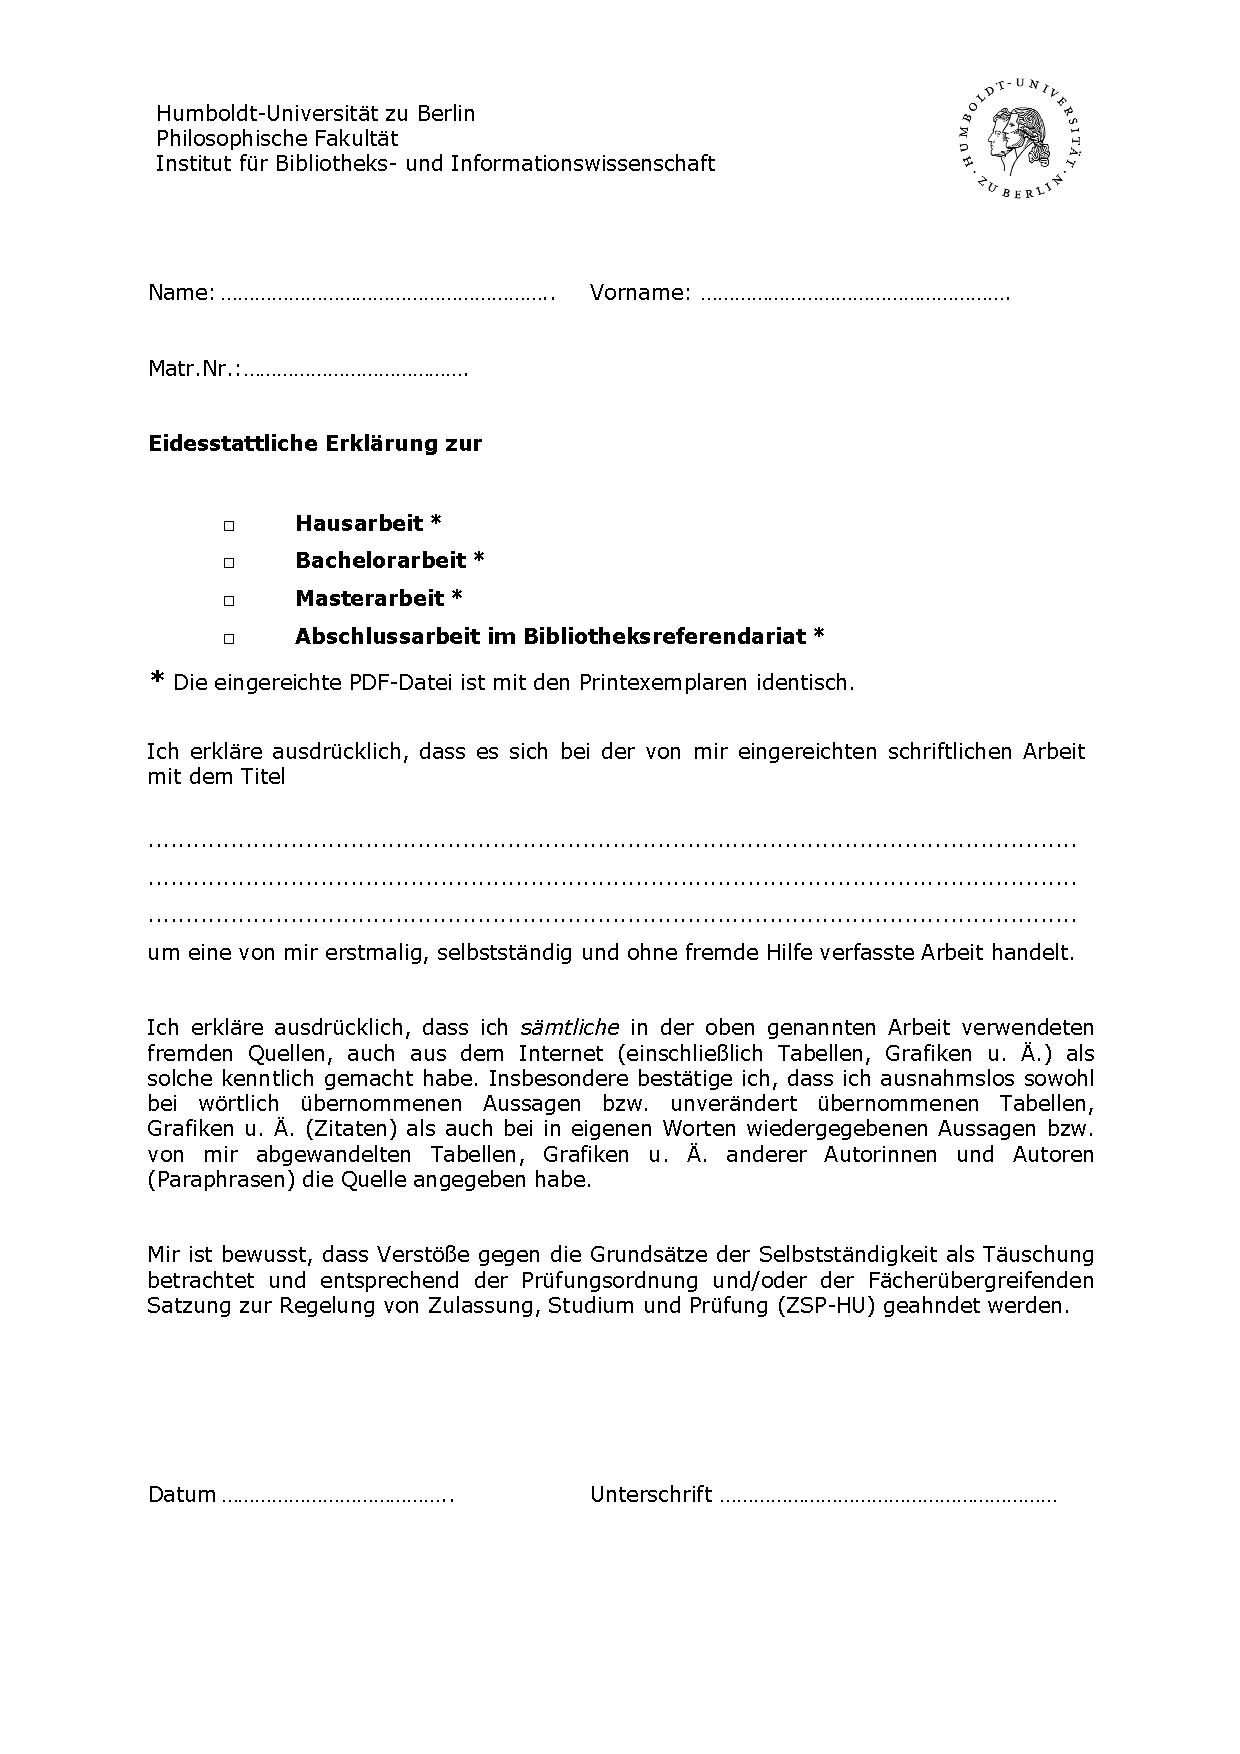
\includepdf[pages=-]{matter/backmatter/selbststaendigkeitserklaerung.pdf}
\end{document}
